%% abtex2-modelo-trabalho-academico.tex, v-1.9.6 laurocesar
%% Copyright 2012-2016 by abnTeX2 group at http://www.abntex.net.br/ 
%%
%% This work may be distributed and/or modified under the
%% conditions of the LaTeX Project Public License, either version 1.3
%% of this license or (at your option) any later version.
%% The latest version of this license is in
%%   http://www.latex-project.org/lppl.txt
%% and version 1.3 or later is part of all distributions of LaTeX
%% version 2005/12/01 or later.
%%
%% This work has the LPPL maintenance status `maintained'.
%% 
%% The Current Maintainer of this work is the abnTeX2 team, led
%% by Lauro César Araujo. Further information are available on 
%% http://www.abntex.net.br/
%%
%% This work consists of the files abntex2-modelo-trabalho-academico.tex,
%% abntex2-modelo-include-comandos and abntex2-modelo-references.bib
%%

% ------------------------------------------------------------------------
% ------------------------------------------------------------------------
% abnTeX2: Modelo de Trabalho Academico (tese de doutorado, dissertacao de
% mestrado e trabalhos monograficos em geral) em conformidade com 
% ABNT NBR 14724:2011: Informacao e documentacao - Trabalhos academicos -
% Apresentacao
% ------------------------------------------------------------------------
% ------------------------------------------------------------------------

\documentclass[
	% -- opções da classe memoir --
	12pt,				% tamanho da fonte
	openright,			% capítulos começam em pág ímpar (insere página vazia caso preciso)
	oneside,			% para impressão em recto e verso. Oposto a oneside
	a4paper,			% tamanho do papel. 
	% -- opções da classe abntex2 --
	%chapter=TITLE,		% títulos de capítulos convertidos em letras maiúsculas
	%section=TITLE,		% títulos de seções convertidos em letras maiúsculas
	%subsection=TITLE,	% títulos de subseções convertidos em letras maiúsculas
	%subsubsection=TITLE,% títulos de subsubseções convertidos em letras maiúsculas
	% -- opções do pacote babel --
	english,			% idioma adicional para hifenização
	brazil				% o último idioma é o principal do documento
	]{abntex2}

% ---
% Pacotes básicos 
% ---
%\usepackage{lmodern}			% Usa a fonte Latin Modern			
\usepackage[T1]{fontenc}		% Selecao de codigos de fonte.
\usepackage[utf8]{inputenc}		% Codificacao do documento (conversão automática dos acentos)
\DeclareUnicodeCharacter{2010}{-}
\usepackage{lastpage}			% Usado pela Ficha catalográfica
\usepackage{indentfirst}		% Indenta o primeiro parágrafo de cada seção.
\usepackage{color}				% Controle das cores
\usepackage{graphicx}			% Inclusão de gráficos
\usepackage{microtype} 			% para melhorias de justificação
% ---
\usepackage{palatino} % Use the Palatino font by default
\usepackage{amsmath}
\usepackage{nicefrac}
\usepackage{nameref}
\usepackage{placeins}
\usepackage{float}


%\usepackage[portuguese]{babel}
% ---
% Pacotes adicionais, usados apenas no âmbito do Modelo Canônico do abnteX2
% ---
% ---
\usepackage{chngcntr}
\counterwithin{figure}{section}
\usepackage[justification=centering]{caption}
% ---
% Pacotes de citações
% ---
%\usepackage[brazilian,hyperpageref]{backref}	 % Paginas com as citações na bibl
%\citeoption{abnt-substyle=COPPE}
\usepackage[alf,abnt-etal-list=0,abnt-etal-text=it,abnt-doi=doi]{abntex2cite}	% Citações padrão ABNT
% --- 
% CONFIGURAÇÕES DE PACOTES
% --- 

% ---
% Configurações do pacote backref
% Usado sem a opção hyperpageref de backref
%\renewcommand{\backrefpagesname}{Citado na(s) página(s):~}
% Texto padrão antes do número das páginas
%\renewcommand{\backref}{}
% Define os textos da citação
%\renewcommand*{\backrefalt}[4]{
%	\ifcase #1 %
%		Nenhuma citação no texto.%
%	\or
%		Citado na página #2.%
%	\else
%		Citado #1 vezes nas páginas #2.%
%	\fi}%
%% ---

% ---
% Informações de dados para CAPA e FOLHA DE ROSTO
% ---
\titulo{Solvation Free Energy Calculations of Molecules Mimicking Asphaltenes Using The SAFT-\boldmath$\gamma$ Mie Force Field}
\autor{Isabela Quintela Matos}
\local{Rio de Janeiro}
\data{2018}
\orientador{Charlles Rubber de Almeida Abreu}
\coorientador{Papa Matar Ndiaye}
\instituicao{%
  Universidade Federal do Rio de Janeiro
  \par
  Escola de Química 
  \par
  Engenharia de Processos Químicos e Bioquímicos Graduate Program}
\tipotrabalho{Dissertation (Master)}
% O preambulo deve conter o tipo do trabalho, o objetivo, 
% o nome da instituição e a área de concentração 
\preambulo{Masther's thesis presented to Engenharia de Processos Químicos e Bioquímicos graduate program, Escola de Química,
Universidade Federal do Rio de Janeiro, as
required for obtaining a Master's degree
in Chemical Engineering.}
% ---


% ---
% Configurações de aparência do PDF final

% alterando o aspecto da cor azul
\definecolor{blue}{RGB}{41,5,195}

% informações do PDF
\makeatletter
\hypersetup{
     	%pagebackref=true,
		pdftitle={\@title}, 
		pdfauthor={\@author},
    	pdfsubject={\imprimirpreambulo},
	    pdfcreator={LaTeX with abnTeX2},
		pdfkeywords={abnt}{latex}{abntex}{abntex2}{trabalho acadêmico}, 
		colorlinks=true,       		% false: boxed links; true: colored links
    	linkcolor=blue,          	% color of internal links
    	citecolor=blue,        		% color of links to bibliography
    	filecolor=magenta,      		% color of file links
		urlcolor=blue,
		bookmarksdepth=4
}
\makeatother
% --- 
\newcommand{\figref}[2][{}]{\hyperref[#2]{\figurename~\ref{#2}#1}} 

% --- Use it as \figref{label} for figures that contain only one plot, and use it as \figref[A]{label} for those figures for which you want the reference to be Figure 1A.
% Espaçamentos entre linhas e parágrafos 
% --- 

% O tamanho do parágrafo é dado por:
\setlength{\parindent}{1.3cm}

% Controle do espaçamento entre um parágrafo e outro:
\setlength{\parskip}{0.2cm}  % tente também \onelineskip

% ---
% compila o indice
% ---
\makeindex
% ---

% ----
% Início do documento
% ----
\begin{document}

% Seleciona o idioma do documento (conforme pacotes do babel)
\selectlanguage{english}
%\selectlanguage{brazil}

% Retira espaço extra obsoleto entre as frases.
\frenchspacing 

% ----------------------------------------------------------
% ELEMENTOS PRÉ-TEXTUAIS
% ----------------------------------------------------------
% \pretextual

% ---
% Capa
% ---
\imprimircapa
% ---

% ---
% Folha de rosto
% (o * indica que haverá a ficha bibliográfica)
% ---
\imprimirfolhaderosto*
% ---

% ---
% Inserir a ficha bibliografica
% ---

% Isto é um exemplo de Ficha Catalográfica, ou ``Dados internacionais de
% catalogação-na-publicação''. Você pode utilizar este modelo como referência. 
% Porém, provavelmente a biblioteca da sua universidade lhe fornecerá um PDF
% com a ficha catalográfica definitiva após a defesa do trabalho. Quando estiver
% com o documento, salve-o como PDF no diretório do seu projeto e substitua todo
% o conteúdo de implementação deste arquivo pelo comando abaixo:
%
% \begin{fichacatalografica}
%     \includepdf{fig_ficha_catalografica.pdf}
% \end{fichacatalografica}

\begin{fichacatalografica}
	\sffamily
	\vspace*{\fill}					% Posição vertical
	\begin{center}					% Minipage Centralizado
	\fbox{\begin{minipage}[c][8cm]{13.5cm}		% Largura
	\small
	\imprimirautor
	%Sobrenome, Nome do autor
	
	\hspace{0.5cm} \imprimirtitulo  / \imprimirautor. --
	\imprimirlocal, \imprimirdata-
	
	\hspace{0.5cm} \pageref{LastPage} \\
	
	\hspace{0.5cm} \imprimirorientadorRotulo~\imprimirorientador\\
	
	\hspace{0.5cm}
	\parbox[t]{\textwidth}{\imprimirtipotrabalho~--~\imprimirinstituicao,
	\imprimirdata.}\\
	
	\hspace{0.5cm}
		1. Solvation free energy.  
		2. Asphaltenes.
		3. SAFT-$\gamma$ Mie force field.
%		I. Orientador.
%		II. Universidade xxx.
%		III. Faculdade de xxx.
%		IV. Título 			
	\end{minipage}}
	\end{center}
\end{fichacatalografica}
% ---

% ---
% Inserir errata
% ---
%\begin{errata}
%Elemento opcional da \citeonline[4.2.1.2]{NBR14724:2011}. Exemplo:
%
%\vspace{\onelineskip}
%
%FERRIGNO, C. R. A. \textbf{Tratamento de neoplasias ósseas apendiculares com
%reimplantação de enxerto ósseo autólogo autoclavado associado ao plasma
%rico em plaquetas}: estudo crítico na cirurgia de preservação de membro em
%cães. 2011. 128 f. Tese (Livre-Docência) - Faculdade de Medicina Veterinária e
%Zootecnia, Universidade de São Paulo, São Paulo, 2011.
%
%\begin{table}[htb]
%\center
%\footnotesize
%\begin{tabular}{|p{1.4cm}|p{1cm}|p{3cm}|p{3cm}|}
%  \hline
%   \textbf{Folha} & \textbf{Linha}  & \textbf{Onde se lê}  & \textbf{Leia-se}  \\
%    \hline
%    1 & 10 & auto-conclavo & autoconclavo\\
%   \hline
%\end{tabular}
%\end{table}
%
%\end{errata}
% ---

% ---
% Inserir folha de aprovação
% ---

% Isto é um exemplo de Folha de aprovação, elemento obrigatório da NBR
% 14724/2011 (seção 4.2.1.3). Você pode utilizar este modelo até a aprovação
% do trabalho. Após isso, substitua todo o conteúdo deste arquivo por uma
% imagem da página assinada pela banca com o comando abaixo:
%
% \includepdf{folhadeaprovacao_final.pdf}
%
\begin{folhadeaprovacao}

  \begin{center}
    {\ABNTEXchapterfont\large\imprimirautor}

    \vspace*{\fill}\vspace*{\fill}
    \begin{center}
      \ABNTEXchapterfont\bfseries\Large\imprimirtitulo
    \end{center}
    \vspace*{\fill}
    
    \hspace{.45\textwidth}
    \begin{minipage}{.5\textwidth}
        \imprimirpreambulo
    \end{minipage}%
    \vspace*{\fill}
   \end{center}
        
   Approved dissertation. \imprimirlocal, \today:

   \assinatura{\textbf{\imprimirorientador} \\ Supervisor} 
   \assinatura{\textbf{Professor} \\ Guest 1}
   \assinatura{\textbf{Professor} \\ Guest 2}
   \assinatura{\textbf{Professor} \\ Guest 3}
   \assinatura{\textbf{Professor} \\ Guest 4}
      
   \begin{center}
    \vspace*{0.5cm}
    {\large\imprimirlocal}
    \par
    {\large\imprimirdata}
    \vspace*{1cm}
  \end{center}
  
\end{folhadeaprovacao}
% ---

%% ---
%% Dedicatória
%% ---
%\begin{dedicatoria}
%   \vspace*{\fill}
%   \centering
%   \noindent
%   \textit{ Este trabalho é dedicado às crianças adultas que,\\
%   quando pequenas, sonharam em se tornar cientistas.} \vspace*{\fill}
%\end{dedicatoria}
%% ---

% ---
% Agradecimentos
% ---
%\begin{agradecimentos}
%Os agradecimentos principais são direcionados à Gerald Weber, Miguel Frasson,
%Leslie H. Watter, Bruno Parente Lima, Flávio de Vasconcellos Corrêa, Otavio Real
%Salvador, Renato Machnievscz\footnote{Os nomes dos integrantes do primeiro
%projeto abn\TeX\ foram extraídos de
%\url{http://codigolivre.org.br/projects/abntex/}} e todos aqueles que
%contribuíram para que a produção de trabalhos acadêmicos conforme
%as normas ABNT com \LaTeX\ fosse possível.
%
%Agradecimentos especiais são direcionados ao Centro de Pesquisa em Arquitetura
%da Informação\footnote{\url{http://www.cpai.unb.br/}} da Universidade de
%Brasília (CPAI), ao grupo de usuários
%\emph{latex-br}\footnote{\url{http://groups.google.com/group/latex-br}} e aos
%novos voluntários do grupo
%\emph{\abnTeX}\footnote{\url{http://groups.google.com/group/abntex2} e
%\url{http://www.abntex.net.br/}}~que contribuíram e que ainda
%contribuirão para a evolução do \abnTeX.
%
%\end{agradecimentos}
% ---

% ---
% Epígrafe
% ---
%\begin{epigrafe}
%    \vspace*{\fill}
%	\begin{flushright}
%		\textit{``Não vos amoldeis às estruturas deste mundo, \\
%		mas transformai-vos pela renovação da mente, \\
%		a fim de distinguir qual é a vontade de Deus: \\
%		o que é bom, o que Lhe é agradável, o que é perfeito.\\
%		(Bíblia Sagrada, Romanos 12, 2)}
%	\end{flushright}
%\end{epigrafe}
% ---

% ---
% RESUMOS
% ---

% resumo em português
\setlength{\absparsep}{18pt} % ajusta o espaçamento dos parágrafos do resumo
%\begin{resumo}
% Segundo a \citeonline[3.1-3.2]{NBR6028:2003}, o resumo deve ressaltar o
% objetivo, o método, os resultados e as conclusões do documento. A ordem e a extensão
% destes itens dependem do tipo de resumo (informativo ou indicativo) e do
% tratamento que cada item recebe no documento original. O resumo deve ser
% precedido da referência do documento, com exceção do resumo inserido no
% próprio documento. (\ldots) As palavras-chave devem figurar logo abaixo do
% resumo, antecedidas da expressão Palavras-chave:, separadas entre si por
% ponto e finalizadas também por ponto.
%
% \textbf{Palavras-chave}: latex. abntex. editoração de texto.
%\end{resumo}

% resumo em inglês
\begin{resumo}[Abstract]
 \begin{otherlanguage*}{english}
  This dissertation studied the solvation free energy differences of molecules mimicking asphaltenes in different solvents with the SAFT-$\gamma$ Mie force field. Solvation free energy differences were obtained by carrying out molecular dynamics simulations at the expanded ensemble. The output from these simulations was then used to estimate the differences with the MBAR method. The results with solvents other than water had low absolute deviations in relation to the experimental data. Meanwhile, the hydration free energy calculations required a binary interaction parameter estimated with output data from molecular dynamics in order to obtain accurate free energy differences. These results indicated some problems on the SAFT-$\gamma$ Mie model for water, but, generally, proved that a coarse grained model can represent the free energy differences of the studied sets of solute-solvent.

   \vspace{\onelineskip}
 
   \noindent 
   \textbf{Keywords}: solvation free energy. asphaltenes. SAFT-$\gamma$ Mie force field.
 \end{otherlanguage*}
\end{resumo}

% ---
% inserir lista de ilustrações
% ---
\pdfbookmark[0]{\listfigurename}{lof}
\listoffigures*
\cleardoublepage
% ---

% ---
% inserir lista de tabelas
% ---
\pdfbookmark[0]{\listtablename}{lot}
\listoftables*
\cleardoublepage
% ---

% ---
% inserir lista de símbolos
%% ---
%\begin{simbolos}
%  \item[$ \Gamma $] Letra grega Gama
%  \item[$ \Lambda $] Lambda
%  \item[$ \zeta $] Letra grega minúscula zeta
%  \item[$ \in $] Pertence
%\end{simbolos}
%% ---

% ---
% inserir o sumario
% ---
\pdfbookmark[0]{\contentsname}{toc}
\tableofcontents*
\cleardoublepage
% ---



% ----------------------------------------------------------
% ELEMENTOS TEXTUAIS
% ----------------------------------------------------------
\textual

% ----------------------------------------------------------
% Introdução (exemplo de capítulo sem numeração, mas presente no Sumário)
% ----------------------------------------------------------
\chapter{Introduction} % Main chapter title
\label{Chapter1} % 
\pagestyle{simple}
\onehalfspacing
Solvation free energy calculations with molecular dynamics (MD) have a variety of applications ranging from drug design in the pharmaceutical industry to the development of separation technologies in the chemical industry. {Solvation free energy is, more specifically, the difference in free energy related to the process of transferring a solute from an ideal gas phase into a liquid solution \cite{shirts2013}}. Through the study of the solvation phenomenon, it is possible to obtain information about the behavior of the solvent in different thermodynamic conditions and the influence of the solute's molecular geometry. It is also possible to calculate other important properties with the solvation free energy, namely the activity coefficient at infinite dilution, Henry constant, and partition coefficients.{ Additionally, solvation free energy calculations can be part of the methodology of calculating solubility from molecular dynamics}. 

The solvation free energy calculations described above are intrinsically complex due to the many competing forces interfering in the behavior of the solute-solvent interaction. In addition, free energy simulations are susceptible to sampling problems in low energy regions, and simulation results need to be correctly post-processed in order to yield free energy differences with small uncertainties. {Another influencing factor in the output of these calculations is the choice of force field used to model the solvent and solute molecules. Force field is the name given to the group of parameters and equations used to represent the potential energy function of a system in molecular simulations. They have different levels of description, such as quantum mechanics, atomistic, and coarse-grained. The quantum mechanics approach describes the motion of electrons and requires for the solution of the Schr\"{o}dinger equation during the simulation. In the atomistic description, only the atomic motions are represented,  and this is done by solving Newton's equations of motion. Finally, in the coarse-grained description, atoms are grouped into pseudo-atoms or beads, and the equations of motion are solved for them. 
	
These coarse-grained models are generally able to reproduce experimental free energy differences since the effects of reducing degrees of freedom in the entropy are counterbalanced by the reduction of enthalpic terms \cite{kmiecik2016}. This fact makes these models a viable option to decrease the computational time of solvation free energy calculations. Additionally, deficiencies in the description of small molecules by coarse-grained models can be revealed by free energy calculations \cite{mobley2007,shirts2013}. Hence, we, in this study, assess the performance and shortcomings of the SAFT-$\gamma$ Mie coarse-grained force field  \cite{avendano2011} with free energy calculations of a variety of solute-solvent pairs. We choose this coarse-grained force field because it uses, unlike the majority of the force fields, the Mie potential \cite{MIE} and because its method of obtaining parameters is more straightforward than those of other models. It was initially parameterized with pure component equilibrium and interfacial tension data \cite{avendano2011}, and this strategy has provided satisfactory results. Examples include the prediction of phase equilibrium of aromatic compounds \cite{muller2017}, alkanes, light gases \cite{herdes2015}, and water \cite{lobanova2015}, thermodynamic properties of carbon dioxide and methane \cite{cassiano1}, multiphase equilibrium of mixtures of water, carbon dioxide, and n-alkanes \cite{lobanova2016}, and water/oil interfacial tension \cite{herdes2017}.} 


We selected the solvents and solutes in our free energy calculations with the intention of testing the force field with standard sets used as a benchmark in solvation free energy calculations and with polycyclic aromatic substances used as models to asphaltenes. Asphaltenes are complicated to characterize by determining their composition on a molecular basis, but the literature broadly accepts that they can be described as a fraction of crude oil soluble in toluene and insoluble in n-alkanes (pentane, hexane, heptane) \cite{SJOBLOM2003399}. They have motivated many studies with interest in developing models for their structure and behavior due to all the problems they can cause during their transportation and refining such as precipitation during the oil processing \cite{SJOBLOM20151}. This precipitation issue is a recurrent problem due to the growing market of the production of crude oil in deep waters, whose conditions are favorable to precipitation \cite{AIC:AIC10243}. As an example, asphaltene precipitation due to pressure drop can clog oil production equipment and cause a growth in the cost of production \cite{doi:10.1021/ef010047l}. All these factors make the understanding of the behavior of asphaltenes in different chemical and physical environments relevant to the oil industry. 

As said in the previous paragraph, asphaltene characterization still faces some issues. Hence, we choose to use polycyclic aromatic hydrocarbons (PAHs), which have well-defined characteristics, to initially test the efficiency of the SAFT-$\gamma$ Mie force field in describing the solvation phenomenon. PAHs are a group of organic compounds that have fused rings, carbon and hydrogen in their structure \cite{RAVINDRA20082895}. The ones utilized in this work were phenanthrene, anthracene, and pyrene since they share similarities with asphaltenes regarding their solubility. In this context,  we selected compounds that are used to characterize asphaltenes (toluene, hexane) as solvents in our free energy calculations. We also tested the anti-solvent/solvent effect of carbon dioxide due to its influence in asphaltene precipitation during the oil processing \cite{SOROUSH2014405}. With these calculations of solvation free energies with the SAFT-$\gamma$ Mie model, we intend to improve this force field and provide satisfactory solvation free energy estimates of PAHs with a coarse-grained model. The success of the description of small asphaltene-like compounds by this force field can then open up the possibility of obtaining satisfactory results for more complex asphaltene models with a force field with a low computational cost.


% Chapter Template

\chapter{Literature Review} % Main chapter title

\label{Chapter2} % Change X to a consecutive number; for referencing this chapter elsewhere, use \ref{ChapterX}

%----------------------------------------------------------------------------------------
%	SECTION 1
%----------------------------------------------------------------------------------------

\section{Coarse Grained Force Fields}

Molecular simulations can be carried out at different levels of descriptions. The detailed atomistic level or \textit{ab initio}level is described by the laws of quantum mechanics. The system consists of a set of subatomic particulars in which Schrodinger's equation is solved for all of them. The next level is the atomistic description. It considers that the system is made up of atoms following the laws of statistical mechanics.  Force fields at this level are based on pair potentials with Coulombic charged sites, which account for the molecular interactions. The contributions due to to intramolecular interactions like bond-stretching, angle-bending and torsion are also usually accounted by these kind of force fields. When the scale of the simulations needs to be increased and the atomistic simulations become too computationally expensive, the coarse-grained (CG) description is more suited. It considers that the system is made up of pseudo atoms or beads that contain multiple atoms. 

There is a obvious loss of information in grouping atoms, hence it is necessary to assure that the process of eliminating unnecessary or unimportant information ('coarse graining') doesn't affect the system's physical behavior. The coarse grained force fields are developed by mapping the atomistic model to define the pseudo atoms with the intetion of assuring that the model has accuracy, transferability, robustness, and computational efficiency. This mapping is normally done by grouping similar funcional groups. The level of coarse-graining also needs to be defined, up to 6 heavy atoms (non-hydrogen atoms) per bead in order to not loose much detail and maintain isotropic representations of the beads \cite{shinoda2007,martini2007,hadley2012}. The CG force field can be parametrized following two different approaches: bottoms up and top down. The bottoms up approach uses information of a more detailed scale such as the \textit{ab initio} description or the atomistic description to obtain the information necessary to the parametrization. This method depends highly of the quality of the detailed model to succeed. Meanwhile, the top down methodology obtains the parameters from one larger scales. This information at larger scales could be experimentally observed data like thermodynamic properties or native-structure based properties. 

One of the first applications of coarse grained models is the study of protein folding \cite{levitt1975,levitt1976}. These earlier protein CG models were based on the structure of the molecule and they contributed for the knowledge of the physicochemical forces associated with protein folding and protein interactions \cite{koga2001}.  More recent models focused on retaining the protein's chemical specificity. The Bereau and Deresmo model \cite{bereau2009} has a up to four-bead representation and was used in studies of protein folding and aggregation. However, this model still needs tuning to improve stability of proteins \cite{bereau2010}. The OPEP (Optimized Potential for Efficient Protein Structure Prediction) model \cite{opep2014,opep2015} has up to six-bead representation. It was used to investigate a variety of phenomena, ranging from protein folding to \textit{ab initio} peptide structure prediction \cite{opep2011,opep2009,opep20092}. Other CG protein models used in the literature are the Scorpion (solvated coarse-grained protein interaction)  \cite{scorpion2013}, the UNRES (united residue) \cite{unres2014} and the MARTINI model \cite{martini2013}. The later one is the most popular model for the CG modeling of membrane proteins \cite{martini20132}. The MARTINI model is also extensively used as CG model for water. This model represents four water molecules as one bead using a shifted Lennard Jones potential for the non bonded interactions. Though its extensive use, the MARTINI water model doesn't properly represent properties as interfacial tension and compressibility \cite{shinoda2010} and can freeze at room temperature \cite{winger2009,martini2007}, what makes necessary the use of anti-freeze agents during the simulations. This behavior can be explained by the high level of coarse graining (4:1), the lack of explicit charges and the use of the 12-6 potential. With the idea of improving the MARTINI model, \citeonline{chiu2010} used the Morse Potential, which is softer than the LJ potential. Meanwhile, \citeonline{shinoda2007} used different forms of the Mie potential. They concluded that a 12-4 Mie Potential was ideal for the all water cross interactions and  a 9-6 Mie Potential was suited for all the solute-solute interactions. 

Outside of the Martini framework, \citeonline{shinoda2010} studied different levels of coarse-graining for water ranging for one to 4 molecules per bead using different Mie and Morse potentials. Other works also assessed the use of Soft-core potentials to study aqueous solutions of surfactants \cite{shinoda2007}, ionic liquids \cite{bhargava2009}, lipids \cite{shinoda20102} and membranes \cite{pantano2009}. Other CG force field for water based on the Mie Potential is the SAFT-$\gamma$ Mie \cite{lobanova2015}. In this model, the water molecule can be represented by two different one isotropic bead interacting via a 8-6 Mie Potential models. The CGW1-vle model was parametrized using saturated-liquid density and vapor pressure data, and should be used for simulations of aqueous systems' fluid-phase equilibria at high temperatures and pressures. This model still suffers from premature freezing with a triple point at 343 K. The other model, CGW1-ift, was parametrized using saturated-liquid density and vapor-liquid interfacial tension, hence it is best suited for interfacial properties calculations. Both models have temperature-dependent size and energy parameters and performed well for these properties over the entire temperature range of the liquid. The SAFT-$\gamma$ Mie force field have also been applied to other compounds with satisfactory results. \citeonline{muller2017} parametrized the force field for aromatic compounds and tested it with simulations of fluid phase equilibrium. \citeonline{herdes2015} carried out simulations of alkanes and light gases with this force fields. Binary and ternary mixtures of water, carbon-dioxide and water \cite{lobanova2016}, thermodynamic and transport properties of carbon dioxide and methane \cite{cassiano1,cassiano2} and water/oil interfacial tension \cite{herdes2017} were also studied with this force field.   

\section{Solvation Free Energies Based on Molecular Dynamics}

Free energies can be expressed as averages over ensembles of atomic configurations generated using Monte Carlo or molecular dynamics techniques. In the canonical ensemble, the free energy is given by:  

\begin{equation}
\label{eq:fcano}
\begin{aligned}
F(N,V,T) = -\kappa_{b}TQ(N,V,T)
\end{aligned}
\end{equation}
where $Q(N,V,T))$ is the partition function of the canonical ensemble. Meanwhile, the average over the isothermal-isobaric ensemble gives the Gibbs free energy:

\begin{equation}
\label{eq:fisobari}
\begin{aligned}
G(N,P,T) = -\kappa_{b}T\frac{1}{V_{0}} \int_{0}^{\infty} dV \exp(-\kappa_{b}TPV)Q(N,V,T)
\end{aligned}
\end{equation}

Since it is only possible to obtain free energy differences, Solvation free energy calculations based on molecular dynamics estimate the difference between the Gibbs free energies of end states, more specifically the difference between the solute alone in the gas phase and the solute interacting with the solvent. In order to these energy differences be accurate, the sates' phase integral must have sufficient overlap  \cite{klimovich}. This can be achieved by calculating the free energy difference between a series of intermediates states. The result of these differences are independent of the path chosen since the free energy is a state function. That's why the states used typically don't have a physical sense, they are alchemical states which are only linking the physical states of interest.

The solvation free energy calculations follow a thermodynamic cycle to gradually insert the solute molecule into the solvent as illustrated in the \figref{thermcy}. According to this cycle, the free energy of solvation can be expressed as:

\begin{equation}
\label{eq:freesolv}
\begin{aligned}
\Delta G_{solv} = \Delta G_{1 \rightarrow 4} = \Delta G_{1 \rightarrow 2} + \Delta G_{2 \rightarrow 3} + \Delta G_{3 \rightarrow 4}  
\end{aligned}
\end{equation}


\begin{figure}[th]
\centering
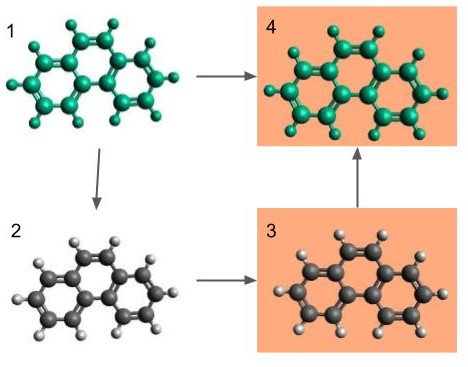
\includegraphics[scale=0.6]{Figures/cicclotermo.jpg}
\caption{Thermodynamic cycle for solvation free energy calculations with molecular dynamics (Adapted from \citeonline{klimovich})}
\label{thermcy}
\end{figure}

The solvation free energy between sates 1 and 2 in the cycle is the one associated with turning off the molecule's non bonded interactions in the gas phase. The following transformation, $\Delta G_{2 \rightarrow 3}$, is the free energy of moving the non-interacting molecule in the gas phase to the solvent and is equal to zero since the transformation of a non interacting molecule doesn't depend on the environment. Lastly, $\Delta G_{3 \rightarrow 4}$ is the free energy required to the  the non-interaction molecule in the aqueous phase regain its non-bonded interactions.  The solvation free energy calculation can be classified according to the types of the non bonded interactions that are turned of in the $1 \rightarrow 2$ and $ 3 \rightarrow 4$ parts of the cycle. If both the non-bonded interactions with the environment and the internal interactions are turned of, this is the annihilation free energy. Meanwhile, if only the non-bonded interactions with the environment are turned off,this is the decoupling free energy. In this later case, $\Delta G_{1 \rightarrow 2} = 0$ and the $\Delta G_{solv} = \Delta G_{3 \rightarrow 4} $. The methods used to carry out theses transformations scale the solute charges to zero and then turn of the interactions corresponding to the Lennard Jones potential. In order to carry out the later process, a modified potential with a coupling parameter $\lambda$ is used. Each $\lambda$ represent an alchemical state and, when $\lambda=0$, there is no interaction with the solvent and, when $\lambda=1$, the interactions are fully activated. The coupling of the $\lambda$ parameter could be linear, but it could generate numerical problems related to the exponential part of the Potential. That's why the non-linear soft-core scheme \cite{beutler1994} is usually used, the so called soft core Lennard-Jones potential is given by:

\begin{equation}
\label{eq:softcore}
\begin{aligned}
U_{LJ}^{sc}(r) {}=& 4\lambda\epsilon \left\lbrace\frac{1}{\left[\alpha(1-\lambda)^{2}+ (r/\sigma)^{6}\right]^{2}} - \frac{1}{\alpha(1-\lambda)^2+(r/\sigma)^{6}}\right\rbrace
\end{aligned}
\end{equation}
where $\alpha$ is a constant in which the value of 0.5 is normally assumed to it. The $\Delta G_{3 \rightarrow 4}$ can be then obtained by doing independent simulations in different values of $\lambda$ or by doing expanded ensemble simulations \cite{lyubartsev} which samples all state in a single simulation. This method allows a faster sampling across the alchemical states considering that the kinetic barriers are not substantial. 

\section{Post simulation methods}

The data obtained with molecular dynamics simulations method explained in the section above contain the potential energies correspondent to each $\lambda$. These potential energies obtained then needs to be post processed and analyzed in order to calculate the solvation free energies. Some of the widely used method for these calculations are going to be briefly describe below. 

\subsection{Thermodynamic integration}

The thermodynamic integration method \cite{kirkwood1935} uses equilibrium averages to evaluate the derivative of the potential energy with respect to the coupling parameter. Then, the free energies are obtained as the integration of the derivatives of the initial and final state:

\begin{equation}
\label{eq:ti}
\begin{aligned}
\Delta G_{solv} = \int_{0}^{1} \frac{\partial U}{\partial \lambda} d\lambda
\end{aligned}
\end{equation}

The integration in Eq. \eqref{eq:ti} is obtained by interpolating the output data form the simulations in different ways. Some examples of methods for the interpolations are the trapezoidal rule or natural cubic spline \cite{bareva}. There are also other more complex schemes that are usually system specific as the works of \citeonline{garrido2010} and \citeonline{shyu2009} and that use fitting functions to interpolate the data. 

\subsection{Free energy of Pertubation (FEP)}

The free energy of perturbation method \cite{zwanzig1954} is the oldest and the of the most general purpose strategy to calculate free energy differences. In this method, the difference between two thermodynamic states A and B is given by:

\begin{equation}
\label{eq:fep}
\begin{aligned}
\Delta F = -\kappa_{b}ln \langle{e^{-\beta (U_{B}-U_{A})}}\rangle_{A}
\end{aligned}
\end{equation}

According to the equation above, the free energy difference is calculated by doing an average over the potential energies of state A and B obtained during the simulation of state A. This method only provides precise free energies when there  is a great overlap between the state that is, the state B represents a small perturbation in state A. 

\subsection{Bennet Acceptance Ratio (BAR)}


 En realidad, cuando se simulan
dos estados existe un método que asegura convergencia en el cálculo de deltaF sin exigir un
solapamiento considerable de las distribuciones configuracionales. En particular, nos estamos
refiriendo al método Bennett Acceptance Ratio [148], que describimos en la próxima sección.

%Recent work \cite{mobley2014,mobley2017} made available a big database of hydration free energy of small molecules using the GAFF force field. A comparision of polar and nonpolar contributions to these hydratation free energy inidcated the significance of each the terms  \cite{izairi2017}. Garrido \textit{et al.} \citep{garrido,garrido2011} calculated the free energy of solvation of large alkanes in 1-octanol and water with three different force fields (TraPPE, Gromos, OPLS-AA/TraPPE) and the solvation free energy of propane and benzene in non aqueous solvents like n-hexadecane, n-hexane, ethyl benzene, acetone  with the force fields TraPPE-UA and TraPPE-AA. Roy \textit{et al.} \citep{roy2017} addressed the choice of the Lennard Jones parameters for predicting solvation free energy in 1-octanol. Gon\c{c}alves and Stassen \citep{goncalves} calculated the free energy of solvation in the solvents tetrachloride, chloroform and benzene with GROMOS force field. Using the GAFF and the polarazible AMOEBA force fields, Mohamed \textit{et al.} \citep{mohamed2016} evaluated the solvation free energy of small molecules in toluene, chloroform and acetonitrile and obtained a mean unsigned error of 1.22 $kcal/mol$ for the AMOEBA and 0.66 $kcal/mol$ for the GAFF. 



benchmark
Specifically, in some
situations, free energy calculations appear to be capable
of achieving RMS errors in the 1-2 kcal/mol range with
current force fields, even in prospective applications.

The most immediate application of these techniques is to guide synthesis for lead optimization, but applications to scaffold
hopping and in other areas also appear possible.

At the same time, it is clear that not all situations are
so favorable, so it is worth asking what level of accuracy
is actually needed

The present review focuses on a class of methods in
which free energy differences are computed with simulations that sample Boltzmann distributions of molecular configurations. These samples are usually generated by molecular dynamics (MD) simulations [92], with
the system effectively coupled to a heat bath at constant temperature, but Monte Carlo methods may also
be used [32, 120, 121]. 

In either case, the energy of a
given configuration is provided by a potential function,
or force field, which estimates the potential energy of
a system of solute and solvent molecules as a function
of the coordinates of all of its atoms.

In
all cases, however, the calculations yield the free energy
difference between two states of a molecular system, and
they do so by computing the reversible work for changing
the initial state to the final one. 
 

\chapter{Computational Methods} % Main chapter title

\label{Chapter3} % Change X to a consecutive number; for referencing this chapter elsewhere, use \ref{ChapterX}
%\doublespacing

\section{Molecular Dynamics}

\subsection{Background and Formulation}
Molecular Dynamics (MD) uses molecular configurations (Cartesian coordinates and momentum) to extract structural, thermodynamic, and dynamic information of a system. This information is extracted from the time evolution of the system, which is obtained  through the numerical integration of the Newton's equations of motion \cite{tuckerman}:

\begin{equation}
\frac{d \vec{p}_{i}}{dt} = - \frac{\partial U (\vec{r}_{N})}{\partial \vec{r}_{i}},
\end{equation}
where $p_{i}$ is the momentum and $r_{N}$ are the coordinates of all the atoms $(x_{1},y_{1},z_{1},..., x_{N},\\ y_{N},z_{N})$. Alternatively, we can write the equation relative to the velocity ($v_{i}$):
\begin{equation}
m_{i} \frac{\vec{v}_{i}}{dt} = - \frac{\partial U (\vec{r}_{N})}{\partial \vec{r}_{i}}.
\end{equation}

In order to develop equations for any coordinate system, for instance $q^{N}=(r_{1},\theta _{1},\phi _{1})$, the Hamiltonian formulation, a more general formulation of classical mechanics,  is used to develop the equations of motion:
\begin{equation}
\mathcal{H} (q^{N},p^{N}) = K(p^{N}) + U(q^{N}) .
\end{equation}

In the equation above, $K$ is the kinetic energy and $U$ is the potential energy. The equations of motion are then rewritten using the Hamiltonian:

\begin{equation}
\frac{d \vec{p}_{i}}{dt} = - \frac{\partial \mathcal{H}}{\partial \vec{q}_{i}},
\end{equation}

\begin{equation}
\frac{d \vec{q}_{i}}{dt} =  \frac{\partial \mathcal{H}}{\partial \vec{q}_{i}}.
\end{equation}

In the dynamics described by the equations above, the Hamiltonian is preserved. The coordinate and momentum axes for each atom in a 6N dimensional space is defined as the phase space. The trajectory through the phase space is then the time evolution of a system in a molecular dynamics simulation. This evolution of the simulation may be used to calculate the thermodynamic properties if the system is ergodic, that is, a trajectory in this system will explore with the same probability all regions of the phase space of microstates (points in phase space) with the same energy \cite{shell2015}. 

\subsection{Statistical Ensembles}

In order to calculate thermodynamic properties, we need to define the control variables of a system. For an isolated system at equilibrium, the control variables are the number of particles (N), volume (V), and total energy (E). The set of configurations under the control variables is then called statistical ensemble. In the example cited above, it is specifically named the microcanonical ensemble. Following the ergodic hypothesis, the system at these conditions will spend the same amount of time in each of the microstates  with the fixed Hamiltonian.  The number of accessible microstates is defined by the partition function or the density of states, and  is given by the following equation  for the microcanonical ensemble: 

\begin{equation}
\begin{aligned}
\Omega (N,V,E) = \frac{\epsilon_{0}}{h^{3N}N!} \int dp^{N} dr^{N} \delta [\mathcal{H}(p^{N},r^{N}) -E].
\end{aligned}
\end{equation}

Here, $\epsilon _{0}$ is the energy unit, $h$ is the Planck constant, and $\delta$ is the Dirac delta function. As mentioned above, the system will spend the same amount of time at each of the microstates, i. e. each of these microstates have equal probabilities ($\varrho$) of being visited. Such probability is:

\begin{equation}
\begin{aligned}
\varrho (p^{N},r^{N}) = \frac{[\mathcal{H}(p^{N},r^{N}) -E]}{ \Omega (N,V,E)} .
\end{aligned}
\end{equation}

The macroscopic properties from molecular dynamics are then obtained from the relation of the microcanonical partition function to the entropy ($S$). Known as the Boltzmann equation. It is:

\begin{equation}
\begin{aligned}
S = \kappa_{b} ln [\Omega (N,V,E)], 
\end{aligned}
\end{equation}
where $\kappa_{b}$ is the Boltzmann constant. With these equations, we can derive other relations to macroscopic properties with the fundamental thermodynamic equations:

\begin{equation}
\begin{aligned}
dS = \frac{1}{T} dE + \frac{P}{T} dV + \frac{\mu}{T} dN,
\end{aligned}
\end{equation}

\begin{equation}
\begin{aligned}
dE = T dS + P dV + \mu dN .
\end{aligned}
\end{equation}

As said above, the microcanonical ensemble  has  N, V, and E as its control variables. Other ensembles can also be defined according to the macroscopic properties held constant.  In the canonical ensemble,  N, V, and the temperature (T) are held constant and  N, pressure (P), and T are held constant in the isothermal-isobaric ensemble. Other ensembles are the isoenthalpic-isobaric (constant number of particles, pressure, and enthalpy) and the grand canonical (constant chemical potential, volume, and temperature) ones. A variety of physical properties is measured at the conditions of the isothermal-isobaric ensemble such as enthalpies, entropies, redox potential, equilibrium constants, and free energies, what makes this ensemble one of the most important \cite{tuckerman}. This is also the ensemble in which solvation free energy simulations are carried out at this work, hence we are going to briefly talk about it. This ensemble is obtained from a Legendre transformation on the canonical ensemble. The Helmholtz free energy $A(N,V,T)$ becomes the Gibbs free energy $G(N,P,T)$ by transforming the volume into the external pressure:
\begin{equation}
G(N,P,T) = A(N,V,T) + PV,
\end{equation}
where $V = V(P)$. The Gibbs free energy is related to its partition function $\Delta (N,P,T)$ by:

\begin{equation}
\label{eq:fisobari}
\begin{aligned}
G(N,P,T) = -\kappa_{b}T ln \Delta (N,P,T),
\end{aligned}
\end{equation}
where $\Delta (N,P,T)$ is given by: 

\begin{equation}
\begin{aligned}
\Delta (N,P,T) = \frac{1}{V_{0}} \int_{0}^{\infty} dV \int d p^{N} d r^{N} \exp \left[ -\beta \left( \mathcal{H} (r^{N},p{N}) + PV(r^{N}) \right) \right] .
\end{aligned}
\end{equation}

In the equation above, $Q (N,V,T)$ is the partition function of the canonical ensemble:

\begin{equation}
\begin{aligned}
Q(N,V,T) = \int d^{N}p d^{N}r \exp \left[ -\beta \mathcal{H} (r^{N},p{N}) .
\right]
\end{aligned}
\end{equation}

From these relations and a differential change in G, we can obtain the chemical potential ($\mu$), volume and entropy relations for isothermal-isobaric ensemble:

\begin{equation}
\mu = \left (\frac{\partial G}{\partial N} \right)_{P,T} = - \kappa_{b} T \left(\frac{\partial ln \Delta (N,P,T)}{\partial N} \right)_{N,T},
\end{equation}  
\begin{equation}
\langle V \rangle= \left (\frac{\partial G}{\partial P} \right)_{N,T}= \kappa_{b} T \left (\frac{\partial ln \Delta (N,P,T)}{\partial N} \right)_{N,P},
\end{equation}
\begin{equation}
S = \left (\frac{\partial G}{\partial T} \right)_{N,P}= \kappa_{b}  \left[ln Q(N,V,T)+ T \left (\frac{\partial ln Q (N,V,T)}{\partial T} \right)_{V,N}\right] .
\end{equation}

\subsection{Thermostats and Barostats}

The isothermal-isobaric and canonical ensembles have external conditions being applied to it (temperature and pressure). For temperature control, the method employed mimics the effect of a thermal reservoir through the use of a thermostat. The thermostats need to be capable of capturing the correct energy fluctuations in the system since the kinetic energy will fluctuate when using a heat bath to control the temperature in a canonical ensemble of a finite system \cite{frenkel}.  

Among the available thermostat are the Berendsen \cite{doi:10.1063/1.448118}, the Andersen \cite{1980JChPh722384A}, and the Nos\'{e} \cite{1984JChPh81511N} thermostats, but, here, we are going to discuss the most widely used thermostat: the Nosé-Hoover \cite{PhysRevA.31.1695}. This thermostat is based on the formulation of Nosé \cite{1984JChPh81511N}, who used a Lagrangian that contains additional and artificial coordinates and velocities \cite{frenkel}. In this method, the Hamiltonian in a canonical ensemble is constructed as:

\begin{equation}
\mathcal{H}_{Nos\acute{e}} =  K(p^{N}) + U(q^{N})  + \frac{\xi ^{2} \mathcal{Q}}{2} + 3N\kappa_{b}T ln s ,
\end{equation}
where $\xi$ is a friction coefficient related to the conjugate momentum of the thermal reservoir to which the system is coupled, $s$ is the position of the thermal reservoir, and $\mathcal{Q}$ is the effective mass associated with s. The velocity update is then done with the friction term added to the equations of motion \cite{shell2015}:

\begin{equation}
\frac{dr_{i}}{dt} = \frac{p_i}{m_i},
\end{equation}

\begin{equation}
\frac{dp_{i}}{dt} = -  \frac{\partial U (r^{N})}{\partial r_{i}} - \xi p_{i},
\end{equation}

\begin{equation}
\frac{\xi}{dt} = \frac{\sum p_{i}^{2}/m_{i} - 3N\kappa_{b}T}{\mathcal{Q}} ,
\end{equation}

\begin{equation}
\frac{1}{s}\frac{ds}{dt} =\frac{d \ln s}{dt} = \xi.
\end{equation}

This approach proposed by the Nos\'{e}-Hoover thermostat only generates a correct canonical distribution for molecular systems in which there are no external forces ($F_{i}$) and the center of mass is fixed or if there is only one conserved quantity \cite{frenkel}. To diminish these restrictions of the Nosé-Hoover thermostat, the Nosé-Hoover chains of thermostats method was developed by \citeonline{doi:10.1063/1.463940}. This is the one chosen to control the temperature in our simulations. It proposes the use of another thermal reservoir or a whole chain of thermal reservoirs in order to enhance temperature equilibration \cite{shell2015}. Here, we are going to present its equations of motion since this was the method used in this dissertation. The equations of motion of a system of N particles coupled with M Nos\'{e}-Hoover chains is given by

\begin{equation}
\frac{dr_{i}}{dt} = \frac{p_i}{m_i},
\end{equation}

\begin{equation}
\frac{dp_{i}}{dt} = F_i  - \frac{p_{\xi _{1}}}{\mathcal{Q} _1} p_{i},
\end{equation}

\begin{equation}
\frac{\xi _{k}}{dt} = \frac{p_{\xi _k}}{\mathcal{Q} _{k}} \quad k = 1,...,M ,
\end{equation}

\begin{equation}
\frac{p_{\xi _1}}{dt} = {\sum p_{i}^{2}/m_{i} - 3N\kappa_{b}T} -  \frac{p_{\xi _{2}}}{\mathcal{Q} _2}p_{\xi _{1}},
\end{equation}

\begin{equation}
\frac{p_{\xi _k}}{dt} = \frac{p_{\xi _{k -1}}^{2}}{\mathcal{Q} _{k-1}} - \kappa_{b}T - \frac{p_{\xi _{k+1}}}{\mathcal{Q} _{k+1}}p_{\xi _{k}},
\end{equation}

\begin{equation}
\frac{p_{\xi _M}}{dt} = \frac{ p_{\xi _{M-1}}^{2}}{\mathcal{Q} _{M-1}} - \kappa_{b}T .
\end{equation}

The conserved energy for the Nos\'{e} Hoover chains is then equal to

\begin{equation}
\mathcal{H}_{Nos\acute{e} \, Chains} =  K(p^{N}) + U(q^{N})  + \sum_{k=1}^{M }\frac{p^{2}_{\xi _{k}}}{2\mathcal{Q} _{k}} + 3N\kappa_{b}T \xi _{1} + \sum_{k=2}^{M} \kappa_{b}T \xi _{k}.
\end{equation}

The pressure is controlled with a barostat. It maintains the pressure constant during the simulation by adjusting the simulation volume. Among the available  barostats methodologies are the Berendsen \cite{doi:10.1063/1.448118}, in which the pressure is coupled to a pressure bath, and the volume is periodically rescaled, and the Anderson barostat \cite{1980JChPh722384A}, which serves as a basis for other barostating methods such as the ones developed by Hoover \cite{PhysRevA.31.1695}, Martina-Tobias-Klein \cite{doi:10.1063/1.467468} and Parrinello-Rahman \cite{doi:10.1063/1.328693}. The Andersen's idea was to couple the system to a fictional pressure bath and incorporate the volume into the phase space as an additional degree of freedom \cite{tuckerman}. Here, we are going to present the approach developed by \citeonline{doi:10.1063/1.467468} since this was the one used to control the pressure in our simulations. The equations of motion for a chain of barostats of length M are given by  

\begin{equation}
\frac{dr_{i}}{dt} = \frac{p_i}{m_i} + \frac{p_{\epsilon}}{\mathcal{W}} r_i,
\end{equation}

\begin{equation}
\frac{dp_{i}}{dt} = F_i  - \left(1 + \frac{d}{dN}\right) \frac{p_{\epsilon}}{\mathcal{W}} p_{i} - \frac{p_{\epsilon _{1}}}{\mathcal{Q} _1} p_{i},
\end{equation}

\begin{equation}
\frac{dV}{dt} = \frac{d V p_{\epsilon}}{\mathcal{W} }
\end{equation}

\begin{equation}
\frac{dp_{\epsilon}}{dt} = dV (    P_{int} -P_{ext}) + \frac{1}{N} \sum_{i=1}^{N} \frac{p_{i}^{2}}{m_i} - \frac{p_{\xi _{1}}}{{\mathcal{Q} _1}}p_{\epsilon},
\end{equation}

\begin{equation}
\frac{\xi _{k}}{dt} = \frac{p_{\xi _k}}{\mathcal{Q} _{k}} \quad k = 1,...,M ,
\end{equation}

\begin{equation}
\frac{p_{\xi _1}}{dt} = \sum \frac{p_{i}^{2}}{m_{i}} - \frac{p_{\epsilon}^{2}}{\mathcal{W}} -  (dN +1)\kappa_{b}T -\frac{p_{\xi _{2}}}{\mathcal{Q} _2}p_{\xi _{1}},
\end{equation}

\begin{equation}
\frac{p_{\xi _k}}{dt} = \frac{p_{\xi _{k -1}}^{2}}{\mathcal{Q} _{k-1}} - \kappa_{b}T - \frac{p_{\xi _{k+1}}}{\mathcal{Q} _{k+1}}p_{\xi _{k}} \quad k = 2,...,M-1 ,
\end{equation}

\begin{equation}
\frac{p_{\xi _M}}{dt} = \frac{ p_{\xi _{M-1}}^{2}}{\mathcal{Q} _{M-1}} - \kappa_{b}T .
\end{equation}

In the equations above, $\epsilon$ is equal to

\begin{equation}
\epsilon = \ln \left[\frac{V}{V(0)}\right],
\end{equation}
where $V$ is the volume of the system and $V(0)$ is the volume at $t=0$. The mass parameter ($\mathcal{W}$) associated to $\epsilon$, the momentum ($p_{\epsilon}$) conjugate to $\epsilon$, the external pressure ($P_{ext}$), and the internal pressure ($P_{int}$) are also featured in the equations of motion. $P_{ext}$ is imposed as we do with the temperature in the thermostat and $P_{int}$ is calculated during the simulation with the following equation \cite{tuckerman}:

\begin{equation}
P_{int} = \frac{1}{dV} \left[\sum_{i=1}^{N} \left(\frac{p_{i}^2}{m_i} + r_{i}\cdot F_i \right) - dV \frac{\partial U}{\partial V}\right].
\end{equation}


Finally, the conserved energy for the chain of barostats proposed by \citeonline{doi:10.1063/1.467468} is equal to

\begin{equation}
\mathcal{H}_{N,P_{ext},T} =  K(p^{N}) + U(q^{N})  + \frac{p_{\epsilon}^2}{\mathcal{W}}+\sum_{k=1}^{M }\frac{p^{2}_{\xi _{k}}}{\mathcal{Q} _{k}} + (dN+1)\kappa_{b}T \xi _{1}  + \kappa_{b}T\sum_{k=1}^{M}  \xi _{k} + P_{ext}V.
\end{equation}

All the equations of motion above are then numerically integrated  using the methodologies described in the next section.

\subsection{Integration of the equations of motion}

With the formalism defined for the equations of motions and the statistical ensemble, we can now derive discrete-time numerical approximations for them.  The basic idea is to solve the trajectory of atoms as a function of time [$r^{N}(t)$] by updating the positions at discrete time intervals or time steps. To do that, the classical time evolution approach is used to preserve the Hamiltonian of the system in the numerical integration methods. In this approach, we consider the time evolution of an arbitrary function $a(x_{t})$ along a trajectory $x_{t}$ \cite{tuckerman}. Doing the time derivative of $a(x_{t})$:

\begin{equation}
\frac{da}{dt} = \sum_{\alpha=1}^{3N} \left [  \dfrac{\partial \mathcal{H}}{\partial p_{\alpha}}\dfrac{\partial a}{\partial q_{\alpha}}  -  \dfrac{\partial \mathcal{H}}{\partial q_{\alpha}} \dfrac{\partial a}{\partial p_{\alpha}} \right].
\label{eqn:operador}
\end{equation}

In the equation above, we can represent the time evolution of $a(x_{t})$ with  the Poisson bracket:

\begin{equation}
\frac{da}{dt} = \{a,\mathcal{H}\}.
\end{equation}

The Poisson bracket is equal to applying the Liouville operator ($i\mathcal{L}$) on the phase space. Hence,

\begin{equation}
\begin{aligned}
\frac{da}{dt} = i\mathcal{L} a .
\end{aligned}
\label{eqn:liou}
\end{equation}

Substituting Eq. \ref{eqn:liou} in Eq. \ref{eqn:operador}, we have the following equation:

\begin{equation}
\begin{aligned}
i\mathcal{L} a = \sum_{\alpha=1}^{3N} \left [  \dfrac{\partial \mathcal{H}}{\partial p_{\alpha}}\dfrac{\partial a}{\partial q_{\alpha}}  -  \dfrac{\partial \mathcal{H}}{\partial q_{\alpha}} \dfrac{\partial a}{\partial p_{\alpha}} \right].
\label{eqn:liou2}
\end{aligned}
\end{equation}

The solution of Eq. \ref{eqn:liou} for $a(x_{t})$ is given by

\begin{equation}
a(x_{t}) = \exp (i\mathcal{L}t) a(x_{0}).
\label{eqn:exactsol}
\end{equation}

Here, $\exp (i\mathcal{L}t)$ is known as the classical propagator. The effect of this operator in a function can not be evaluated. However, we can develop approximate solutions for the Hamiltonian's equations with this operator \cite{tuckerman}. Rewriting Eq. \ref{eqn:liou2} as

\begin{equation}
\begin{aligned}
i\mathcal{L}  =  i\mathcal{L}_{1} + i\mathcal{L}_{2},
\end{aligned}
\end{equation}
where
\begin{equation}
\begin{aligned}
i\mathcal{L}_{1} = \sum_{\alpha=1}^{N}  \dfrac{\partial }{\partial q_{\alpha}} \dfrac{\partial \mathcal{H}}{\partial p_{\alpha}},   \\
i\mathcal{L}_{2} = - \sum_{\alpha=1}^{N} \dfrac{\partial }{\partial p_{\alpha}} \dfrac{\partial \mathcal{H}}{\partial q_{\alpha}} .
\end{aligned}
\end{equation}

The operators $i\mathcal{L}_{1}$ and $i\mathcal{L}_{2}$ in the equations above are non-commuting operators, that is, the order in which the operator is applied is important \cite{tuckerman}. This fact implies that we can not separate the classical propagator $\exp (i\mathcal{L}t)$  into the product $\exp (i\mathcal{L}_{1}t) \exp (i\mathcal{L}_{2}t)$. Though we can not do that, we can still express the propagator in terms of these two factors by using the symmetric Trotter theorem or Strang splitting formula \cite{trotter,strang}. Applying this theorem to the classical propagator, we then obtain

\begin{equation}
\begin{aligned}
\exp (i\mathcal{L}t)  = \exp (i\mathcal{L}_{1}t + i\mathcal{L}_{2}t) = \\
\lim\limits_{P \rightarrow \infty} \left [ \exp (i\mathcal{L}_{2}t/2P) \exp (i\mathcal{L}_{1}t/P) \exp (i\mathcal{L}_{2}t/2P) \right ]^{P},
\end{aligned}
\label{eqn:trotter}
\end{equation}
where P is an integer. Defining a time step $\Delta t =t/P$ and using it in Eq. \ref{eqn:trotter}, we have

\begin{equation}
\begin{aligned}
\exp (i\mathcal{L}t)  = 
\lim\limits_{P \rightarrow \infty, \Delta t \rightarrow 0} \left [ \exp (i\mathcal{L}_{2} \Delta t/2) \exp (i\mathcal{L}_{1} \Delta t) \exp (i\mathcal{L}_{2} \Delta t/2) \right ]^{P}.
\end{aligned}
\label{eqn:trotterdt}
\end{equation}

In order to obtain an approximation for $\exp (i\mathcal{L}t)$, we do not take the limits and consider that P is a finite number \cite{tuckerman}. The resulting approximation for the classical propagator is then 

\begin{equation}
\begin{aligned}
\exp (i\mathcal{L}t)  \equiv
\left [ \exp (i\mathcal{L}_{2} \Delta t/2) \exp (i\mathcal{L}_{1} \Delta t) \exp (i\mathcal{L}_{2} \Delta t/2) \right ]^{P} + \vartheta (P \Delta t^{3}),
\end{aligned}
\end{equation}
using $P= t/\Delta t$
\begin{equation}
\begin{aligned}
\exp (i\mathcal{L} \Delta t)  \equiv
\exp (i\mathcal{L}_{2} \Delta t/2) \exp (i\mathcal{L}_{1} \Delta t) \exp (i\mathcal{L}_{2} \Delta t/2)  + \vartheta (\Delta t^{3}).
\end{aligned}
\label{eqn:trotterfin}
\end{equation}  

Now we can use Eq. \ref{eqn:trotterfin} as a numerical propagation for a single time step ($\Delta t$). Using this propagation on a single particle moving with Hamiltonian, where $i\mathcal{L}_{1} = K (p)$ and $i\mathcal{L}_{2} = U (r)$, we obtain

\begin{equation}
\begin{aligned}
\exp (i\mathcal{L} \Delta t)  \equiv
\exp \left (-\frac{\Delta t}{2} \dfrac{\partial U}{\partial r} \dfrac{\partial}{\partial p} \right) \exp \left( \Delta t \frac{p}{m}\dfrac{\partial }{\partial r} \right)\exp \left (-\frac{\Delta t}{2} \dfrac{\partial U}{\partial r} \dfrac{\partial}{\partial p} \right) ,
\end{aligned}
\label{eqn:trotterfin2}
\end{equation} 
where the derivatives of the intermolecular potential $-\dfrac{\partial U(r)}{\partial r}$ are equal to the force ($F$) acting on the particle. We now are able to replace the exact solution of Eq. \ref{eqn:exactsol} with the approximation of Eq. \ref{eqn:trotterfin2}. The approximation evolution from a initial condition $(r(t),p(t))$  is then

\begin{equation}
\begin{aligned}
\left[ \begin{array}{c} r(t+ \Delta t) \\ p(t + \Delta t) \end{array} \right] \equiv 
\exp \left (\frac{\Delta t}{2} F(r(t)) \dfrac{\partial}{\partial p} \right) 
\times \exp \left( \Delta t \frac{p(t)}{m}\dfrac{\partial }{\partial r} \right) \\
\times \exp \left (\frac{\Delta t}{2} F(r(t)) \dfrac{\partial}{\partial p} \right)
\left[ \begin{array}{c} r(t) \\ p(t) \end{array} \right] .
\end{aligned}
\end{equation}

The propagation is determined by acting each of the three operators starting from the right on $r$ and $p$. The result of applying the operator in a function $g(r)$ is the Taylor expansion $g(r+c)$. Hence,  after applying the first operator, we obtain the equation bellow \cite{tuckerman}:

\begin{equation}
\begin{aligned}
\exp \left \lbrace \frac{\Delta t}{2} F[r(t)] \dfrac{\partial}{\partial p} \right \rbrace
\left[ \begin{array}{c} r(t) \\ p(t) \end{array} \right] = 
\left[ \begin{array}{c} r(t) \\ p(t) + \frac{\Delta t}{2} F(r(t)) \end{array} \right] .
\end{aligned}
\end{equation}

Acting the second operator in the preceding equation, the result is the following:

\begin{equation}
\begin{aligned}
\exp \left[ \Delta t \frac{p(t)}{m}\dfrac{\partial }{\partial r} \right]
\left[ \begin{array}{c} r(t) \\ p(t) + \frac{\Delta t}{2} F[r(t)] \end{array} \right] = 
\left[ \begin{array}{c} r(t) + \frac{\Delta t}{m}p(t) \\ p(t) + \frac{\Delta t}{2} F[r(t) + \frac{\Delta t}{m}p(t) ] \end{array} \right] .
\end{aligned}
\end{equation}
and, finally, we find the following equations after applying the third operator :

\begin{equation}
\begin{aligned}
\exp \left \lbrace \frac{\Delta t}{2} F[r(t)] \dfrac{\partial}{\partial p} \right \rbrace
\left[ \begin{array}{c} r(t) + \frac{\Delta t}{m}p(t) \\ p(t) + \frac{\Delta t}{2} F[r(t) + \frac{\Delta t}{m}p(t) ] \end{array} \right]= \\ 
\left[ \begin{array}{c} r(t) + \frac{\Delta t}{m} \lbrace p(t)+\frac{\Delta t}{2} F[r(t)]\rbrace \\ p(t) + \frac{\Delta t}{2} F[r(t)] + \frac{\Delta t}{2} F\{r(t)+ \frac{\Delta t}{m} [p + \frac{\Delta t}{2}F(r(t))]\}\end{array} \right] .
\end{aligned}
\end{equation}

Using the equations above and substituting $p/m$ for $v$, the final position $r(t+\Delta t)$ can be written as

\begin{equation}
r(t+ \Delta t) = r(t) +v(t) \Delta t + \frac{F(t)}{2m} \Delta t^{2}.
\label{eqn:verlet}
\end{equation}

Eq.  \ref{eqn:verlet} is the position update part of the velocity-Verlet algorithm \cite{verlet}. In this method, the positions are updated by a time step of $\Delta t$ by using the positions at the previous time steps and forces. These recalculations of forces at each time step are the most computationally expensive part of the simulation since we have to take the derivative of the potential energy at each time step. The equation to update the velocity can also be derived from the equations above. It is given by

\begin{equation}
v(t+ \Delta t) = v(t) +\frac{F(t+ \Delta t) +F(t)}{2m} \Delta t .
\end{equation}

Instead of using a time step of $\Delta t$, the velocities can be updated at $\Delta t /2$. This is the strategy proposed by the leap frog algorithm:

\begin{equation}
v(t+ \Delta t /2) = v(t- \Delta t /2) +\frac{F(t+ \Delta t) +F(t)}{m} \Delta t ,
\end{equation}

\begin{equation}
r(t+ \Delta t) = r(t) +v(t+ \Delta t /2) \Delta t .
\end{equation}

Although using different time steps or formulations, both of the methods described here generate the same trajectory for a given initial configuration.

\subsection{Initial Configuration and Periodic Boundary Condition} \label{icbc}

The equations from the preceding section require an overlap-free initial configuration with positions and velocities for all atoms in the system. The initial velocities follow a temperature-dependent Maxwell-Boltzmann distribution, which is

\begin{equation}
\varrho (v_{x,i}) = \left (\frac{m_{i}}{2 \pi \kappa_{b} T} \right )^{\frac{1}{2}} \exp \left (-\frac{m_{i}v_{x,i}^2}{2 \pi \kappa_{b} T} \right) .
\end{equation}

Random velocities are then found with the equation above for each of the 3N components of the velocity, and the initial positions can be obtained by several approaches. The initial configuration can be taken from an x-ray or a nuclear magnetic resonance (NMR) spectroscopy, the atoms can be placed randomly in the simulation volume, or the atoms can be placed in idealized or approximate geometries. The generally used method to acquire the configurations places the molecules on a cubic lattice \cite{shell2015}.  Among the available software to optimize this placement, there is the Packmol software \cite{packmol}. It treats the initial configuration problem as a packing optimization problem. The molecules are packed in such way that atoms from different molecules keep a safe pairwise distance and, due to the optimization function and gradient evaluations, this strategy enables the packing of millions of atoms in reasonable time \cite{packmol}.   

Independently of the technique or software used, certain restrictions should be applied in the initial configurations to carry out molecular simulations. As an example, the cubic lattice has a finite size, but a finite box would result in simulations dominated by surface effects. To avoid that and be able to simulate bulk phase, we can create a box periodically repeated in all directions by applying the so-called Periodic Boundary Conditions (PBC) \cite{frenkel}. The periodic box has a primitive cell, which contains the N particles, replicated in a periodic lattice of infinite cells as represented in Figure \ref{fig:pbc}. 

\begin{figure}[h]
	\centering
	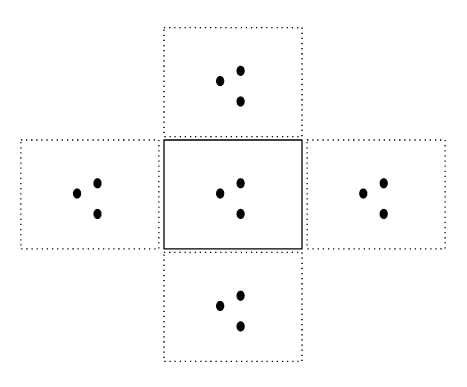
\includegraphics[width=0.7\textwidth]{Figures/pbc}
	\caption{Representation of the periodic boundary condition.}
	\label{fig:pbc}
\end{figure}

The application of the PBC results in particles interacting not only with each other but also with their images. This fact significantly increases the number of interacting pairs and, consequently, the computational time. To overcome that, we need to choose a limited range potential using the minimum image convention criterion. This criterion only allows a particle to interact with the nearest particle or image.  This is technically done during the simulations by neglecting the interactions between two particles at or beyond a maximum length, which is given the name of cutoff radius ($R_{c}$). This cutoff should be equal to or less than half of the box length. This process of examining each pair separation can also be expensive depending on the number of distinct pairs. That is the reason molecular dynamics algorithms use pair listings. This method defines a 'skin' around the cutoff radius with a radius $R_{List}$, as represented in Figure \ref{fig:pairlist}. The pair list is initially built of all the neighbor particles within a distance $R_{List}$ of each particle. Over the course of the simulation, only pairs in the pair list interact. We then will have a list of all particles j with which a particle i interacts as an example. The pair list must then be updated from time to time during the simulation since particles typically diffuse \cite{tuckerman}.    

\begin{figure}[h]
	\centering
	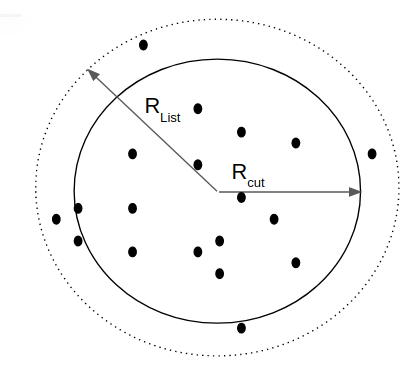
\includegraphics[width=0.5\textwidth]{Figures/pairlist}
	\caption{Representation of the cutoff radius and the pair list radius. Adapted from \citeonline{tuckerman}.}
	\label{fig:pairlist}
\end{figure}

\subsection{Force Fields }
As said previously, we need to calculate the derivative of the potential energy function in relation to the coordinates in order to update the positions during a simulation. Therefore, we need a model for this potential energy functions. These models are called force fields. They can describe structural characteristics such as van der Waals interactions, bond lengths, bond angles, and torsion in a molecular simulation. The description is done by approximating the potential energy function [$U(r^N)$], which has contributions due to intermolecular and intramolecular interactions. The intramolecular interactions include bond stretching, angle bending, and bond torsion. An illustration of these interactions can be seen in Figure \ref{fig:intraint}. 

\begin{figure}[H]
	\centering
	[a]{{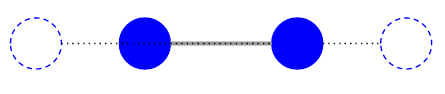
\includegraphics[width=.3\textwidth]{Figures/bondstrech} }}%
	\qquad
	[b]{{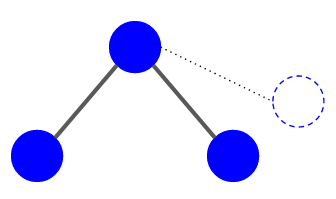
\includegraphics[width=.3\textwidth]{Figures/anglebend} }}%
	\qquad
	[c]{{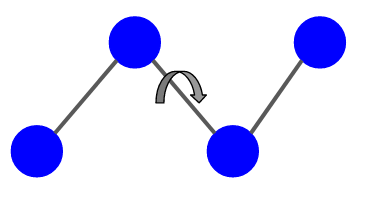
\includegraphics[width=.3\textwidth]{Figures/torsion} }}%    
	\caption{Representation of bond stretching [a], angle bending [b], and bond torsion [c].}%
	\label{fig:intraint}%
\end{figure}


At this dissertation, we are going to present the equations which are most used to represent these interactions. The contribution to the bond stretching (bs ) is usually given by the harmonic approximation around the energy minimum:

\begin{equation}
u_{bs}(d) = k_{bs} (d - d_{0})^2 .
\end{equation}

Here, $d$ is the bond length, $d_{0}$ is the equilibrium bond length, and $k_{bs}$ is a bond stretching constant. The angle bending (ab) contribution corresponds to deviations from the preferred geometry and is often given by:

\begin{equation}
u_{ab}(\theta) = k_{ab} (\theta - \theta _{0})^2,
\end{equation}
where $k_{ab}$ and $\theta _{0}$ are constants defined by the force field and $\theta$ is the bond angle between three atoms.  The bond torsion (bt) interactions correspond to the energies of rotations around bonds, and it happens among four atoms. A commonly used model is

\begin{equation}
u_{bt}(\omega) = \sum_{n=0}^{N}  c_{n} cos^{n} (\omega) ,
\end{equation}
where N is the number of terms, $c_{n}$ is the coefficient defined by the force field, and $\omega$ is the torsional angle also defined by the force field. 

The other type of interactions, the intermolecular interactions or non-bonded interactions, include electrostatic and van der Waals interactions. The first one represents the interaction between two atoms i and j with partial charges ($q_{i}$ and $q_{j}$) and they are usually represented by Coulomb's Law:

\begin{equation}
u_{q}(r_{ij}) = \frac{q_{i}q_{j}}{4 \pi \epsilon _{0} r_{ij}} .
\end{equation} 

In the equation above, $\epsilon _{0}$ is the free space permittivity constant and $r_{ij}$ is the distance between atoms i and j. In many force fields, the van der Waals interaction between particles i and j is modeled by the Lennard-Jones Potential:
\begin{equation}
u_{LJ}(r_{ij}) = 4 \epsilon
\left[ \left(\frac{\sigma}{r_{ij}} \right)^{12} - \left(\frac{\sigma}{r_{ij}} \right)^{6} \right],
\end{equation}
where  $\epsilon$ is the depth of the potential well, $\sigma$ is the distance corresponding to a zero intermolecular potential. The graphical representation of the Lennard-Jones potential is presented in Figure \ref{fig:lj}.
\begin{figure}[H]
	\centering
	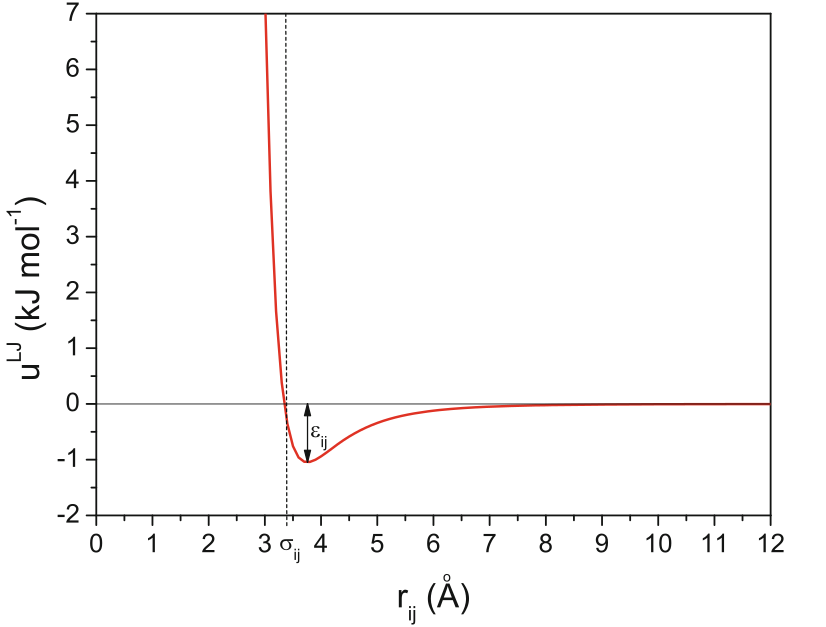
\includegraphics[width=0.8\linewidth]{Figures/lj2}
	\caption{Lennard-Jones potential representation for $\sigma = 1$ and $\epsilon = 1$. }
	\label{fig:lj}
\end{figure}

The potential in Figure \ref{fig:lj} tends to zero and becomes negligible after a specific value of r. Hence, we need to set a cutoff radius in which the potential energy is considered to be zero after it. The point in which the cutoff is defined is generally the one in which the radial distribution function [$g(r)$] is approximately constant. Also, only interactions with the nearest periodic image of the cell are considered for short-range interactions as explained in the Section \ref{icbc}. With this conditions, the calculations of forces and velocities are computationally feasible. The final potential energy function defined by the force field is then expressed by summing all the interactions above:

\begin{equation}
\begin{aligned}
U(r^N) = u_{bs}(d) + u_{ab}(\theta) + u_{bt}(\omega) + u_{q}(r_{ij}) + u_{LJ}(r_{ij}) .
\end{aligned}
\end{equation}
%\subsection{title}
%It is possible to impose movements restrictions on the molecule or even consider the molecule as a rigid body in order to increase the integration step or to follow the modeling of the molecules. Methods for this include the SHAKE, RATTLE and Kamberaj algorithms \cite{RYCKAERT1977327,anderson1983,kamberaj}.

\section{SAFT-$\gamma$ Mie Force Field}


\subsection{SAFT-VR Mie Equation of State (EoS)}

The SAFT-VR Mie equation of state \cite{lafitte2013} is the basis for the SAFT-$\gamma$ Mie coarse-grained force field \cite{avendano2011}, which was the force field used to model the molecules used in the simulations carried out in this dissertation. This EoS was initially developed by \citeonline{lafitte2013} to describe chain molecules formed from fused segments interacting via the Mie attractive and repulsive potential. The Mie potential is a type of generalized Lennard-Jones potential that can be used to explicitly describe repulsive interactions of different hardness/softness and attractive interactions of different ranges, and is given by
\begin{equation}
U_{Mie}(r) = \epsilon\frac{\lambda_r}{\lambda_r - \lambda_a} \left(\frac{\lambda_r}{\lambda_a} \right)^{\left( \frac{\lambda_a}{\lambda_r - \lambda_a} \right)}
\left[ \left(\frac{\sigma}{r} \right)^{\lambda_r} - \left(\frac{\sigma}{r} \right)^{\lambda_a} \right],
\label{eqn:miepotential}
\end{equation}
where $\lambda_r$ is the repulsive exponent and $\lambda_a$ is the attractive exponent. The SAFT-VR Mie equation uses the \citeonline{bh1976} high perturbation expansion of the Helmholtz free energy up to the third order and an improved expression for the  radial distribution function (RDF) of Mie monomers at contact to obtain an equation able to give an accurate theoretical description of the vapor-liquid equilibrium and second derivative properties \cite{lafitte2013}. For a non-associating fluid, the Helmholtz free energy is
\begin{equation}
\frac{A}{N\kappa_{b}T} = a = a^{IDEAL} + a^{MONO} + a^{CHAIN}, 
\label{eqn:miehelm}
\end{equation}
or, depending on the molecule type, the free energy can be equal to
\begin{equation}
\frac{A}{N\kappa_{b}T} = a = a^{IDEAL} + a^{MONO} + a^{RING}.
\label{eqn:miehelmring}
\end{equation}

Here, $a^{IDEAL}$ is the ideal contribution for a mixture. It is given by
\begin{equation}
a^{IDEAL} = \sum_{i=1}^{N_{c}} x_{i}\ln{(\rho_{i}{\Lambda_{i}}^3)} -1 ,
\label{eqn:aideal}
\end{equation}
where $x_{i}=N_{i}/N$ is the molar fraction of component i, $N_{i}$ is the number of molecules of each component, $\rho_{i}=N_{i}/V$ is the number density, and $\Lambda_{i}^3$ is the de Broglie thermal wavelength. Also in Eq. \ref{eqn:miehelm}, $a^{MONO}$ is the monomer contribution, which  describes interactions between Mie segments and can be expressed, for a mixture, as
\begin{equation}
a^{MONO} = \left(\sum_{i=1}^{N_{c}} x_{i}m_{s,i} \right)a^{M} .
\label{eqn:amonomer}
\end{equation}

In the equation above, $m_{s,i}$ is the number of spherical segments making up the molecule i and $a^{M}$  is the monomer dimensionless Helmholtz free energy. $a^{M}$ is expressed as a third-order perturbation expansion in the inverse temperature \cite{bh1976}:
\begin{equation}
a^{M} = a^{HS}+\beta{a_{1}}+\beta{a_{2}}^2+\beta{a_{3}}^3 . 
\label{eqn:aM}
\end{equation}

Here, $a^{HS}$ is the hard-sphere dimensionless Helmholtz free energy for a mixture and is given by:
\begin{equation}
a^{HS} = \frac{6}{\pi\rho_{s}}\left[\left(\frac{\zeta^3_2}{\zeta^2_3}-\zeta_0 \right)\ln(1-\zeta_3)+\frac{3\zeta_{1}\zeta_{2}}{1-\zeta_3}+ \frac{\zeta^3_2}{\zeta_{3}(1-\zeta_3)^2}\right] .
\label{eqn:hs}
\end{equation}

The variable $\rho_{s}=\rho\sum_{i}^{N_c} x_{i}m_{s,i}$ is the total number density of spherical segments and $\zeta_l$ are the moments of the number density:
\begin{equation}
\zeta_l = \frac{\pi\rho_s}{6}\left(\sum_{i=1}^{N_c} x_{s,i}d_{ii} \right), \quad l = 0,1,2,3 ,
\label{eqn:zetal}
\end{equation}
where $x_{s,i}$ is the mole fraction of segments. It is related to the mole fractions of all component ($x_i$) by:
\begin{equation}
x_{s,i} = \frac{m_{s,i}x_i}{\sum_{k=1}^{N_c} m_{s,k}x_{k} } .
\label{eqn:xsi}
\end{equation}


The effective hard-sphere diameter $d_{ii}$ for the segments is
\begin{equation}
d_{ii} =\int_{0}^{\sigma_{ii}} \left \lbrace 1 - \exp \left [-\beta U^{Mie}_{ii}(r) \right ] \right \rbrace dr .
\label{eqn:diameter}
\end{equation}


The integral in Eq. \eqref{eqn:diameter} is normally obtained by means of a 5-point Gauss-Legendre quadrature \cite{papa2014}. For brevity, the detailing of the other terms of Eq. \eqref{eqn:aM} are available at the Appendix \ref{restodaseq}. The term $a^{CHAIN}$ in Eq. \ref{eqn:miehelm} corresponds to the chain contribution. This chain formation of $m_{s}$ tangentially bonded Mie segments is based on the first-order perturbation theory (TPT1)  \cite{papa2014} and can be expressed as
\begin{equation}
a^{CHAIN} =-\sum_{i=1}^{N_{c}} x_{i}(m_{s,i} - 1)\ln \left [ g_{ii}^{Mie}(\sigma_{ii}) \right] .
\label{eqn:achain}
\end{equation}

The term $g_{ij}^{Mie}(\sigma_{ij})$ correspond to the radial distribution function (RDF) of the hypothetical Mie system evaluated at the effective diameter. It is obtained with the following perturbation expansion
\begin{equation}
\begin{aligned}
g_{ij}^{Mie}(\sigma_{ij}) =g_{d,ij}^{HS}(\sigma_{ij})\exp \left [\beta\epsilon \frac{g_{1,ij}(\sigma_{ij})}{g_{d,ij}^{HS}(\sigma_{ij})} + (\beta\epsilon)^{2} \frac{g_{2,ij}(\sigma_{ij})}{g_{d,ij}^{HS}(\sigma_{ij})} \right] .
\end{aligned}
\label{eqn:gmie}
\end{equation}


In the equation above, $g_{d,ij}^{HS}$ is equal to 

\begin{equation}
\begin{aligned}
g_{d,ij}^{HS}(\sigma_{ij}) = \exp (k_{0} + k_{1} x_{0,ij} + k_{2} x_{0,ij}^{2} + k_{3} x_{0,ij}^{3}) ,
\end{aligned}
\label{eqn:ghs}
\end{equation}
where $x_{0,ij} = \sigma_{ij}/d_{ij}$ and $k_{1}, k_{2},$ and $k_{3}$ are density dependent coefficients. These coefficients and the other terms of Eq. \ref{eqn:gmie} are available at Appendix \ref{restodaseq}.  

The ring contribution ($a^{RING}$) in Eq. \ref{eqn:miehelmring} have two forms for rings formed from tangentially bonded segments. The first was developed by \citeonline{lafitte2012}. It considers that the difference between a chain and a ring molecule is that the latter has one more bond that is connecting the first segment to the last. With this assumption, Eq.~\eqref{eqn:achain} can be adapted to rings by
\begin{equation}
a^{RING} =-\sum_{i=1}^{N_{c}} x_{i}m_{s,i}\ln[g_{ii}^{Mie}(\sigma_{ii})] .
\label{eqn:aringlafitte}
\end{equation}

According to \citeonline{lafitte2012}, Eq. \eqref{eqn:aringlafitte} needs an additional parameterization with molecular simulation data so that the EoS can  be used in molecular simulations, but this additional parameterization is not necessary when we are modeling chain molecules. Recently, \citeonline{muller2017} tried to correct this inconsistency. They developed a Helmholtz free energy equation for rings based on the work of \citeonline{muller1993}, who obtained rigorous expressions for hard-sphere fluids with molecular geometries of rings with $m_s=3$. The final expression developed for the dimensionless Helmholtz free energy due to ring formation is
\begin{equation}
a^{RING} =-\sum_{i=1}^{N_{c}} x_{i}\left (m_{s,i}-1+\chi_{i}\eta_{i} \right )\ln \left [g_{ii}^{Mie}(\sigma_{ii}) \right] ,
\label{eqn:aringmuller}
\end{equation}
where $\eta_{i}=m_{s,i}\rho_{i}\sigma_{ii}^{3}/6$ is the packing fraction of the atom i and $\chi_{i}$ is a parameter which depends on $m_{s,i}$ and the geometry of the ring of each component i. For a value of $\chi=0$, Eq. \eqref{eqn:aringmuller} is equal to Eq. \eqref{eqn:achain}. In addition, the equation corresponds to a system of hard sphere triangles when $\chi=1.3827$. \citeonline{muller2017} also calculated values of $\chi$ for $m_{s}=3,m_{s}=4,m_{s}=5$, and $m_{s}=7$ using a geometry formed by a system of equilateral triangles. In these calculations, they used pseudo-experimental data from molecular dynamics (MD) for a defined pure fluid with $\epsilon/\kappa_{b} = 250 K$, $\sigma = 3.0 \dot{A}$, $\lambda_{r} = 11$, and $\lambda_{r} = 6$. Values of $\chi$  for some of the geometry estimated in their article can be seen in \figref{ringqsi}.

\begin{figure}[th]
	\centering
	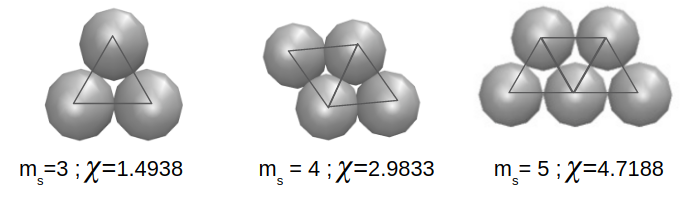
\includegraphics[scale=0.5]{Figures/mullercomtrian}
	\caption{Values for parameter $\chi$ according to the ring geometry. Adapted from \citeonline{muller2017}.}
	\label{ringqsi}
\end{figure}

\citeonline{lafitte2013} also suggested mixing rules for this EoS parameters based on Lorentz-Berthelot combining rules \cite{rowlinson}:
\begin{equation}
\sigma_{ij} =\frac{\sigma_{ii}+\sigma_{jj}}{2},
\label{eqn:sigmamix}
\end{equation}
\begin{equation}
d_{ij} =\frac{d_{ii}+d_{jj}}{2},
\label{eqn:dmix}
\end{equation}
\begin{equation}
\lambda_{k,ij} -3 =\sqrt{(\lambda_{k,ii}-3)(\lambda_{k,jj}-3)},  \quad k=r,a,
\label{eqn:lambdamix}
\end{equation}
\begin{equation}
\epsilon_{ij} =(1-k_{ij})\frac{\sqrt{\sigma_{ii}^{3}\sigma_{jj}^{3}}}{\sigma_{ij}^{3}}\sqrt{\epsilon_{ii}\epsilon_{jj}}.
\label{eqn:epsmix}
\end{equation}

The $k_{ij}$ is a binary interaction parameter to correct the deviations of the mixing rule. This parameter can be described as scaling factor to consider for the interactions among chemically distinct compounds, which are not explicitly accounted by the SAFT-VR Mie EoS. This necessity of an additional parameter raises the question of the quality of these mixing rules and make us wonder if new mixing rules could be used to describe the mixing potential well parameter. Since these were the available mixing rules and the ones employed by other papers that used this force field, we ended up using Eqs. \ref{eqn:sigmamix} to \ref{eqn:epsmix} in our study. However, the binary interaction parameter was only necessary for aqueous mixtures in our study.  


\subsection{Parameter Estimation for the SAFT-$\gamma$ Mie Force Field}\label{parsaft}

The SAFT-$\gamma$ Mie Force Field uses a top-down coarse-graining methodology in its parameterization. This methodology aims to obtain the intermolecular parameters from macroscopic experimental data such as fluid-phase equilibrium or interfacial tension data. The idea is that the force field parameters estimated with the SAFT-VR Mie EoS can be used in molecular simulations since both the equation of state and the force field use the same explicit intermolecular potential model (Mie potential). This correspondence between models has been used to parametrize a variety of fluids \cite{ervik2016}. This force field has the advantage of incorporating the degrees of freedom provided by the use of the Mie Potential \cite{herdes2015}. This flexibility offers the exploration of a vast parameter space without using an iterative simulation scheme \cite{avendano2011}. Despite these advantages, the force field can be restricted by the shortcomings of the equation of state. As an example, the lack of an association term in the equation can cause an inadequate representation of the properties of hydrogen bonding compounds.

Each substance has initially five parameters to be estimated ($m_s,\ \sigma,\ \epsilon,\ \lambda_{r},$ and $, \lambda_{a}$) according to Eq. \eqref{eqn:miepotential}. The number of segments is usually fixed in an integer value since each segment represents one pseudo atom. The attractive parameter is generally  fixed due to its  high correlation with the repulsive parameter. Usually, the chosen value for this parameter is 6, corresponding to the London model, which is a good representation of the dispersion scale of most simple fluids that do not have strong polar interactions \cite{ramrattan2015,herdes2015}. There are two strategies to obtain the parameters: one is by fitting the SAFT-VR Mie EoS to experimental data such as vapor pressure, liquid density and the other one is by using corresponding states parametrization. The first was the one followed in this dissertation. Generally, this approach minimizes the following unweighted least-squares objective function:

\begin{equation}
\begin{aligned}
F_{obj}= \sum_{i=1}^{N_{p}} \left[\frac{P_{v}^{SAFT}(T_{i},\sigma,\epsilon,\lambda_{r})-P_{v}^{exp}(T_{i})}{P_{v}^{exp}(T_{i})} \right]^2 +\\
\sum_{i=1}^{N_{p}} \left[\frac{\rho_{l}^{SAFT}(T_{i},\sigma,\epsilon,\lambda_{r})-\rho_{l}^{exp}(T_{i})}{\rho_{l}^{exp}(T_{i})} \right]^2 ,
\end{aligned}
\label{eqn:fobj}
\end{equation}
where $N_{p}$ is the number of experimental points, $P_{v}$ is the vapor pressure, and $\rho_{l}$ is the saturated liquid density. Other properties that can be used in the estimation are interfacial tension and speed of sound, for instance. The multiple parameters of the model make it necessary the use of a wide range of experimental data since multiple solutions may be found for the fit. Therefore, one needs to be careful in deciding the level of coarse-graining (i.e. the choice of parameter $m_{s}$) and the subsequent parameter space so as to avoid some physical inconsistencies such as a premature freezing \cite{lobanova2015}.

\citeonline{lafitte2012} suggested that two correction factors ($c_{\sigma}$ and $c_{\epsilon}$) should be estimated with simulation data when using Eq. \eqref{eqn:aringlafitte} for the ring contribution. They are related to the EoS parameters by scaled parameters:

\begin{equation}
\sigma^{scaled} = c_{\sigma}\sigma^{SAFT}.
\label{eqn:csigma}
\end{equation}
\begin{equation}
\epsilon^{scaled} = c_{\epsilon}\epsilon^{SAFT}.
\label{eqn:ceps}
\end{equation}

According to \citeonline{lafitte2012}, these corrections are necessary because the approximations employed in the EoS theory generate discrepancies between molecular simulations and the EoS for ring molecules modeled with Eq. \eqref{eqn:aringlafitte}. However, this new parameterization is not necessary when using Eq. \eqref{eqn:aringmuller} as the ring contribution or when we are modeling chain molecules with Eq. \ref{eqn:achain}. This fact makes the strategy of \citeonline{lafitte2012} inconsistent since parameterization with molecular simulation should not be necessary according to the overall idea of this force field. Furthermore, the use of molecular simulation data highly increases the time spent on the parameterization process. The objective function for the estimation of the correction parameter is given by

\begin{equation}
\begin{split}
F_{obj}= \sum_{i=1}^{N_{p}} \left[\frac{P_{v}^{sim}(T_{i},\sigma^{SAFT},\epsilon^{SAFT})-P_{v}^{SAFT}(T_{i},\sigma^{scaled},\epsilon^{scaled})}{P_{v}^{sim}(T_{i},\sigma^{SAFT},\epsilon^{SAFT})} \right]^2 + \\
\sum_{i=1}^{N_{p}} \left[\frac{\rho_{liq}^{sim}(T_{i},\sigma^{SAFT},\epsilon^{SAFT})-\rho_{liq}^{SAFT}(T_{i},\sigma^{scaled},\epsilon^{scaled})}{\rho_{liq}^{sim}(T_{i},\sigma^{SAFT},\epsilon^{SAFT})} \right]^2 .
\end{split}
\label{eqn:fobjla}
\end{equation}

The repulsive parameter is maintained in the value found on the minimization of Eq. \eqref{eqn:fobj}. The refined values for $\sigma$ and $\epsilon$ are

\begin{equation}
\sigma^{sim} = \sigma^{SAFT}/c_{\sigma},
\label{eqn:simsigma}
\end{equation}

\begin{equation}
\epsilon^{sim} = \epsilon^{SAFT}/c_{\epsilon},
\label{eqn:simeps}
\end{equation}

The other method to obtain the force field parameters is the corresponding states parametrization \cite{mejia2014}. This method considers that the unweighted volume average of the attractive contribution to the Mie intermolecular potential, $ \, a_{1}$, is the following mean-field approximation

\begin{equation}
a_{1} = 2\pi\rho\sigma^{3}\epsilon\alpha .
\label{eqn:a1corres}
\end{equation}

The van der Waals constant, $\alpha$, considering $ \lambda_{a} = 6$ is related by the Mie exponents by

\begin{equation}
\alpha = \frac{1}{\epsilon\sigma^{3    }} \int_{\sigma}^{\infty} \phi(r)r^{2}dr = \frac{\lambda_{r}}{3(\lambda_{r}-3)}\left(\frac{\lambda_r}{6}\right)^{6/(\lambda_{r} - 6)}  .
\label{eqn:alpha}
\end{equation}

The parameterization in this method starts by using the experimental acentric factor, $\omega$, for each molecule with a fixed value of $ m_{s}$ to obtain the value of the repulsive exponent with the following Padé series:

\begin{equation}
\lambda_{r} = \frac{\sum_{i=0} a_{i}\omega^{i}}{1+\sum_{i=1} b_{i}\omega^{i}} ,  
\label{eqn:lambdaco}
\end{equation}
where $a_{i}$ and $b_{i}$ are parameters that are dependent on the number of segments. A table with these parameters is presented in the original paper \cite{mejia2014}. The van der Waals constant can be found by substituting $\lambda_{r}$ into Eq. \eqref{eqn:alpha}. The reduced critical temperature $T_{c}^{*}$ is related to $\alpha$ by a Padé series: 

\begin{equation}
T_{c}^{*} = \frac{\sum_{i=0} c_{i}\alpha^{i}}{1+\sum_{i=1} d_{i}\alpha^{i}}   .
\label{eqn:tc}
\end{equation}

The values of $c_{i}$ and $d_{i}$ are also available in the original paper. The reduced temperature of the equation above is used in conjunction with the experimental critical temperature, $ T_{c}$, to find the energy parameter with the relation below:

\begin{equation}
T_{c}^{*} = \frac{\kappa_{b}T_{c}}{\epsilon}   .
\label{eqn:epscorre}
\end{equation}

The diameter parameter, however, is not obtained with the critical properties, but with the reduced liquid density at the reduced temperature of $0.7$ ($\rho_{T_{r}=0.7}$). This density is also obtained with a Padé series using parameters by \citeonline{mejia2014}:

\begin{equation}
\rho_{T_{r}=0.7}^{*} = \frac{\sum_{i=0} j_{i}\alpha^{i}}{1+\sum_{i=1} k_{i}\alpha^{i}} .
\label{eqn:denscorre}
\end{equation}

The relation between the equation above, $\sigma$ and the experimental density is given by

\begin{equation}
\rho_{T_{r}=0.7}^{*} = \rho_{T_{r}=0.7}\sigma^{3}N_{av},   
\label{eqn:sigmacorre}
\end{equation}
where $N_{av}$ is the Avogadro number. This corresponding states method has the advantage of only requiring critical data, which is available for a great range of fluids, and liquid density data. The parameters of a variety of compounds for this force field are available at a large online database available at: http://www.bottledsaft.org \cite{ervik2016}. Hence, here, we only expose the coarse-grained geometries and the sets of parameters for the compounds used in this work. They are available  at Tables \ref{tbl:geopara} and \ref{tbl:parameters}. The parameters for water were retrieved from \citeonline{lobanova2016}; for carbon dioxide, propane, and hexane from \citeonline{herdes2015}; for 1-octanol from \citeonline{ervik2016}; and for the aromatic compounds from   \citeonline{muller2017}.     

\begin{table}[h]
	\caption{Coarse-grained geometries of the substances used in this work for the SAFT-$\gamma$ Mie.}
	\centering
	\label{tbl:geopara}
	\begin{tabular}{ccc}
		
		\toprule \toprule
		Molecule &  Structure &  Coarse grained structure  \\
		\midrule \midrule
		Water &
		\adjustimage{height=1.2cm,valign=m}{Figures/waterg} &
		\adjustimage{height=1cm,valign=m}{Figures/onebead}  \\
		Carbon dioxide &
		\adjustimage{height=0.8cm,valign=m}{Figures/co2g} &
		\adjustimage{height=1cm,valign=m}{Figures/twobeads}  \\
		Propane & \adjustimage{height=1.5cm,valign=m}{Figures/propg}  & \adjustimage{height=1cm,valign=m}{Figures/onebead} \\
		Hexane & \adjustimage{height=1.5cm,valign=m}{Figures/hexg}  & \adjustimage{height=1cm,valign=m}{Figures/twobeads} \\
		1-octanol & \adjustimage{height=1.5cm,valign=m}{Figures/octg}  & \adjustimage{height=1cm,valign=m}{Figures/threebeads} \\
		Toluene & \adjustimage{height=2.5cm,valign=m}{Figures/tolg}  & \adjustimage{height=2cm,valign=m}{Figures/fe3} \\
		Benzene & \adjustimage{height=2.5cm,valign=m}{Figures/benzg}  & \adjustimage{height=2cm,valign=m}{Figures/fe3} \\
		Pyrene & \adjustimage{height=2.5cm,valign=m}{Figures/pyre}  & \adjustimage{height=2cm,valign=m}{Figures/pyrecg} \\
		Anthracene & \adjustimage{height=2cm,valign=m}{Figures/ant}  & \adjustimage{height=2cm,valign=m}{Figures/fen5} \\
		\bottomrule \bottomrule
		
	\end{tabular}
\end{table}

\begin{table}[h]
	\centering
	\caption{Parameters of the SAFT-$\gamma$ Mie force field for each substance used in this work.}
	\label{tbl:parameters}
	\begin{tabular}{ccccc}
		\hline
		\hline
		& $m_s$ & $\epsilon/\kappa_{b}$ (K) & $\sigma$ (\AA) & $\lambda_r$ \\ \hline\hline
		Water          & 1     & 305.21               & 2.902              & 8.0         \\
		Carbon dioxide & 2     & 194.94               & 2.848              & 14.65       \\
		Propane        & 1     & 426.08               & 4.871              & 34.29       \\
		Hexane         & 2     & 376.35               & 4.508              & 19.57       \\
		1-octanol        & 3     & 495.71               & 4.341              & 28.79       \\
		Toluene        & 3     & 268.24               & 3.685              & 11.80       \\
		Benzene        & 3     & 230.30               & 3.441              & 10.45       \\
		Pyrene         & 4     & 459.04               & 4.134              & 15.79       \\
		Anthracene     & 5     & 259.68               & 3.631              & 9.55        \\ 
		\hline
		\hline
	\end{tabular}
	
\end{table}
\FloatBarrier
The binary interaction parameter $k_{ij}$ of Eq. \eqref{eqn:epsmix} is normally estimated by minimizing the difference between experimental binary vapor-liquid equilibrium or interfacial tension data and the SAFT-VR Mie EoS output data \cite{muller2017,lobanova2016}. The objective function is similar to: 

\begin{equation}
\begin{aligned}
F_{obj}= \sum_{k=1}^{N_{p}} \left(\frac{P_{v}^{SAFT}(T_{k},x,k_{ij})-P_{v}^{exp}(T_{k},x)}{P_{v}^{exp}(T_{k},x)} \right)^2 +\\
\sum_{k=1}^{N_{p}} \left(\frac{\rho_{l}^{SAFT}(T_{k},x,k_{ij})-\rho_{l}^{exp}(T_{i})}{\rho_{l}^{exp}(T_{i})} \right)^2 .
\end{aligned}
\label{eqn:fobjmix}
\end{equation}

However, \citeonline{ervik20162} used molecular simulation results to fit the parameter to the interfacial tension data. The strategy they followed was to carry out simulations in three values of $k_{ij}$ first and, after, refine the parameter until a value in good agreement with the experimental data is found. We decided to follow this strategy in our estimations of $k_{ij}$ since the estimation with the EoS did not provide satisfactory results for the hydration free energy calculations.  


\section{Solvation Free Energy Calculations Based on Molecular Dynamics}
% background topics

Using the SAFT-$\gamma$ Mie Force Field described in the section above, we carried out solvation free energy molecular dynamics simulations. The free energies we are trying to calculate can be expressed as averages over ensembles of atomic configurations generated using Monte Carlo or Molecular Dynamics techniques. In the canonical ensemble, the free energy is given by  

\begin{equation}
\label{eq:fcano}
\begin{aligned}
F(N,V,T) = -\kappa_{b}T \ln Q(N,V,T).
\end{aligned}
\end{equation}

Recall that $Q(N,V,T)$ is the partition function of the canonical ensemble, expressed as

\begin{equation}
\label{eq:partican}
\begin{aligned}
Q(N,V,T) =\frac{\epsilon_{0}}{h^{3N}N!} \int d^{n}p d^{n}r \exp \left[ -\beta \left( \sum_{i=1}^{N}\dfrac{p_{i}^{2}}{2m_{i}} + U(r_{1},..,r_{n}) \right)
\right] .
\end{aligned}
\end{equation}

The Gibbs free energy, the object of study in this dissertation, is given by

\begin{equation}
\begin{aligned}
G(N,P,T) = -\kappa_{b}T ln \Delta (N,P,T),
\end{aligned}
\end{equation}
where $\Delta (N,P,T)$ is the partition function of the isothermal-isobaric ensemble:

\begin{equation}
\begin{aligned}
\Delta (N,P,T) = \frac{1}{V_{0}} \int_{0}^{\infty} dV \int d^{n}p d^{n}r \exp \left[ -\beta \left( \sum_{i=1}^{N}\dfrac{p_{i}^{2}}{2m_{i}} + U(r_{1},..,r_{n}) + PV(r_{1},..,r_{n}) \right) \right].
\end{aligned}
\end{equation}

Evaluating the partition function is an often unfeasible task, but we are interested in calculating only the Gibbs free energy difference between two states of a system, which is  

\begin{equation}
\begin{aligned}
\Delta G_{AB} = G_{B} - G_{A}= -\kappa_{b}T ln \left( \frac{\Delta_{B}}{\Delta_{A}}\right) .
\end{aligned}
\end{equation}

Since the masses of particles in states A and B of a system are the same and the Hamiltonian is separable in $K(p)$ and $U(r)$, the moment integrals in the ratio ${\Delta_{B}}/{\Delta_{A}}$ can be simplified into the ratio of the configuration integrals:

\begin{equation}
\label{eq:partiso}
\begin{aligned}
\dfrac{Z_{B}}{Z_{A}} = \dfrac{\int_{0}^{\infty} dV \int d^{n}r \exp \left\lbrace -\beta \left[U(r_{1},..,r_{n}) + PV(r_{1},..,r_{n}) \right]_{B} \right\rbrace}{\int_{0}^{\infty} dV \int d^{n}r \exp \left\lbrace  -\beta \left[U(r_{1},..,r_{n}) + PV(r_{1},..,r_{n}) \right]_{A} \right\rbrace }.
\end{aligned}
\end{equation}

This identity results in the following equation for the Gibbs free energy difference, which does not  require the calculation of the partition function at each state:

\begin{equation}
\label{eq:dif}
\begin{aligned}
\Delta G_{AB} = G_{B} - G_{A}= -\kappa_{b}T ln \left( \frac{Z_{B}}{Z_{A}}\right).
\end{aligned}
\end{equation}

In the case of a study concerning the solvation of a single molecule, the Gibbs free energy difference between end states $A$ and $B$ are, more specifically, the difference between the solute alone in the gas phase and the solute interacting with the solvent. In order to have accurate results for free energy differences, the states need to have sufficient overlap  \cite{klimovich}. The overlap can be achieved by calculating the free energy difference among a series of intermediates states. The result of these differences is independent of the path chosen since free energy is a state function. That is why alchemical states (without physical sense) can be used to link physical states of interest. The solvation free energy calculations are then done through a thermodynamic path in which the solute molecule is gradually inserted into the solvent as illustrated in \figref{thermcy}. According to this path, the free energy of solvation is expressed as

\begin{equation}
\label{eq:freesolv}
\begin{aligned}
\Delta G_{solv} = \Delta G_{1 \rightarrow 4} = \Delta G_{1 \rightarrow 2} + \Delta G_{2 \rightarrow 3} + \Delta G_{3 \rightarrow 4}  - \kappa_{b}T \ln \dfrac{V^{*}}{V^{1}} .
\end{aligned}
\end{equation}

\begin{figure}[th]
	\centering
	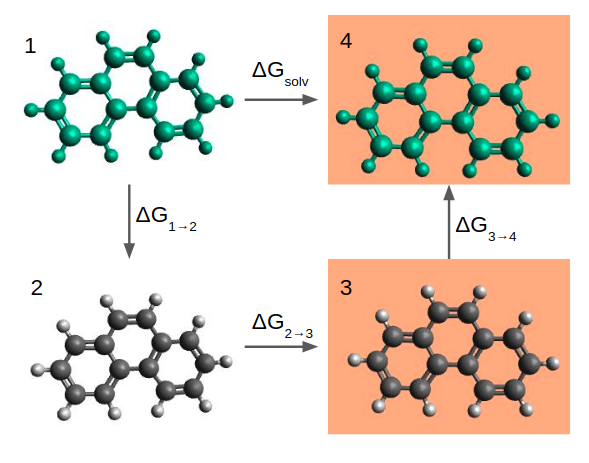
\includegraphics[scale=0.6]{Figures/cicclotermo}
	\caption{Thermodynamic path for computing solvation free energy of a single solute molecule with molecular dynamics. Adapted from \citeonline{klimovich}.}
	\label{thermcy}
\end{figure}

The last term in Eq. \ref{eq:freesolv} accounts for the difference between the mean volume of the simulation box with the solute inserted ($V_{1}$) and the mean volume of the simulation box with only solvent molecules in it ($V^{*}$). However, \citeonline{shirts2013} have shown that this term is negligible with respect to the statistical uncertainty of calculating $\Delta G$. In addition, when we have other solute molecules that are equal to the solute molecule being inserted in the box, another term in Eq. \ref{eq:freesolv} can appear in order to distinguish these molecules \cite{shirts2013}. The  term $\Delta G_{1 \rightarrow 2}$, also represented in \figref{thermcy},  is the solvation free energy associated with turning off the non bonded interactions of the molecule in the gas phase. In the next transformation, $\Delta G_{2 \rightarrow 3}$ is the free energy of moving the non-interacting molecule from the gas phase to the solvent and is equal to zero since the transformation of a non-interacting molecule does not depend on the environment. Lastly, $\Delta G_{3 \rightarrow 4}$ is the free energy required for the non-interaction molecule in the solvent phase to regain its non-bonded interactions with the solvent.  The solvation free energy calculation can be classified according to the types of non-bonded interactions that are turned off/on in the $1 \rightarrow 2$ and $ 3 \rightarrow 4$ parts of the path. If both non-bonded interactions with the environment and internal interactions are turned off, this is an annihilation free energy calculation. On the other hand, if only non-bonded interactions with the environment are turned off, this is a decoupling free energy calculation \cite{klimovich}. In the latter case, $\Delta G_{1 \rightarrow 2} = 0$ and the $\Delta G_{solv} = \Delta G_{3 \rightarrow 4} $.  

The methods used to carry out the transformations of Figure \ref{thermcy} during the simulation scale the solute charges to zero and then turn off the interactions corresponding to the Lennard-Jones or Mie potential. In order to carry out the latter process, a modified potential with a coupling parameter ($\lambda$) is used. Each $\lambda$ represents an alchemical state. When $\lambda=0$, there is no interaction with the solvent and, when $\lambda=1$, interactions are fully activated. The coupling of the $\lambda$ parameter could be linear, as it is demonstrated in Figure \ref{fig:linearpoten}, but it could generate numerical problems related to the exponential part of the potential \cite{shirts2013}. 

\begin{figure}[H]
	\centering
	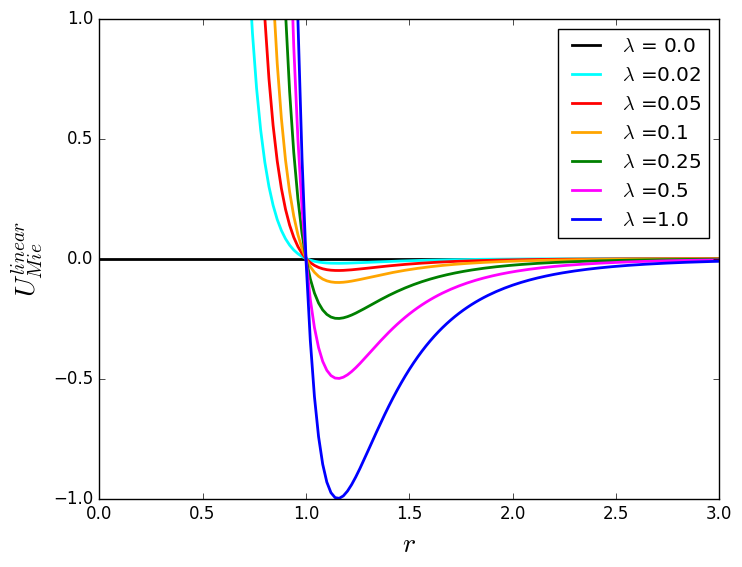
\includegraphics[width=0.8\linewidth]{Figures/linear8}
	\caption{Linear coupling of the potential energy, $U^{linear}_{Mie} = \lambda U_{Mie}$, for different values of $\lambda$. Here, $\sigma=1$, $\epsilon=1$, $\lambda _a = 6$, and $\lambda _r = 8$.}
	\label{fig:linearpoten}
\end{figure} 

Observing Figure \ref{fig:linearpoten}, we can see that a linear coupling of the parameter would cause an abrupt change in the potential energy when the $\lambda$ reaches zero. That is the reason the non-linear softcore scheme \cite{beutler1994} is used to couple the $\lambda$. This scheme makes the potential behave more smoothly in relation to the change of $\lambda$. 

The softcore potential is equal to

\begin{equation}
\label{eq:softcoreLJ}
\begin{aligned}
U_{LJ}^{sc}(r) {}=& 4\lambda\epsilon \left\lbrace\frac{1}{\left[\alpha(1-\lambda)+ (r/\sigma)^{6}\right]^{2}} - \frac{1}{\alpha(1-\lambda)+(r/\sigma)^{6}}\right\rbrace ,
\end{aligned}
\end{equation}
where $\alpha$ is a constant whose value is  normally assumed to be 0.5.    Based on Eq. \ref{eq:softcoreLJ}, we propose a generalized softcore Mie potential for any value of $\lambda _{r}$ and $\lambda _{a}$. It is given by:

\begin{equation}
\label{eq:softcore}
\begin{aligned}
U^{sc}(r) {}=& \lambda\epsilon\dfrac{\lambda_r}{\lambda_r - \lambda_a} \left(\frac{\lambda_r}{\lambda_a} \right)^{\left( \frac{\lambda_a}{\lambda_r - \lambda_a} \right)} \left\lbrace\dfrac{1}{\left[\alpha(1-\lambda)+ (r/\sigma)^{\lambda_a}\right]^{\lambda_{r}/\lambda_{a}}} - \dfrac{1}{\alpha(1-\lambda)+(r/\sigma)^{\lambda_a}}\right\rbrace .
\end{aligned}
\end{equation}

Using this generalized softcore potential, we plotted the relation between the values of $\lambda$ and the potential for repulsive exponents of different hardness/softness in Figure \ref{fig:scmie}. We see that this softcore scheme makes the potential behave more smoothly in relation to the change of $\lambda$, mainly for the smaller repulsive exponents. 
 

\begin{figure}%
	\centering
	\subfloat[][]{%
		\label{fig:ex3-a}%
		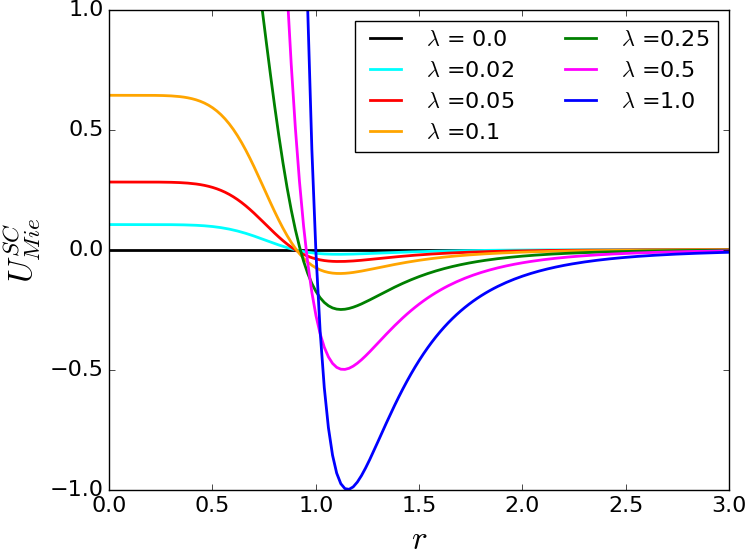
\includegraphics[height=5.9cm]{Figures/soft8}}%
	\hspace{0.05cm}%
	\subfloat[][]{%
		\label{fig:ex3-b}%
		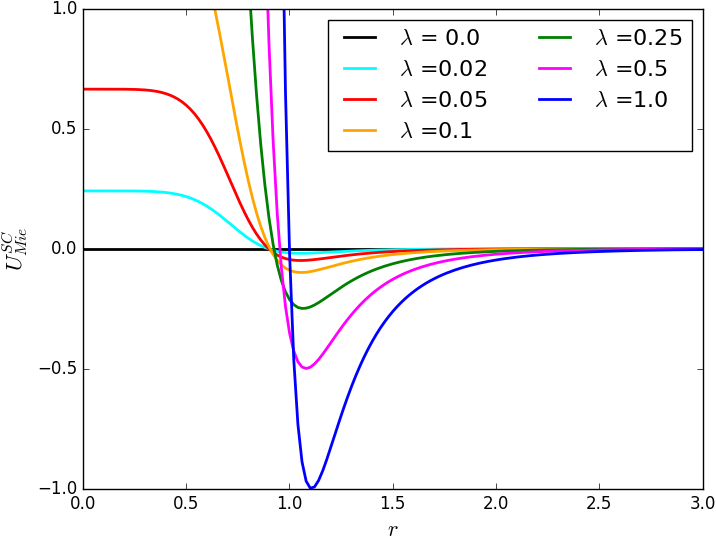
\includegraphics[height=5.9cm]{Figures/soft15}} \\

	\subfloat[][]{%
		\label{fig:ex3-c}%
		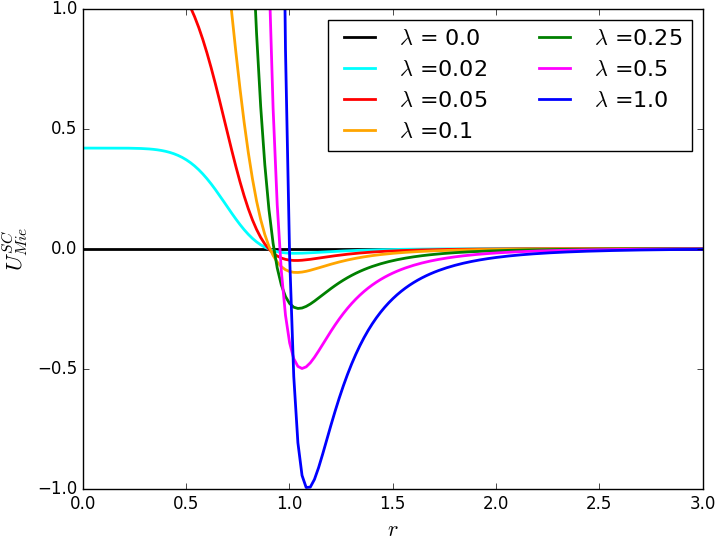
\includegraphics[height=5.9cm]{Figures/soft20}}%
	\hspace{0.05cm}%
	\subfloat[][]{%
		\label{fig:ex3-d}%
		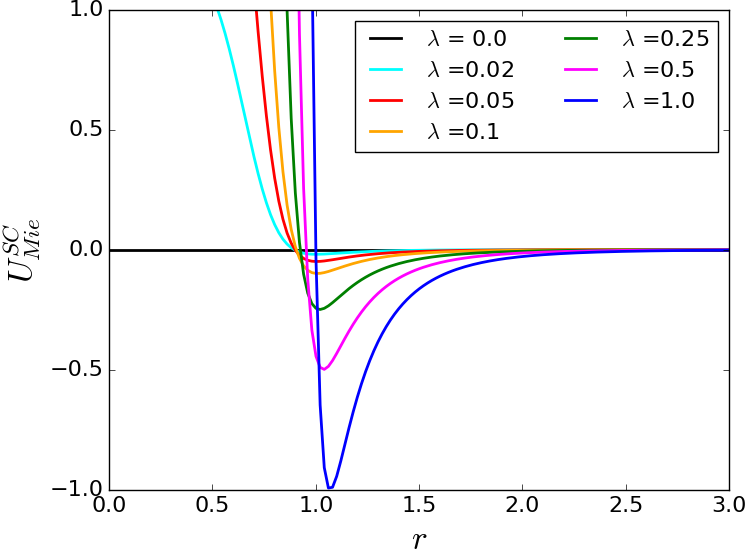
\includegraphics[height=5.9cm]{Figures/soft30}}%
	\caption[Generalized softcore Mie potential, Eq. \ref{eq:softcore}, for different values of $\lambda$.]{Generalized softcore Mie potential, Eq. \ref{eq:softcore}, for different values of $\lambda$. Here, $\sigma=1$, $\epsilon=1$, $\lambda _{a} = 6$, and $\lambda _{r}$ is equal to
		8 \subref{fig:ex3-a};
		15 \subref{fig:ex3-b};
		20 \subref{fig:ex3-c}; and,
		30 \subref{fig:ex3-d}.}%
	\label{fig:scmie}
\end{figure}

Now that we defined our coupled potential, we can then obtain the potential energies related to each alchemical state by doing independent simulations in different values of $\lambda$ or by doing expanded ensemble simulations \cite{lyubartsev}. The latter was the method used in this dissertation, and it is described in Section \ref{ee}. With the potential energies, the next step is to use post-processing methods, such as the MBAR used in this study, to effectively calculate $\Delta G_{3 \rightarrow 4}$.  The solvation free energies can then be used to calculate other properties such as the partition coefficient. This property is a measure of the partitioning of one solute in two solvents (a and b) with different physicochemical characteristics  at a temperature T. It is defined by the following equation when the activity coefficients are assumed to be one \cite{doi:10.1021/ja00036a009}:

\begin{equation}
P = \dfrac{[solute]_{a}}{[solute]_{b}},
\end{equation} 
where $[solute]_{a}$ and $[solute]_{b}$ are the concentration of the solute in the solvent a and b, respectively. Since $P$ is an equilibrium constant, it can be related to free energy change associated with transferring the solute from the phase a to the phase b. Hence, we can define the relation between the partition coefficient and the difference in free energy with the equation bellow \cite{doi:10.1021/ja00036a009}:  

\begin{equation}
\label{eqn:partcoe}
{2.303RT} \log{P}^{a/b} ={\Delta G_{solv}^{a} - \Delta G_{solv}^{b}},
\end{equation}
where 2.303 is a conversion factor.

\section{Expanded Ensemble Method}\label{ee}

We decided to use the Expanded Ensemble method \cite{lyubartsev} in our solvation free energy simulations since it allows a non-Boltzmann sampling scheme of different states in a single simulation. \citeonline{lyubartsev} initially proposed in their paper a sampling scheme of different temperatures, but this idea can be generalized to a sampling scheme of different states or $\lambda 's$ \cite{escobedo2007}. In this scheme, the sampling is done by biasing the phase space exploration process with weights not related to the statistical ensemble. The partition function of the statistical expanded ensemble, $Z^{EE}$, is obtained from the probability distributions corresponding to each $\lambda$. Hence, $Z^{EE}$ is defined as a sum of subensembles $Z_{i}$ in different values of $\lambda$, that is,

\begin{equation}
Z^{EE} = \sum_{i=1}^{N} Z_{i}(\lambda_{i}) exp(\eta_{i}),
\label{eqn:ee}
\end{equation}   
where N is the number of alchemical states, $\eta_{i}$ is the arbitrary weight of the subensemble at each state, and $Z_{i}$ is the configurational partition function of state i. For the isothermal-isobaric ensemble, $Z_{i}$ is given by

\begin{equation}
Z_{i} = \frac{1}{V_{0}} {\int_{0}^{\infty} dV \int d^{n}r^{n} \exp \left \lbrace -\beta_{i} \left[ U(\lambda, r_{1},..,r_{n}) + P_{i}V(r_{1},..,r_{n}) \right] \right \rbrace}.
\end{equation} 

In solvation free energy calculations with molecular dynamics, $\lambda$ corresponds to the coupling parameter of the softcore potential (Eq. \ref{eq:softcoreLJ}). Since we are carrying out molecular dynamic simulations, the sampling of the expanded ensemble is done by performing an arbitrary number of MD  steps followed by a $\lambda$ transition. \citeonline{chodera2011} proved that this type of sampling of the expanded ensemble is similar to the Gibbs sampling method \cite{geman1984,liu2002}. Following the Gibbs method, the sampling of the configuration space $x$ for one state $\lambda_{k}$ during the MD steps is done by using the conditional distribution:

\begin{equation}
\pi(x|\lambda_{k}) = \dfrac{\exp[-\beta u(x,\lambda_{k})]}{\int dx \exp [- \beta u(x,\lambda_{k})]}.
\label{eqn:rhoee1}
\end{equation} 

The state transition in the MD simulation uses the following conditional distribution:

\begin{equation}
\pi(\lambda_{k}|x) = \dfrac{\exp[-\beta u(x,\lambda_{k}) + \eta_{k}]}{ \sum_{k=1}^{K} \exp [- \beta u(x,\lambda_{k})+ \eta_{k}]},
\label{eqn:rhoee2}
\end{equation} 
where $u(x,\lambda_{k})$ is the reduced potential function for the NPT ensemble. There is a variety of acceptance schemes to do the expanded sampling using Eq. \eqref{eqn:rhoee2}, but \citeonline{chodera2011} suggested that the independence sampling \cite{liu2002} is the best strategy to increase the number of uncorrelated configurations. The implementation they suggested consists of updating the state index from $i$ to $j$ by first generating a uniform random number $R$ on the interval $[0,1)$ and then selecting the smallest new value of $j$ that satisfies  the relation

\begin{equation}
R < \sum_{i=1}^{j} \pi(\lambda_{i}|x) .
\label{eqn:relee2}
\end{equation} 

The sampling strategy above depends on a proper selection of weights in order to guarantee an adequate sampling of the states. If there is not a sufficient number of visits to each state, the expanded ensemble becomes deficient in obtaining input data to estimate free energy differences with the methods exposed in Section \ref{SFECM}. Here, we followed the flat-histogram approach \cite{bernd1992,bernd1993,dayal2004} to calculate the weights. This strategy aims to obtain adequate sampling by ensuring that all the states have an equal number of visits, i.e. the ratio of the probability of sampling state i ($\pi_{i}$) to the probability of sampling state $j$ ($\pi_{j}$) is equal to one. Given that $\pi_{i}$ is equal to:

\begin{equation}
\pi_{i} = \dfrac{Z_{i}(\lambda_{i}) exp(\eta_{i})}{Z^{EE}} ,
\label{eqn:wei1}
\end{equation} 
and using Eqs. \ref{eq:dif} and \ref {eq:partiso}, the following relation can be obtained for $\pi_{i}/\pi_{j}=1$:

\begin{equation}
(\eta_{i} - \eta_{j}) = \beta(G_i-G_j).
\label{eqn:weight}
\end{equation}

Eq. \eqref{eqn:weight} proposes that the choice of the weights is dependent on the free energies that we are attempting to obtain. This equation is then solved iteratively with trial simulations. For the first simulation, the values of $\eta$ are set to zero, and the histogram of the states visited is obtained. With this histogram, it is possible to estimate the free energy differences and, since the weights are related to the free energies by Eq. \eqref{eqn:weight}, the next values of $\eta$ can be calculated. This iteration goes on until a uniform distribution is attained. The weights found are then used in a longer simulation to obtain the final solvation free energies.

The choice of the $\lambda$ set corresponding to overlapping alchemical states are crucial to acquire accurate solvation free energies. In this work, the method chosen to obtain the optimal staging of the $\lambda$ domain is the one developed by \citeonline{escobedo2007} with a basis in the study of  \citeonline{1742-5468-2006-03-P03018}. This method targets "bottlenecks" in the simulation. It does that by optimizing $\lambda$ through the minimization of the number of round trips per CPU time between the lowest ($0$) and highest ($1$) values of $\lambda$. This is specifically done by maximizing the steady-state flow $\phi$ of the simulation, which "walks" among the values of $\lambda$. This flow is estimated from a Fick's diffusion type of law:

\begin{equation}
\phi = D(\Lambda) \Pi (\Lambda) \dfrac{dx(\Lambda)}{d \Lambda}.
\label{eqn:stream}
\end{equation}

In the equation above, $\Lambda$ is the actual continuous value of the coupling parameter. This continuous function of $\lambda 's$ is obtained by interpolating the $\lambda$ set linearly. $D(\Lambda)$ is the diffusivity at  state $\Lambda$ and $x(\Lambda)$ is the fraction of times that the trial simulation at state $\Lambda_{i}$ has most recently visited the state $\lambda=1$ as opposed to state $\lambda=0$. The derivative ${dx(\Lambda)}/{d \Lambda}$ is approximated with the central finite differences method. Finally, $\Pi (\Lambda)$ is the probability of visiting $\Lambda$:

\begin{equation}
\Pi (\Lambda) = \dfrac{C^{'} \bar{\Pi} (\lambda)}{\Lambda_{i+1} - \Lambda_{i}}.
\label{eqn:plambda}
\end{equation}

The $C^{'} $ term in the equation above represents a constant and $\bar{\Pi} (\lambda)$ is the arithmetic average of the frequency of visits to the $\Lambda$ state:

\begin{equation}
\bar{\Pi}_{i} (\lambda) = \dfrac{\pi_{i+1} - \pi_{i}}{2}.
\label{eqn:barplambda}
\end{equation}

The $\phi$ is maximum when the optimal probability $\Pi^{'}(\Lambda_{i})$ of visiting state $\Lambda_{i}$ is proportional to $1/\sqrt{D(\Lambda)}$ \cite{trebst2004}. With that information, it is possible to estimate the diffusivity using one trial simulation with the following equation:

\begin{equation}
\begin{aligned}
D(\Lambda) {}=& \dfrac{\Lambda_{i+1} - \Lambda_{i}}{\bar{\Pi} (\lambda) {dx(\Lambda)}/{d \Lambda}}, \quad \Lambda_{i} < \Lambda < \Lambda_{i+1}.
\end{aligned}
\label{eqn:diff}
\end{equation}    
Hence, we can calculate $\bar{\Pi} $ and, consequently, the cumulative probability, which is used to obtain the new $\lambda$ states by

\begin{equation}
\Phi = \int_{\lambda =0}^{\lambda =1} \Pi^{'}(\Lambda_{i}) d \Lambda = \dfrac{i}{K},
\label{eqn:cumfun}
\end{equation}
where $K$ is the total number of $\lambda$ states. In order to carry out our solvation free energy simulations, we obtained these cumulative probabilities for every $\lambda$ set we estimated. A graphical demonstration of the relation between the optimized coupling parameters and the cumulative probability of Eq. \ref{eqn:cumfun} is presented in Figure \ref{fig:optimized_cdfexeample}.

\begin{figure}[h]
	\centering
	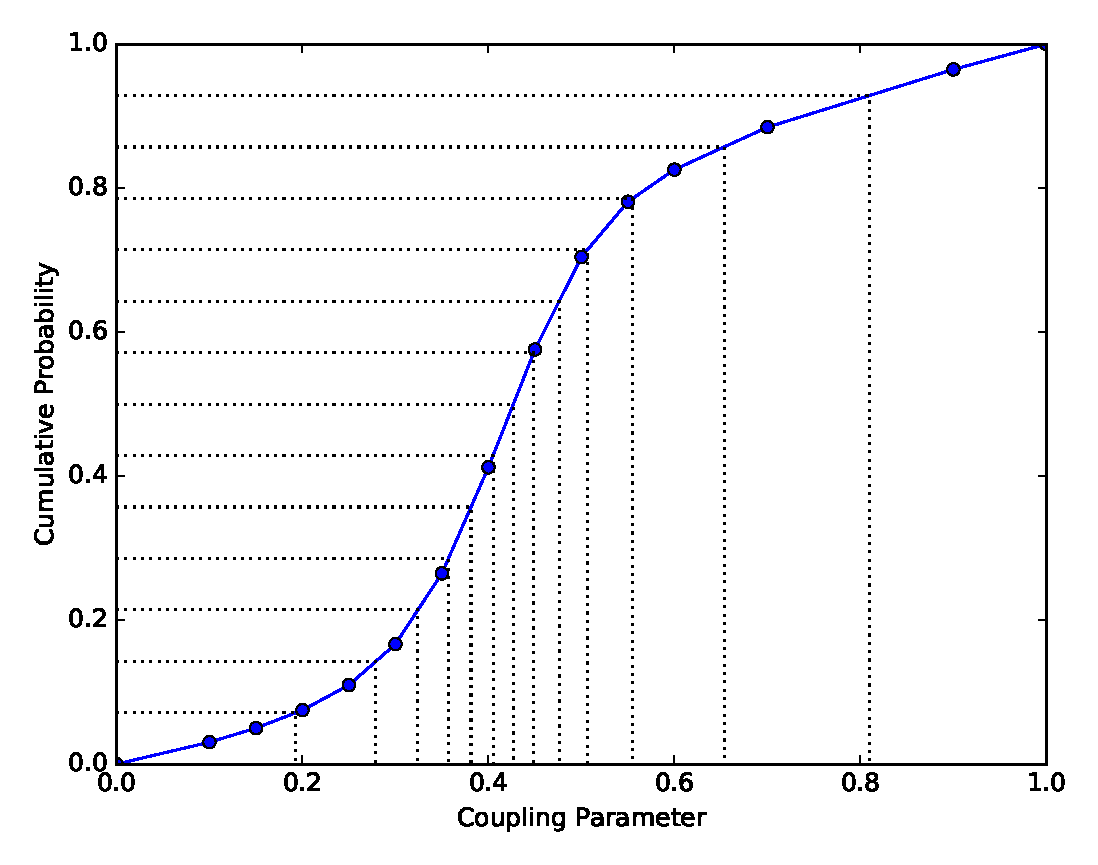
\includegraphics[width=0.8\linewidth]{Figures/optimized_cdfexeample}
	\caption{Relation between the optimized coupling parameters and the cumulative probability used to obtain them.}
	\label{fig:optimized_cdfexeample}
\end{figure}
\FloatBarrier
\section{Multistate Bennett Acceptance Ratio (MBAR)}\label{mbar}

We presented in the sections above the methods used to obtain the total potential energies of each alchemical state with molecular dynamics, and, in this section, we are going to discuss the methodology utilized to estimate the solvation free energies with these data. The MBAR method \cite{mbar} is based on the free energy perturbation. It is a maximum likelihood method which computes free energies and their uncertainties of all $K$ states by minimizing the $K \times K$ matrix of variances for a simulation with $N_{j}$ uncorrelated samples in equilibrium. For each of the $\lbrace x_{i,n } \rbrace ^{N_{i}}_{n=1 }$ configurations of i, the following probability distributions are sampled:
\begin{equation}
p_{i}(x) = \frac{q_{i}(x)}{c_{i}},
\end{equation}

\begin{equation}
c_{i} = \int dx q_{i}(x),
\end{equation}
where $q_{i}(x)=\exp[-u_{i}(x)]$ and $u_{i}$ is the reduced potential energy of each state, defined for a an alchemical transformation by $u_{i} (x)= \beta_{i} [U_{i}(x)]$. In addition, $c_{i}$ is a normalization constant.  The free energies are estimated from the ratio of this constant in each state, since

\begin{equation}
\Delta f_{ij} = f_{i} - f_{j} = - \ln \frac{c_{j}}{c_{i}}  = -\ln \frac{\int dx q_{j}(x)}{\int dx q_{i}(x)} .
\label{eqn:mbar1}
\end{equation}

\citeonline{mbar} then proposed the following arbitrary function:

\begin{equation}
c_{i} \langle \alpha _{ij} q_{j} \rangle _{i}  =  c_{j} \langle \alpha _{ij} q_{i} \rangle _{j} .
\end{equation}

Using the equation above for every state  K, the following relation is obtained:

\begin{equation}
\label{eq:mbar1}
\sum_{j=1}^{K} \frac{\hat{c_{i}}}{N_{i}} \sum_{n=1}^{N_{i}} \alpha _{ij} q_{j} (x_{i,n}) =  \sum_{j=1}^{K} \frac{\hat{c_{j}}}{N_{j}} \sum_{n=1}^{N_{j}} \alpha _{ij} q_{i} (x_{j,n}) .
\end{equation}

\citeonline{mbar} suggested the following equation for the arbitrary term $\alpha _{ij}$ in order to minimize the variance:

\begin{equation}
\label{eq:mbar2}
\alpha _{ij} (x) = \frac{N_{j} \hat{c_{i}} ^{-1}}{\sum_{k=1}^{K} N_{k} c_{i} ^{-1} q_{k}(x)} .
\end{equation}

Assuming that the sampling is carried out following Boltzmann statistics, Eqs. \eqref{eq:mbar1} and \eqref{eq:mbar2} can be rearranged to obtain the free energy estimator, which is solved self consistently:  

\begin{equation}
\label{eq:mbar}
\begin{aligned}
f_{i} = \frac{1}{\beta}ln \sum_{k=1}^{K} \sum_{n=1}^{N_{k}}
\dfrac{\exp[-\beta u_{i}(x_{kn})]}{\sum_{l=1}^{K} N_{l} \exp \lbrace \beta [f_{l} - u_{l}(x_{kn})] \rbrace} .
\end{aligned}
\end{equation}

The equation above requires the evaluation of the potential energy  of every  uncorrelated configuration $n$ for all K states [$u_{i}(x_{kn})$] and for all uncorrelated configuration snapshots ($N_{k}$) from state $k$. With the free energies, we compute the free energy differences between states with Eq. \ref{eqn:mbar1}. The statistical variance resulting from free energy estimation is given by the covariance matrix ($s$):

\begin{equation}
\begin{aligned}
\delta _{ij}^{2} s_{ij} = s_{ii}^{2} + s_{jj}^{2} - 2 s_{ij}.
\end{aligned}
\end{equation}

The MBAR method explained here can be considered as a limiting case of the 
Weighted Histogram Analysis Method (WHAM) \cite{wham} for computing free energies. WHAM equations become equal to Eq. \eqref{eq:mbar} if the histogram width tends to zero. Despite this, the MBAR is still more suited than the WHAM because it does not have the bias associated with the discretization and allows the calculation of an error estimate \cite{mbar}.

\section{Gibbs Ensemble Monte Carlo (GEMC)}\label{gemc}

In the initial steps of this research, we estimated the SAFT-$\gamma$ Mie force field parameters of phenanthrene with the methodology proposed by \citeonline{lafitte2012}. This approach required liquid-vapor equilibrium data obtained with molecular simulation, as it is described in Section \ref{parsaft}. Hence, we carried out Monte Carlo simulations at the Gibbs Ensemble \cite{papa1987} since this ensemble is commonly used to study phase coexistence with molecular simulation. In addition to that, this method does not use an explicit interface, which can hinder the determination of bulk phase behavior of small systems with long-range interactions \cite{C1FD00090J}. 

Before talking in more detail about this ensemble, we are going to discourse on Monte Carlo simulations briefly. The Monte Carlo (MC) approach is another method for generating atomic trajectories in order to obtain macroscopic properties. Rather than using the numerical integration of Newton's equations of motion, the trajectories are obtained stochastically in the Monte Carlo approach. The positions are evolved by random moves or perturbations (MC steps) acquired with the Metropolis method \cite{1953JChPh..21.1087M}. Hence, the trajectories are not predictable from the set of initial positions. The Metropolis method is a Markov process, that is, a stochastic process in which the configurations change randomly with time and only depends on the states and their directly preceding states, but not on the previous configurations \cite{raabe}. The random move is constructed in such a way that the probability of visiting a particular point $r^{N}$ is proportional to the Boltzmann factor $exp[-\beta U(r^{N})]$ \cite{frenkel}. The construction of a  particle displacement according to \citeonline{1953JChPh..21.1087M} can be briefly summed up as:

1. Pick a random particle, and calculate its energy $U(r^{N})$.

2. Perturb the particle by randomly displacing  it, $r' = r +\Delta r$. Where $\Delta r$ is a perturbation randomly chosen from a defined interval of maximum displacement ($[- \delta _{max},\delta _{max}]$). Calculate the energy with the new positions $U(r'^{N})$.

3. Accept the move from $r^{N}$ to $r'^{N}$ with the probability:
\begin{equation}
acc_{A \rightarrow B} = min \lbrace 1,exp[-\beta U(r'^{N}) + \beta U(r^{N}) ] \rbrace .
\end{equation}

The values of maximum displacement are defined iteratively in order to obtain acceptance rates of 25-50\% in step 3   \cite{Frenkel2013}. Monte Carlo simulations are interesting when we need to calculate properties in different thermodynamic ensembles, such as the Gibbs Ensemble used in this dissertation. The phase coexistence at this ensemble is obtained with simultaneous Monte Carlo (MC) simulations of two boxes with periodic boundary conditions, representing a two-phase system. The boxes exchange molecules, energy, and volume between them. Equilibrium is obtained through MC steps that consist of translation and rotation moves, volume exchange moves, and random exchanges of molecules between the boxes. For the phase equilibrium of multi-component systems, the GEMC simulations should be carried out at the NPT (constant number of particles, pressure, and temperature) ensemble to obey the requirement of an additional degree of freedom for mixtures. In turn, the simulation of single component systems is carried out at a constant number of particles, temperature, and volume (NVT) since the two-phase region would be a line for this system at constant pressure and temperature \cite{frenkel}. The partition function of the GEMC-NVT ensemble is obtained by considering that the particles in both boxes are subjected to the same intermolecular interactions. Also, volumes and number of particles of the box ($N_{1}$,$\, N_{2}$,$\, V_{1}$ and $V_{2}$) can vary while the total volume ($V$) and the total number of particles ($N$) remain constant ($N = N_{1} + N_{2}$,$\, V = V_{1} + V_{2}$). Therefore, the partition function is

\begin{equation}
\begin{aligned}
Q(NVT) {} \equiv & \sum_{N_{1}}^{N} \dfrac{1}{V \Lambda ^{3N} N_{1}!(N-N_{1})!} \int_{0}^{V} V_{1}^{N_{1}} V_{2}^{N_{2}} dV_{1} \\
& \int  \exp[-\beta U(x_{1}^{N_{1}})] dx_{1}^{N_{1}} \int  \exp[-\beta U(x_{2}^{N_{2}})] dx_{2}^{N_{2}}.
\end{aligned}
\label{eqn:gepart}
\end{equation}

In order to define the acceptance rules for the MC moves and compute any property of interest, it is necessary to know the probability of finding the configuration with $N_{1}$ particles in box 1 with volume $V_{1}$ and positions $x_{1}^{N_{1}}$ and $x_{2}^{N_{2}}$. This probability is given by:

\begin{equation}
\pi(x_{1}^{N_{1}},x_{2}^{N_{2}},N_{1},N_{2},V_{1},V_{2}) \propto \dfrac{V_{1}^{N_{1}}V_{2}^{N_{2}}}{N_{1}!N_{2}!} \exp[-\beta U(x_{1}^{N_{1}}) -\beta U(x_{2}^{N_{2}})] .
\label{eqn:geprob}
\end{equation}

The acceptance criterion for the translation and rotation moves from configuration A    to configuration B is similar to the conventional NVT MC method and is equal to:

\begin{equation}
acc_{A \rightarrow B} = \min \lbrace 1,\exp[-\beta U(x_{A}^{N_{1}}) -\beta U(x_{B}^{N_{1}})] \rbrace .
\label{eqn:drprob}
\end{equation} 

The volume exchange moves take place by exchanging an amount $\Delta V$ between the boxes to achieve pressure equilibrium. $\Delta V$ can be chosen from a uniform distribution based on the maximum variation of volume ($\delta V_{max}$) defined with probability $1/\delta V_{max}$ \cite{frenkel}. The acceptance rule for these moves is: 

\begin{equation}
acc_{A \rightarrow B} = \min \left \lbrace 1, \left(\dfrac{V_{1}^{B}}{V_{1}^{A}} \right)^{N_{1}=1} \left( \dfrac{V_{2}^{B}}{V_{2}^{A}} \right)^{N_{2}+1} \exp[-\beta U(x_{A}^{N}) -\beta U(x_{B}^{N})] \right \rbrace .
\label{vprob}
\end{equation}

Particle exchange moves are carried out to obtain the equality of chemical potential between the boxes. One particle from one box is removed and then added to a random location in the other box. The criteria to accept or reject this type of move is:

\begin{equation}
acc_{A \rightarrow B} = \min \left \lbrace 1, \dfrac{N_{1}V_{2}}{N_{2}V_{1}}  \exp[-\beta U(x_{A}^{N}) -\beta U(x_{B}^{N})] \right \rbrace .
\label{moleprob}
\end{equation}

This method has been widely used to calculate phase equilibrium, but its performance is poor for the region near the critical point due to large density fluctuations. The GEMC method also has poor performance for dense systems since the particle exchange moves have a low acceptance rate \cite{978-94-017-0765-7}.  






\chapter{Methodology} % Main chapter title

\label{Chapter4} % Change X to a consecutive number; for referencing this chapter elsewhere, use \ref{ChapterX}

In this study, we had first to obtain the parameters of phenanthrene using an equation for rings for the SAFT-$\gamma$ Mie force field since these parameters were not available on this force field database \cite{ervik2016}. Hence, we divided this chapter into two sections. The first one describes how we parametrized the phenanthrene molecule with the SAFT-$\gamma$ Mie force field and the second one explains how we carried out the solvation free energy simulations. 

\section{Phenanthrene Parameterization}\label{parame}

We implemented the two parameterization strategies for molecules with aromatic rings described in Section \ref{parsaft} for phenanthrene. For both of them, only vapor pressure data \cite{pvphen} were used due to the unavailability of saturated liquid density. We did not estimate the attractive exponent, $\lambda _{a}$. Instead, the value of six was given to it, as recommended by \citeonline{ramrattan2015} and \citeonline{herdes2015}, due to its high correlation with the repulsive exponent. The parameterization with the ring equation of \citeonline{muller2017} was carried out with the number of segments equal to five and with a geometry such as that in \figref{fig:fen5}, since this level of coarse-graining was also used for a similar molecule (anthracene) in the original paper.
\begin{figure}[th]
	\centering
	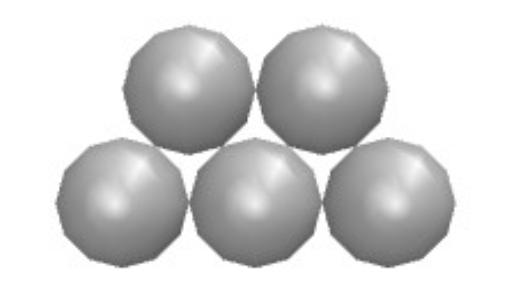
\includegraphics[width=0.25\linewidth]{Figures/fen5}
	\caption{Representation of phenanthrene with the geometry proposed by \citeonline{muller2017}. }
	\label{fig:fen5}
\end{figure}

The minimization was done using the Particle Swarm Optimization (PSO)  method \cite{pso} with the following objective function:
\begin{equation}
\min\limits_{\sigma,\epsilon,\lambda_{r}} F_{obj} = \sum_{i=1}^{N_{p}} \left[\frac{P_{v}^{SAFT}(T_{i},\sigma,\epsilon,\lambda_{r})-P_{v}^{exp}(T_{i})}{P_{v}^{exp}(T_{i})} \right]^2 .
\label{eqn:fobjm}
\end{equation}

Here, $P_{v}^{exp}$ is the experimental vapor pressure and $P_{v}^{SAFT}$ is the vapor pressure obtained with the SAFT-VR Mie EoS. We used the routine proposed by  \citeonline{smithbook} to calculate the bubble point with the EoS. The parameters ($\sigma$, $\epsilon $, and $\lambda _{r}$) from the minimization of the objective function in Eq. \eqref{eqn:fobjm} are the final force field parameters used in molecular simulations. 

The parameterization with the ring equation the \citeonline{lafitte2012} was carried out with $m_{s}=3$, so that every bead would represent one aromatic ring, as depicted in Figure \ref{fig:fen3}.

\begin{figure}[th]
	\centering
	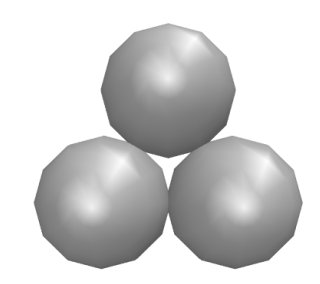
\includegraphics[width=0.15\linewidth]{Figures/fe3}
	\caption{Representation of phenanthrene with the geometry proposed by \citeonline{lafitte2012}.}
	\label{fig:fen3}
\end{figure}

The first part of the estimation followed the same procedure described above for the \citeonline{muller2017} equation. However, as explained in Section \ref{parsaft}, the \citeonline{lafitte2012} equation requires the estimation of correction factors $c_{\sigma}$ and $c_{\epsilon}$ (Eqs. \eqref{eqn:csigma} and \eqref{eqn:ceps}). We then estimated these parameters by using the PSO method with Eq. \eqref{eqn:fobjla}. In this equation, vapor pressures and saturated liquid densities from molecular simulations are required. We then decided to use the Gibbs Ensemble Monte Carlo method on the NVT ensemble, explained in Section \ref{gemc}, to obtain these equilibrium properties at eight different temperatures since this method does not use an explicit interface.

The boxes for the GEMC-NVT simulations were generated by inserting 400 molecules of phenanthrene into one liquid box and 100 molecules of phenanthrene into one vapor box using the Playmol package \cite{playmol}, which is integrated with the Packmol package \cite{packmol}. Initial densities of each box were made equal to the saturated densities found with the SAFT-VR Mie Eos, aiming at avoiding the migration of all molecules to a single phase during the simulation. The GEMC-NVT simulations were executed using the Cassandra software \cite{doi:10.1063/1.3644939},  which was developed to perform Monte Carlo simulations. The equilibration and production times lasted around  $10^{4}$ and $5 \times 10^{4}$ MC cycles, respectively. Each MC cycle corresponded to $10^3$ rotation trials, $10^3$ translation trials, $10^2$ molecule insertion trials, $10^2$ molecule deletion trials, and 10 volume exchange trials. The cut-off distance was equal to $20$ \AA  $\,$ and we did not use long-range interactions. The saturated vapor density ($\rho_{vap}$), the saturated liquid density ($\rho_{liq}$), and the vapor pressure ($P_{v}$) were sampled at each 100 MC cycles. Later on, these data were divided into five blocks for calculation of their averages and standard deviations. With the correction factors found after the estimation with the simulation data, we calculated, with Eqs. \eqref{eqn:simsigma} and \eqref{eqn:simeps}, the $\sigma$ and $\epsilon$ parameters. \citeonline{lafitte2012} proposes that these are the final parameters to be used in molecular simulations. Hence, an iterative simulation is not required and the set of optimal parameters can be obtained with one group of molecular simulations. 

\section{Solvation Free Energy Simulations}\label{solvme}

Using the parameters for phenanthrene estimated with the \citeonline{muller2017} approach and the SAFT-$\gamma$ Mie force field parameters available for other compounds, we carried out molecular dynamics simulations to estimate the solvation free energies. The chosen software package to perform the simulations was LAMMPS  \cite{lammps}. In this package, the equations of motion were integrated with the velocity-Verlet algorithm \cite{verlet} with a time step of 2 fs. As required by the coarse-grained model,  molecules with more than one bead were treated as rigid bodies. The thermostat and the barostat were the Nos\'{e}-Hoover chains as described in \citeonline{PhysRevA.31.1695}, \citeonline{doi:10.1063/1.463940}, and \citeonline{doi:10.1063/1.467468} with damping factors of 100 and 1000 time steps, respectively. For the rigid bodies in our simulations, we used the rigid-body algorithm of \citeonline{kamberaj}. Electrostatics interactions are not explicitly accounted for by the SAFT-$\gamma$ Mie force field. Hence, we did not compute Coulombic interactions. The potential cutoff was equal to 20 \AA $\,$ \cite{muller2017} with a neighbor list skin of 2 \AA. The initial configurations of the solvated systems were also generated using the Playmol package, which is integrated with the Packmol package. For the binary mixtures, one molecule of solute and a varying number of solvent molecules- 700 molecules of toluene, 700 molecules of octanol, 1024 molecules of hexane, 3000 molecules of water - were randomly added to a cubic box. Besides the systems with pure substances acting as solvents, we performed simulations to study the solvation free energy of phenanthrene in a mixture of toluene and carbon dioxide with different weight fractions ($w_{CO_{2}}$). The  system consisted of one molecule of phenanthrene for all the cases and 123 molecules of $CO_{2}$ and 618 molecules of toluene ($w_{CO_{2}} = 0.087$); 166 molecules of $CO_{2}$ and 589 molecules of toluene ($w_{CO_{2}} = 0.119$); 232 molecules of $CO_{2}$ and 545 molecules of toluene ($w_{CO_{2}} = 0.169)$; 380 molecules of $CO_{2}$ and 446 molecules of toluene ($w_{CO_{2}} = 0.289$). These substances used in our study were selected with the intention of testing the force field with standard sets used as a benchmark in solvation free energy calculations, with aromatic substances used as models to asphaltenes and with water, which probably is the most used solvent in computational studies.

All simulations were performed with the constant temperature and pressure values of 298 K and 1 bar, except the ones containing carbon dioxide. These had the temperature of 298 K and the pressure of the experimental liquid-phase equilibrium corresponding to each composition of the system $CO_{2}+$toluene \cite{co2toliq}. For all simulations, the initial box was equilibrated at the NPT ensemble for 2 ns, and the resulting configurations were used as the initial configuration of the expanded ensemble simulations. These were carried out with the LAMMPS user package for expanded ensemble simulations with the Mie potential developed by our research group, available at https://github.com/atoms-ufrj/USER-ALCHEMICAL. 

During these expanded ensemble simulations, the sampling of a new alchemical state was tried at every 10 MD steps. To define the optimal values of $\lambda$ and $\eta$ corresponding to each state, trial simulations, having around 9 ns of production time, were carried out. In the first simulation, we chose the group of $\lambda$ values arbitrarily, and we either set all $\eta 's$ to zero or assigned values previously found for similar solute-solvent pairs. The subsequent group of $\eta 's$ were estimated with the flat histogram approach (Eq. \eqref{eqn:weight}). We then performed another trial simulation with the new weights. The results of this simulation were used to optimize the group of $\lambda 's$ by minimizing the number of round trips, as described in Section \ref{ee}. The $\eta 's$ corresponding to the newest group of $\lambda 's$ were interpolated linearly from the free energy differences. With the final values of $\eta$ and $\lambda $ defined for each mixture, larger simulations with a production time of 20 ns were carried out. 

Since the employed force field considers that the beads do not have charges, there are no Coulombic interactions and the $\Delta G$ in Eq. \eqref{eq:freesolv} becomes equal to $\Delta G_{3 \rightarrow 4} $. The post-processing method used to effectively calculate free energy differences with the potential energies obtained from the expanded ensemble simulations was the Multistate Bennett Acceptance Ratio (MBAR) method, described in Section \ref{mbar}. The software alchemical-analysis \cite{klimovich} was utilized to obtain the $\Delta G_{solv}$ with MBAR and to assess the quality of the results. After the first estimations, we realized that the binary interaction parameter of Eq. \eqref{eqn:epsmix} was necessary for systems containing water. Hence, we estimated  $k_{ij}$ for these pairs and, for all the other pairs, we set  $k_{ij}$ to zero. The estimation was done by performing trial expanded ensemble simulations in three values of $k_{ij}$, as suggested by \citeonline{ervik20162}. With the $\Delta G_{solv}$ obtained with these simulations, we did a linear fit to obtain the refined value of the parameter. We used this strategy because the estimation with SAFT-VR Mie EoS gave poor results for the hydration free energies.


\chapter{Results and Discussion} % Main chapter title

\label{Chapter5} % Change X to a consecutive number; for referencing this chapter elsewhere, use \ref{ChapterX}

\section{Solvation free energies}

The first part of this work consisted of obtaining phenanthrene parameters for the SAFT-$\gamma$ Mie Force Field as described in Section \ref{parame}. This part was necessary since these parameters were not available for the ring geometry on the force field database \cite{ervik2016}. The parameters obtained and the mean percentage error (MPE) of the vapor pressure found with the SAFT-VR Mie EoS to the experimental data \cite{pvphen} were those observed in Table \ref{tbl:estimparameters}.

\begin{table*}[h]
	\centering
	\caption{Estimated SAFT-$\gamma$ Mie force field parameters for phenanthrene.}
	\label{tbl:estimparameters}
	\begin{tabular}{ccccc}
		\hline\hline
		$m_s$                & $\epsilon/\kappa_{b}$ (K) & $\sigma$ (\AA) & $\lambda_r$ & MPE(\%)   \\ \hline\hline
		3 \cite{lafitte2012} & 485.55               & 4.197              & 14.34       & 1.64|9.74 \\
		5  \cite{muller2017} & 262.74               & 4.077              & 9.55        & 0.88      \\ \hline\hline
	\end{tabular}
	
\end{table*} 

The MPE value of 1.69 for the \citeonline{lafitte2012} strategy in the Table \ref{tbl:estimparameters} is the error between the vapor pressure calculated with the equation of state and the experimental data. The other MPE value for the \citeonline{lafitte2012} strategy (9.74) is the error between the vapor pressure calculated with the equation of state and the vapor pressure obtained in the GEMC simulations. The \citeonline{lafitte2012} strategy should not need an estimation with molecular simulation data since this additional procedure is not necessary when estimating parameters for the chain equation \cite{avendano2011} or the ring equation of \citeonline{muller2017}. In addition to that, this use of molecular simulation data to acquire the parameters negates the overall idea proposed by \cite{avendano2011}. They developed this force field with the intention of obtaining the parameters in a more straightforward way than other force fields since the SAFT-$\gamma$ Mie model would not have the computational time associated with doing molecular simulations in its parameterization. Due to these specific characteristics of the model of \citeonline{lafitte2012}, we only studied the solvation free energy of phenanthrene with the set of parameters estimated with the strategy of \citeonline{muller2017}. In fact, we only followed the strategy of \citeonline{lafitte2012} because it was the only one available when we first started this research. The sets of parameters for the other compounds were retrieved from the literature \cite{lobanova2016,herdes2015,ervik2016,muller2017}, and all the utilized parameters are available in Table \ref{tbl:parameters}.

\begin{table*}[h]
	\centering
	\caption{SAFT-$\gamma$ Mie force field for each substance used in this work.}
	\label{tbl:parameters}
	\begin{tabular}{ccccc}
		\hline
		\hline
		& $m_s$ & $\epsilon/\kappa_{b}$ (K) & $\sigma$ (\AA) & $\lambda_r$ \\ \hline\hline
		Water          & 1     & 305.21               & 2.902              & 8.0         \\
		Propane        & 1     & 426.08               & 4.871              & 34.29       \\
		Carbon dioxide & 2     & 194.94               & 2.848              & 14.65       \\
		Hexane         & 2     & 376.35               & 4.508              & 19.57       \\
		Octanol        & 3     & 495.71               & 4.341              & 28.79       \\
		Toluene        & 3     & 268.24               & 3.685              & 11.80       \\
		Benzene        & 3     & 230.30               & 3.441              & 10.45       \\
		Pyrene         & 4     & 459.04               & 4.134              & 15.79       \\
		Anthracene     & 5     & 259.68               & 3.631              & 9.55        \\ 
		\hline
		\hline
	\end{tabular}
	
\end{table*}
\FloatBarrier
Our primary intention with this study is to assess the capability of the SAFT-$\gamma$ Mie force field to represent solvation free energies. Hence, we chose benchmark solutes used in the literature (benzene, propane) and polyaromatic solutes (benzene, pyrene, phenanthrene, anthracene), and, for the solvents, we picked non-polar (hexane), aromatic (toluene), and hydrogen bonding (1-octanol, water) substances. It would be interesting to do a study with a bigger database of pairs solvent-solute. However, the time required for performing each of the solvation free energy simulations, some difficulties related to the available computational structure, and the fact that a better model of aromatic compounds with this force field was only published in the middle of our study prevented us of doing a more extensive study. The solvation free energy simulations for the pairs chosen were carried with binary interaction parameters equal to zero since these parameters were not necessary according to our preliminary studies. Since the force field does not account for charges, we only calculated the Mie contribution (Eq. \eqref{eq:softcore}) to the solvation free energy. A total of 15 to 18 $\lambda 's$, depending on the solute-solvent pairs, and their respective $\eta 's$ were estimated as described in Sections \ref{ee} and \ref{solvme}. The final $\lambda$ set for all the pairs was found using the cumulative probability distribution (Eq. \eqref{eqn:cumfun}). The probability distribution for the hexane(solvent)+benzene(solute) pair can be seen in \figref{fig:optimized_cdf}. Now on we are going to use the terminology solvent+solute. The optimized values of $\lambda$ and $\eta$ for this pair and all the other pairs are available in Tables \ref{tbl:lambdahex} to \ref{tbl:lambdaco2}. Observing the coupling parameters found for all the pairs, we can see that they are concentrated on the region with a steeper slope as it is expected in this method.

\begin{figure}[h]
	\centering
	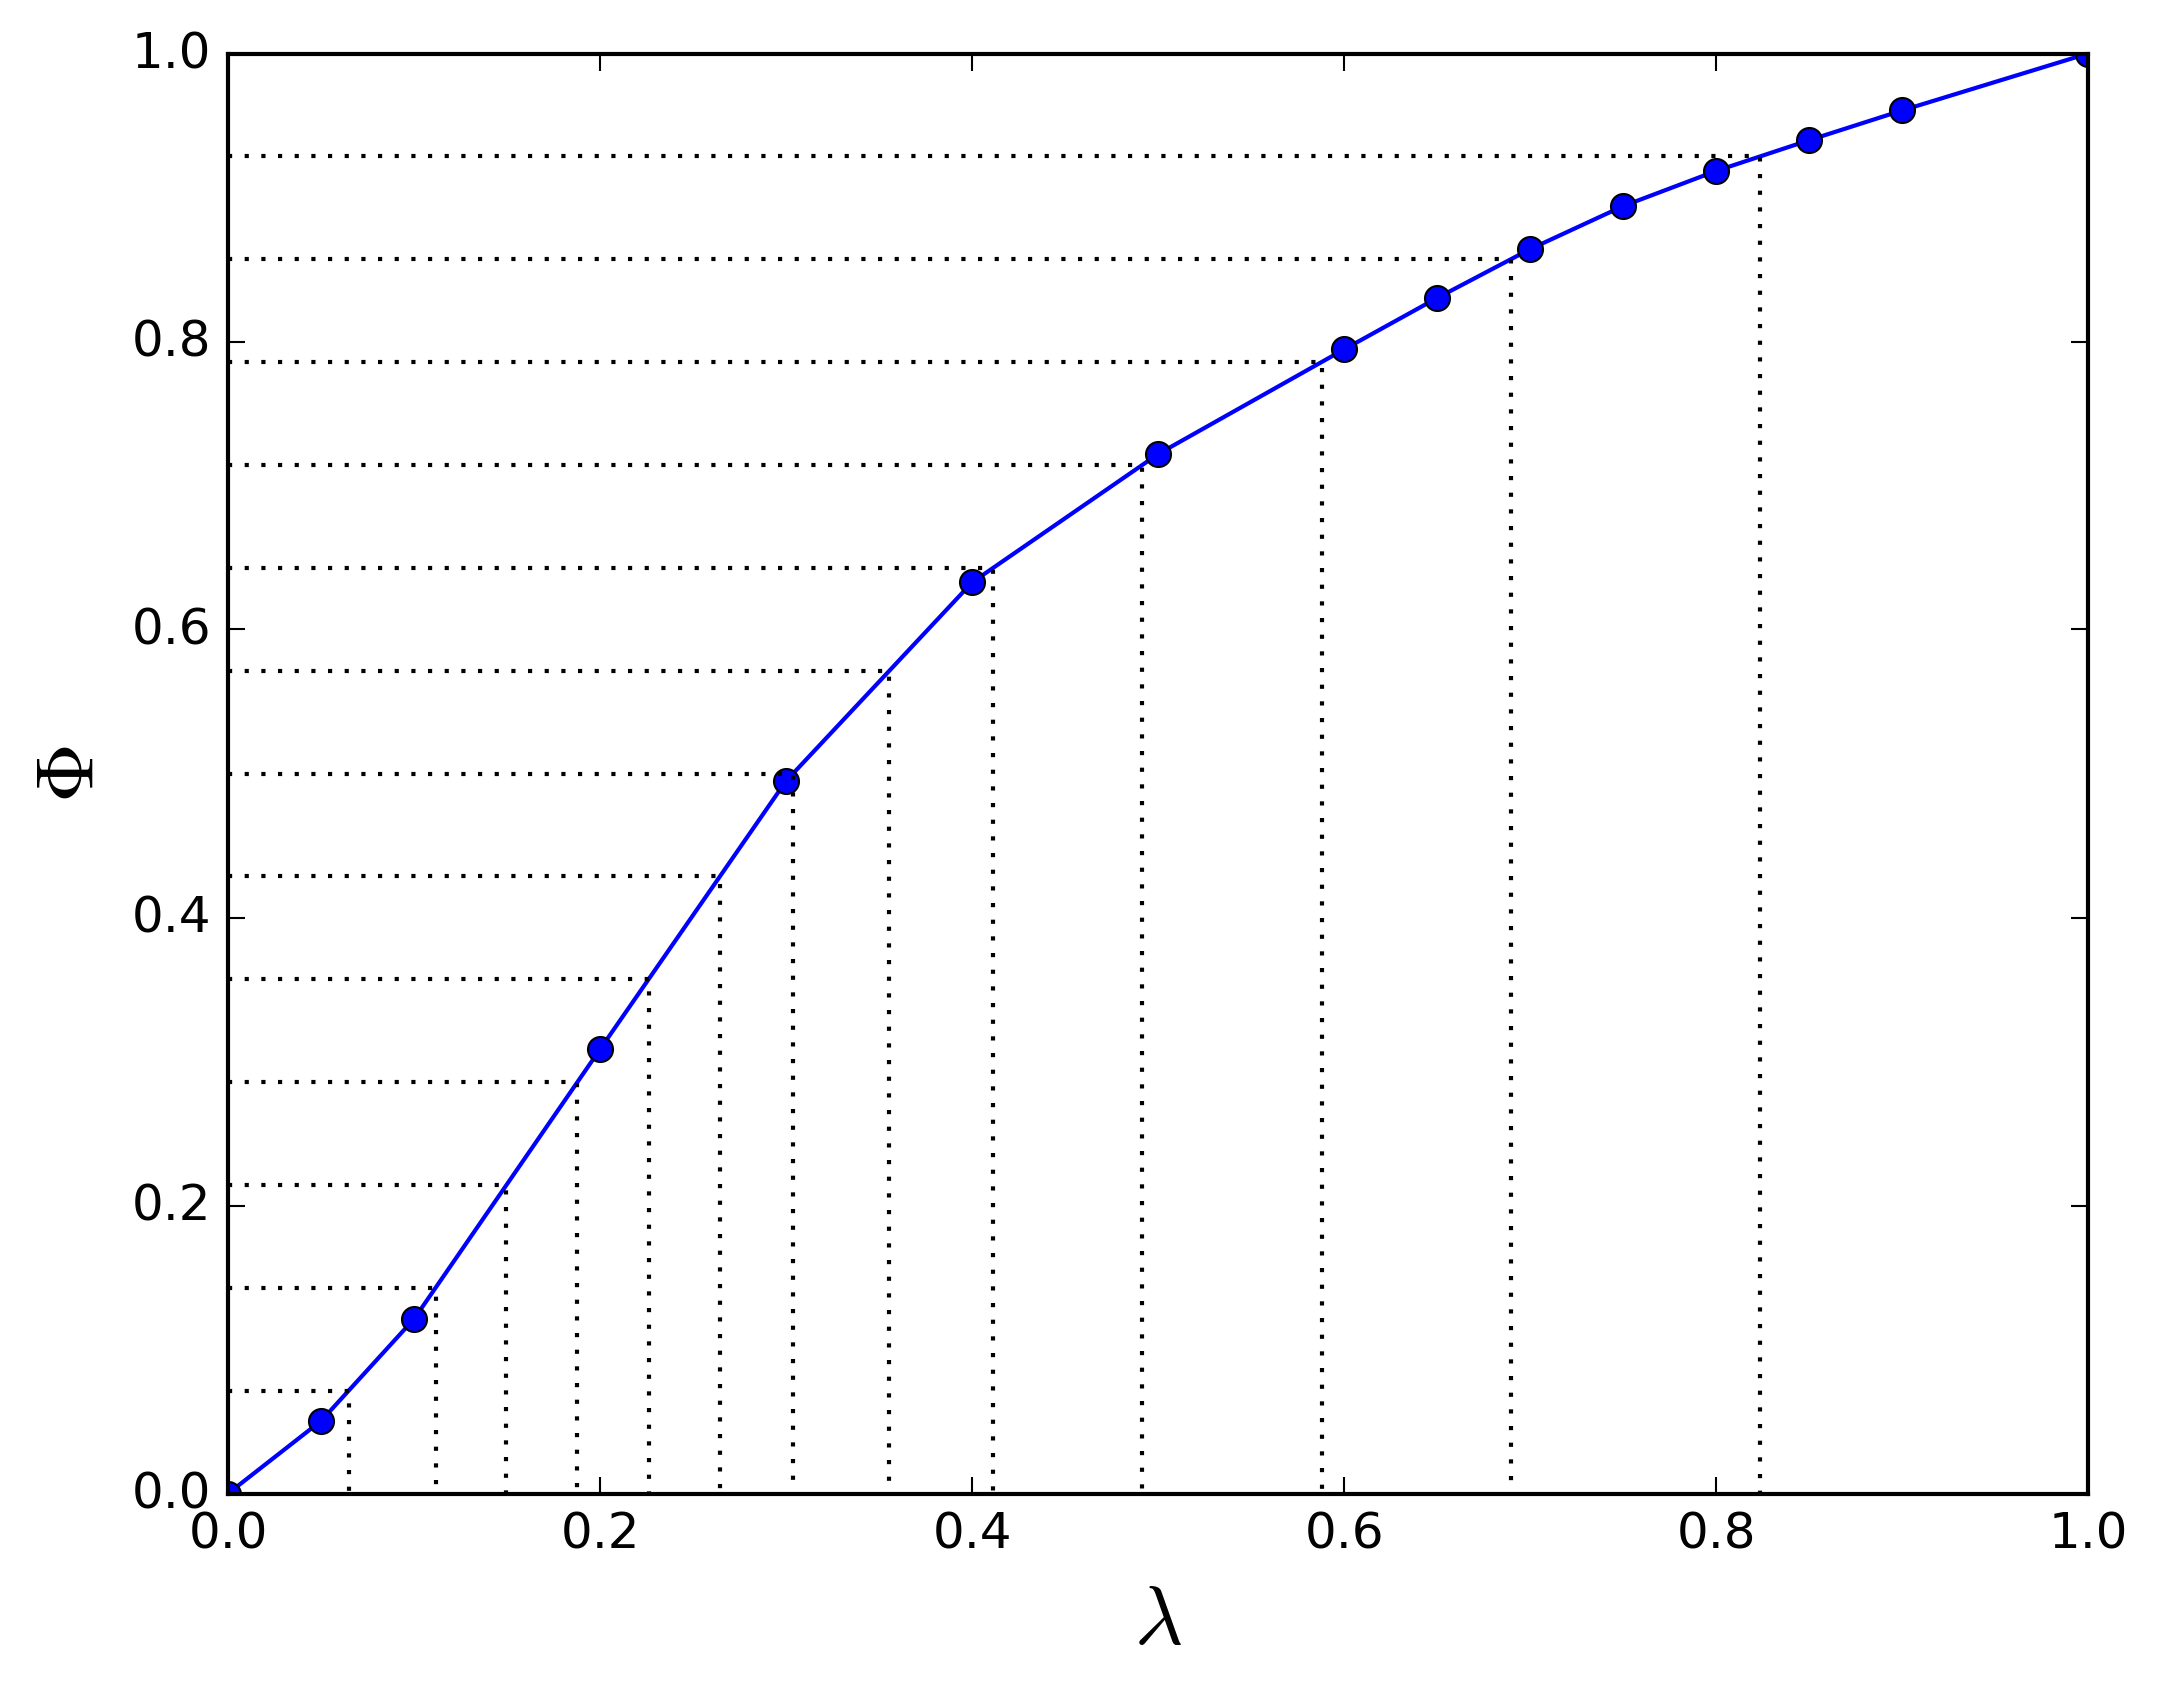
\includegraphics[width=0.8\linewidth]{Figures/optimized_cdf}
	\caption{Cumulative probability used to obtain the optimized values of $\lambda 's$ for the pair hexane+benzene.}
	\label{fig:optimized_cdf}
\end{figure}
\begin{table*}[h]
	\centering
	\caption{Optimized values of $\lambda $ and $\eta $ for the hexane+solute pairs.}
	\label{tbl:lambdahex}
	\begin{tabular}{cccccc}
		\hline\hline
		\multicolumn{2}{c}{benzene}&\multicolumn{2}{c}{pyrene}& \multicolumn{2}{c}{phenanthrene}\\
		\hline\hline
		$\lambda$ & $\eta$& $\lambda$ & $\eta$  & $\lambda$ & $\eta$   \\ 
		\hline\hline
		0.000     &0.000      & 0.000    &    0.000    &    0.000    &    0.000    \\
		0.065     &0.708  & 0.076    &    4.234    &    0.090    &    1.981    \\
		0.112     &1.385  & 0.107    &    5.620    &    0.132    &    3.461    \\
		0.15      &1.892  & 0.132    &    6.499    &    0.161    &    4.494    \\
		0.188     &2.399  & 0.152    &    6.690    &    0.185    &    5.185    \\
		0.226     &2.519  & 0.170    &    6.643    &    0.205    &    5.552    \\
		0.264     &2.457  & 0.189    &    6.461    &    0.224    &    5.725    \\
		0.304     &2.367  & 0.213    &    6.091    &    0.244    &    5.722    \\
		0.356     &1.921  & 0.242    &    5.566    &    0.268    &    5.523    \\
		0.411     &1.411  & 0.280    &    4.729    &    0.305    &    4.975    \\
		0.492     &0.524  & 0.355    &    2.853    &    0.372    &    3.576    \\
		0.588     &-0.663 & 0.483    &    -0.778    &    0.500    &    0.297    \\
		0.69      &-2.016 & 0.678    &    -6.947    &    0.560    &    -1.390    \\
		0.824     &-3.922 & 0.788    &    -10.631    &    0.722    &    -6.309    \\
		1.000         &-6.583  &1.000      &    -18.141    &    1.000    &    -15.448    \\
		\hline\hline   
	\end{tabular}
\end{table*}
\begin{table*}[h]
	\centering
	\caption{Optimized values of $\lambda $ and $\eta$ for the 1-octanol+solute pairs.}
	\begin{tabular}{cccccc}
		\hline\hline
		\multicolumn{2}{c}{propane}& \multicolumn{2}{c}{anthracene}& \multicolumn{2}{c}{phenanthrene}\\
		\hline\hline
		$\lambda$ & $\eta$ & $\lambda$ & $\eta$  & $\lambda$ & $\eta$   \\ 
		\hline\hline
		0.000    &    0.000    &    0.000    &    0.000    &    0.000    &    0.000    \\
		0.027    &    3.126    &    0.078    &    3.932    &    0.049    &    2.578    \\
		0.050    &    5.109    &    0.111    &    6.178    &    0.091    &    5.663    \\
		0.073    &    6.093    &    0.130    &    7.426    &    0.125    &    8.575    \\
		0.095    &    6.570    &    0.143    &    8.201    &    0.144    &    10.069    \\
		0.117    &    6.826    &    0.154    &    8.717    &    0.157    &    10.978    \\
		0.142    &    6.956    &    0.164    &    9.085    &    0.169    &    11.599    \\
		0.174    &    6.969    &    0.174    &    9.357    &    0.180    &    12.040    \\
		0.215    &    6.847    &    0.184    &    9.556    &    0.192    &    12.340    \\
		0.269    &    6.554    &    0.197    &    9.676    &    0.206    &    12.499    \\
		0.337    &    6.050    &    0.214    &    9.681    &    0.225    &    12.478    \\
		0.427    &    5.228    &    0.238    &    9.490    &    0.253    &    12.161    \\
		0.545    &    3.955    &    0.274    &    8.958    &    0.298    &    11.280    \\
		0.720    &    1.843    &    0.326    &    7.906    &    0.371    &    9.406    \\
		1.000    &    -1.903    &    0.399    &    6.088    &    0.484    &    5.891    \\
		&        &    0.515    &    2.777    &    0.664    &    -0.516    \\
		&        &    0.695    &    -2.960    &    0.802    &    -5.908    \\
		&        &    1.000    &    -13.768    &    1.000    &    -14.073    \\
		\hline\hline
	\end{tabular}
\end{table*}
\begin{table*}[h]
	\centering
	\caption{Optimized values of $\lambda $ and $\eta$ for the toluene+solute pairs.}
	\begin{tabular}{cccccc}
		\hline\hline
		\multicolumn{2}{c}{pyrene}& \multicolumn{2}{c}{anthracene}& \multicolumn{2}{c}{phenanthrene}\\
		\hline\hline
		$\lambda$ & $\eta$ & $\lambda$ & $\eta$  & $\lambda$ & $\eta$   \\ 
		\hline\hline
		0.000    &    0.000    &    0.000    &    0.000    &    0.000    &    0.000    \\
		0.090    &    2.563    &    0.119    &    0.218    &    0.136    &    0.726    \\
		0.130    &    4.338    &    0.174    &    1.210    &    0.191    &    2.307    \\
		0.154    &    5.439    &    0.209    &    2.052    &    0.223    &    3.430    \\
		0.172    &    6.181    &    0.236    &    2.664    &    0.246    &    4.233    \\
		0.188    &    6.670    &    0.261    &    3.122    &    0.264    &    4.780    \\
		0.204    &    6.986    &    0.283    &    3.378    &    0.281    &    5.149    \\
		0.222    &    7.121    &    0.306    &    3.449    &    0.299    &    5.354    \\
		0.244    &    7.025    &    0.332    &    3.311    &    0.318    &    5.389    \\
		0.278    &    6.520    &    0.360    &    2.936    &    0.340    &    5.222    \\
		0.340    &    5.010    &    0.399    &    2.209    &    0.372    &    4.717    \\
		0.462    &    1.247    &    0.466    &    0.567    &    0.425    &    3.440    \\
		0.616    &    -4.283    &    0.564    &    -2.211    &    0.524    &    0.444    \\
		0.788    &    -11.032    &    0.715    &    -6.983    &    0.701    &    -5.814    \\
		1.000    &    -19.814    &    1.000    &    -16.923    &    1.000    &    -17.803    \\        
		\hline\hline
	\end{tabular}
\end{table*}
\begin{table*}[h]
	\centering
	\caption{Optimized values of $\lambda $ and $\eta $ for the phenanthrene+$CO_{2}$+ toluene mixture with different values of $w_{CO_{2}}$.}
	\label{tbl:lambdaco2}
	\begin{tabular}{cccccccc}
		\hline\hline
		\multicolumn{2}{c}{$w_{CO_{2}}=0.087$}& \multicolumn{2}{c}{$w_{CO_{2}}=0.119$}& \multicolumn{2}{c}{$w_{CO_{2}}=0.169$}& \multicolumn{2}{c}{$w_{CO_{2}}=0.289$}\\
		\hline\hline
		$\lambda$ & $\eta$ & $\lambda$ & $\eta$  & $\lambda$ & $\eta$  & $\lambda$ & $\eta$ \\ 
		\hline\hline
		0.000    &    0.000    &    0.000    &    0.000    &    0.000    &    0.000    &    0.000    &    0.000    \\
		0.128    &    0.604    &    0.128    &    0.732    &    0.064    &    0.883    &    0.066    &    0.806    \\
		0.184    &    2.067    &    0.186    &    2.223    &    0.108    &    0.764    &    0.111    &    0.760    \\
		0.217    &    3.164    &    0.219    &    3.319    &    0.175    &    1.969    &    0.172    &    1.983    \\
		0.240    &    3.940    &    0.244    &    4.098    &    0.214    &    3.156    &    0.204    &    2.967    \\
		0.260    &    4.472    &    0.267    &    4.704    &    0.240    &    3.974    &    0.227    &    3.627    \\
		0.277    &    4.823    &    0.289    &    5.031    &    0.258    &    4.457    &    0.245    &    4.082    \\
		0.295    &    5.035    &    0.313    &    5.084    &    0.273    &    4.750    &    0.262    &    4.395    \\
		0.318    &    5.059    &    0.339    &    4.950    &    0.287    &    4.921    &    0.279    &    4.583    \\
		0.347    &    4.762    &    0.373    &    4.371    &    0.305    &    4.962    &    0.299    &    4.621    \\
		0.397    &    3.753    &    0.425    &    3.055    &    0.326    &    4.885    &    0.325    &    4.423    \\
		0.491    &    1.031    &    0.488    &    1.196    &    0.361    &    4.401    &    0.365    &    3.739    \\
		0.670    &    -5.148    &    0.525    &    -0.027    &    0.419    &    2.990    &    0.428    &    2.198    \\
		0.791    &    -9.713    &    0.730    &    -7.185    &    0.527    &    -0.299    &    0.530    &    -0.842    \\
		1.000    &    -18.098    &    1.000    &    -17.769    &    0.697    &    -6.180    &    0.701    &    -6.763    \\
		&        &        &        &    1.000    &    -17.998    &    1.000    &    -18.163    \\
		\hline\hline
	\end{tabular}
\end{table*}
\FloatBarrier
It is also essential to analyze the reliability of solvation free energy estimations through the overlapping of the intermediate states. Insufficient overlap among states when using FEP based methods such as MBAR may result in the underestimation of variance and, consequently, in substantially incorrect solvation free energies \cite{klimovich}. The overlap matrix for the solvation free energy of benzene in hexane is presented in \figref{fig:hexove} and the matrices for the other pairs are available in Appendix \ref{overlapmatrix}. Each element $ij$ of these matrices is the average probability of observing a configuration sampled from state i in state j. As an example, the average probability of finding a configuration sampled from state 3 in state 4 is 0.11 in \figref{fig:hexove}. According to \citeonline{klimovich}, a tridiagonal overlap matrix is an indication of reliable free energy estimates, as long as the resulting error is sufficiently low. They define a tridiagonal matrix as one matrix with elements appreciable different from zero (the values should be as low as 0.03) in the main diagonal and the first diagonals above and below the main one. This requirement was met for all the pairs in our study. Some of the overlap matrices, including the one in Figure \ref{fig:hexove}, had more than three diagonals, and, consequently, an apparent unnecessary number of intermediate states. However, this number of intermediate states were indispensable in our study because the error estimate of the solvation free energies significantly increased when we removed some of the intermediate states. Hence, we maintained these intermediate states in order to obtain low error values. After this analysis, we present in Table \ref{tbl:solv1} the results for solvation free energy calculations and the absolute deviations from experimental data \cite{doi:10.1021/ci034120c}.  

\begin{figure*}[h]
	\centering
	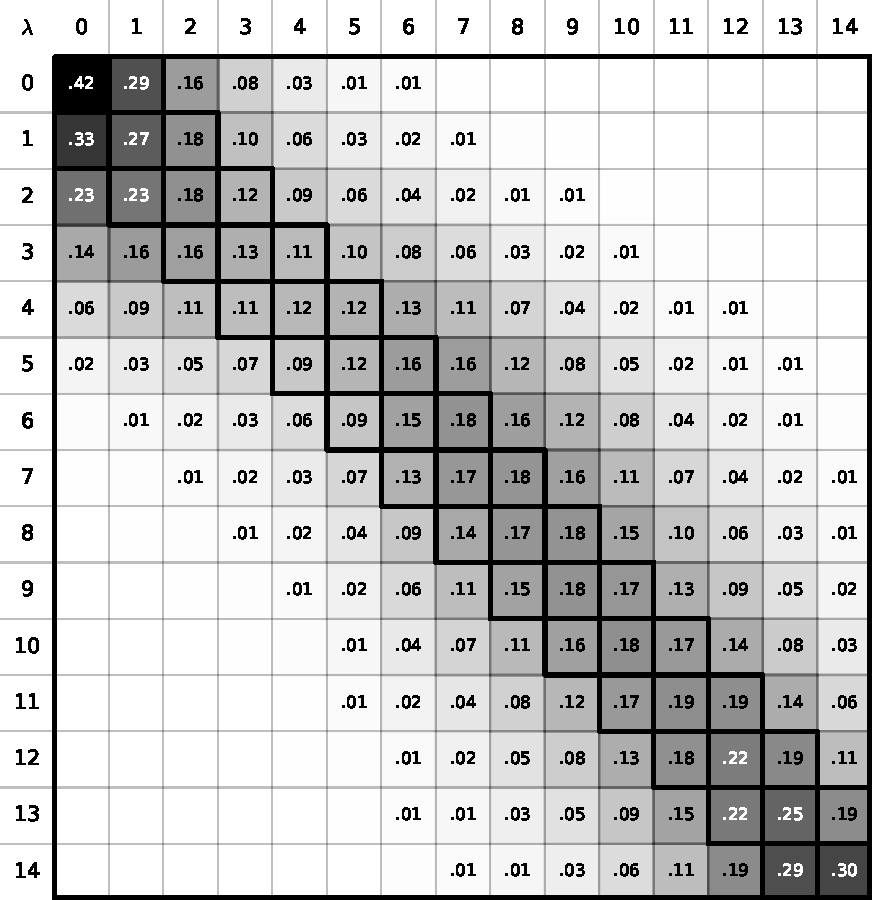
\includegraphics[width=0.7\textwidth]{Figures/ohex_benz}
	\caption{Overlap matrix for hexane+benzene.}
	\label{fig:hexove}
\end{figure*}
\FloatBarrier
\begin{table*}[h]
	\centering
	\caption{Calculated and experimental values for the solvation free energies (kcal/mol) of solutes in non-aqueous solvents.}
	\label{tbl:solv1}
	\begin{tabular}{cccccc}
		\hline\hline
		Solute       & Solvent   & $\Delta G_{solv}^{exp}$ & $\Delta G_{solv}^{Mie}$ & Absolute  &  \\
		&           &                         &                         & Deviation &  \\ \hline\hline
		benzene      & hexane    & -3.96                   & -3.76  $\,$ $\pm$ 0.01       & 0.20      &  \\
		pyrene       & hexane    & -11.53                  & -10.82 $\pm$ 0.02       & 0.71      &  \\
		phenanthrene & hexane    & -10.01                  & -9.16  $\,$ $\pm$ 0.01       & 0.85      &  \\
		propane      & 1-octanol & -1.32                   & -1.36  $\,$ $\pm$ 0.03       & 0.04      &  \\
		anthracene   & 1-octanol & -11.72                  & -8.12   $\,$ $\pm$ 0.03       & 3.61      &  \\
		phenanthrene & 1-octanol & -10.22                  & -8.34  $\,$ $\pm$ 0.03       & 1.47      &  \\
		pyrene       & toluene   & -12.86                  & -11.74 $\pm$ 0.01       & 1.11      &  \\
		anthracene   & toluene   & -11.31                  & -9.90 $\,$ $\pm$ 0.01        & 1.41      &  \\ \hline\hline
		&
	\end{tabular}
\end{table*}


The numerical values for solvation free energies in hexane had overall smaller absolute deviations from experimental data than the deviations in the other solvents. Additionally, this force field presented better results for the pair hexane+benzene than the TraPPE force field (- 4.35  $\pm$ 0.05 kcal/mol) \cite{garrido2011} and the ELBA coarse-grained force field  (-2.92 $\pm$ 0.01 kcal/mol) \cite{doi:10.1021/acs.jctc.5b00963}. TraPPE is a force field parametrized with fluid-phase equilibria data that uses the Lennard-Jones potential to describe the non-bonded interactions. In the cited paper, they used the united-atom description of the TraPPE force field for the alkyl group, the all-atom description for the polar groups and the explicit-hydrogen approach for the aromatic groups. In the explicit-hydrogen approach, the interaction sites for all hydrogen atoms, some lone pair electrons, and bond centers are accounted for \cite{doi:10.1021/jp073586l}. In turn, the ELBA force field is a coarse-grained model that comprises six independent parameters. This force field models three carbons as one Lennard-Jones site and one water molecule as a single Lennard Jones site with a point dipole. We also present the solvation free energies correspondent to each alchemical state ($\lambda$) for all the pairs studied here in Figures \ref{fig:hex} to \ref{fig:tol}. Specifically observing the solvation free energy in hexane (Figure \ref{fig:hex}), we can see the effect of the molecule's size on the entropic region of the free energy curve. This region is correspondent to the first values of $\lambda$ where space in the solvent is being 'opened' for the insertion of the solute.

We expected that a force field based on an EoS that does not explicitly account for hydrogen bond would not perform well for 1-octanol in mixtures since the parameterization of this molecule did not explicitly account for the interactions of association. All the beads representing 1-octanol have the same intermolecular parameter, and there is no distinction between the polar and apolar groups. Despite this, the solvation free energies of propane and phenanthrene in 1-octanol lied in the desired deviation range of 1-2 kcal/mol \cite{doimobley}. For propane, the observed deviation in solvation free energies was much smaller when compared to the other solutes, which can be attributed to the non polarity of propane and its smoother free energy curve, presented in Figure \ref{fig:oct}. Such solvation free energy of propane in 1-octanol also had a smaller deviation than the prediction of the ELBA force field (-0.92 $\pm$ 0.01) \cite{doi:10.1021/acs.jctc.5b00963}. The absolute deviation of the solvation free energy computed for anthracene in 1-octanol is much higher than the one calculated for phenanthrene in 1-octanol. The anthracene and phenanthrene molecules have the same geometry (Figure \ref{fig:fen5}) in the SAFT-$\gamma$ Mie model, although anthracene is a linear molecule and phenanthrene is not, and also similar physical properties. Hence, this high deviation of the solvation free energy of anthracene in 1-octanol may indicate a problem in the geometry chosen for anthracene in the SAFT-$\gamma$ Mie force field and the importance of the geometry in modeling the molecules with this force field.      

\begin{figure}[H]
	\centering
	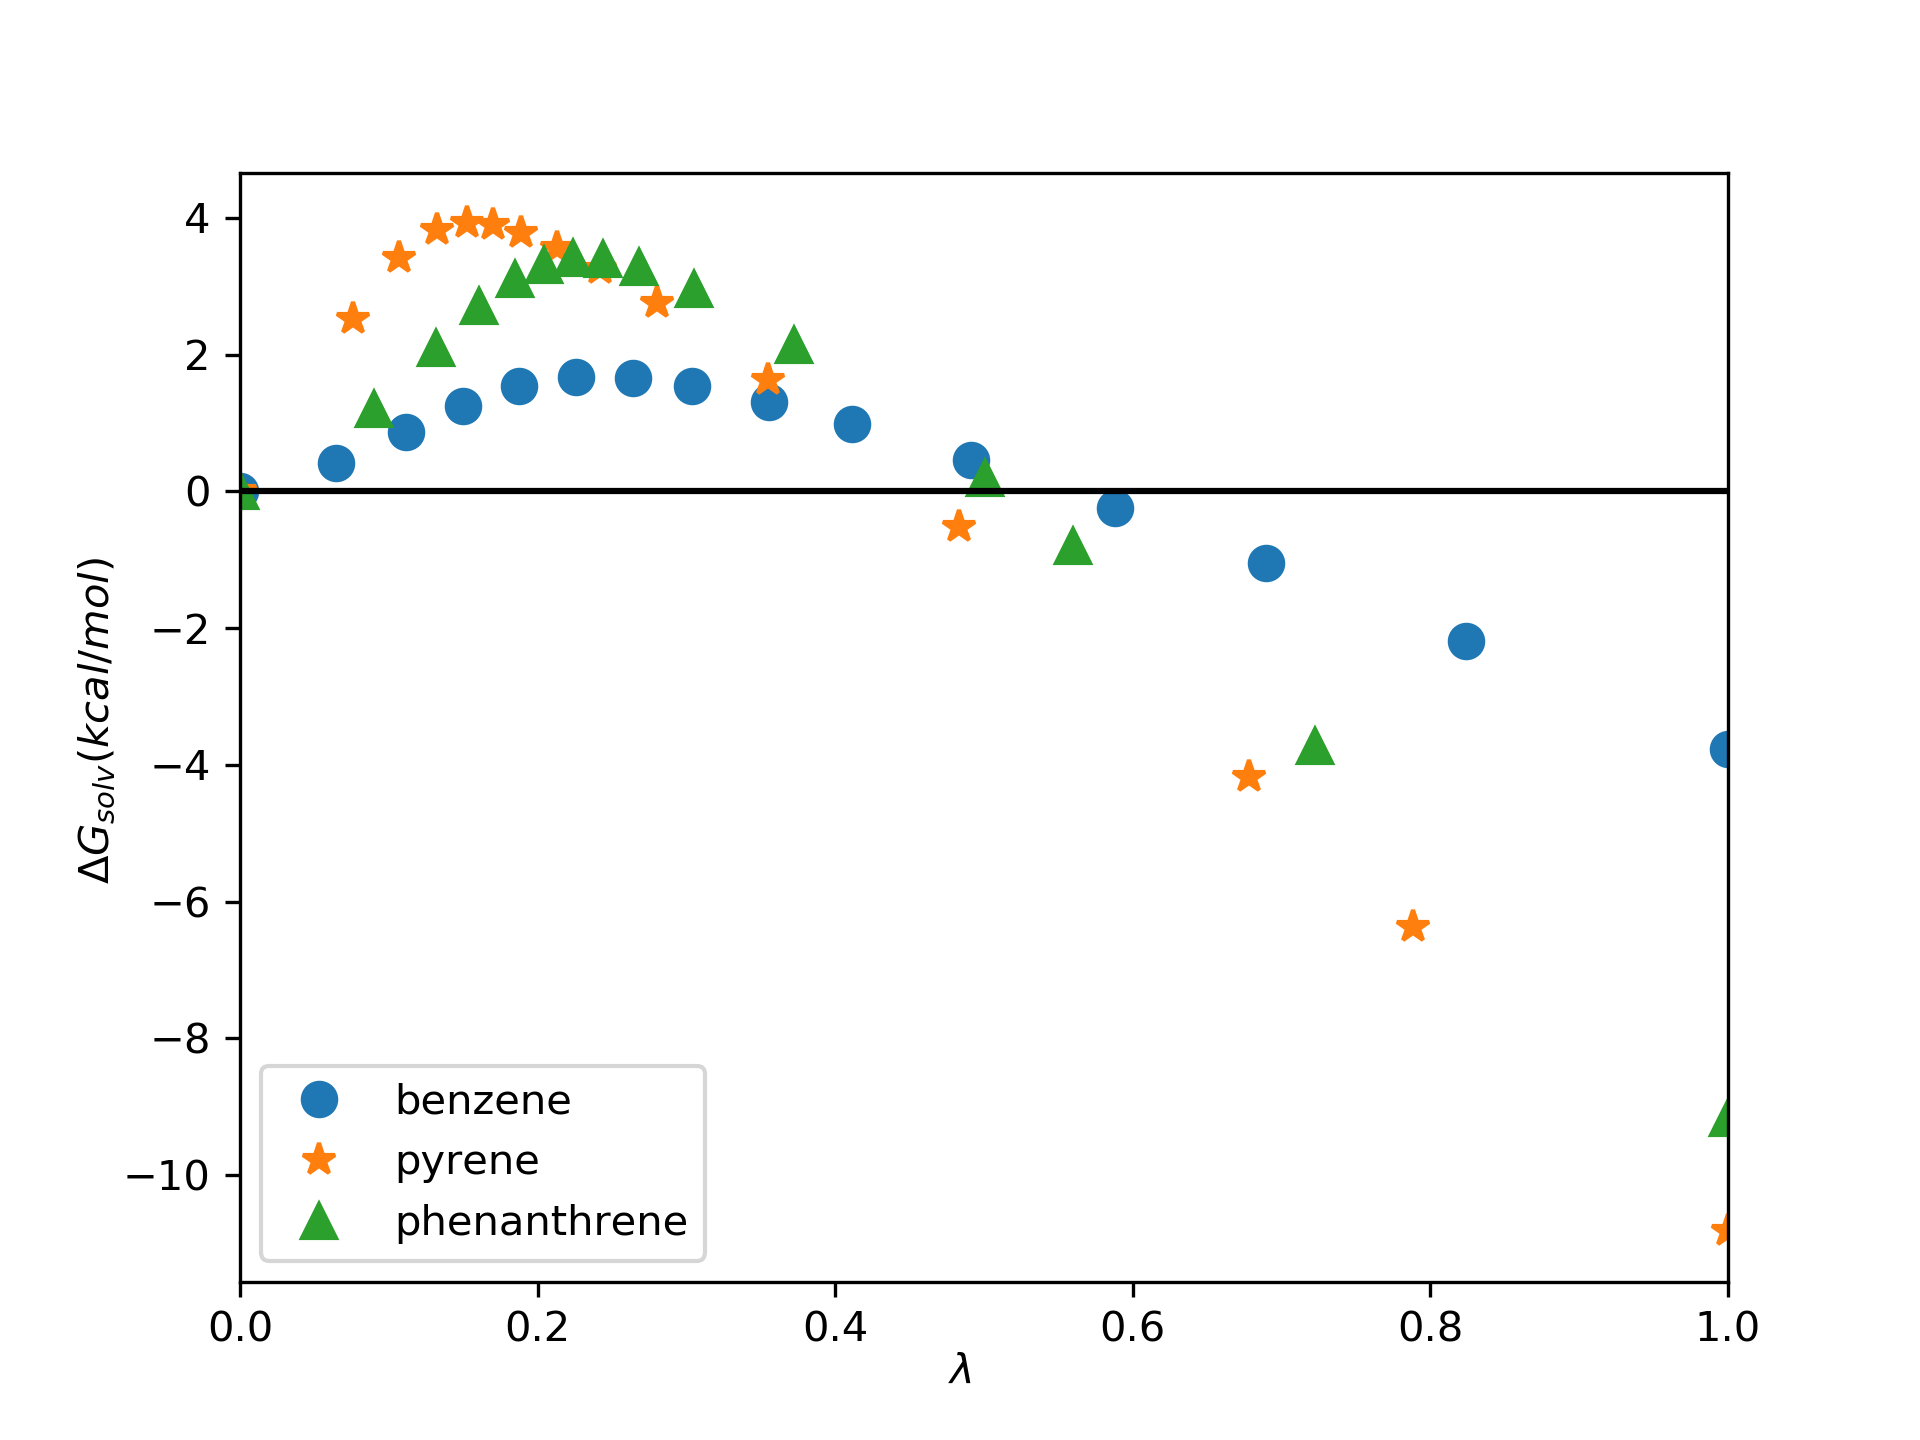
\includegraphics[width=0.8\textwidth]{Figures/hex}
	\caption{Representation of solvation free energies of different solutes in hexane correspondent to each alchemical state.}
	\label{fig:hex}
\end{figure}

\begin{figure}[H]
	\centering
	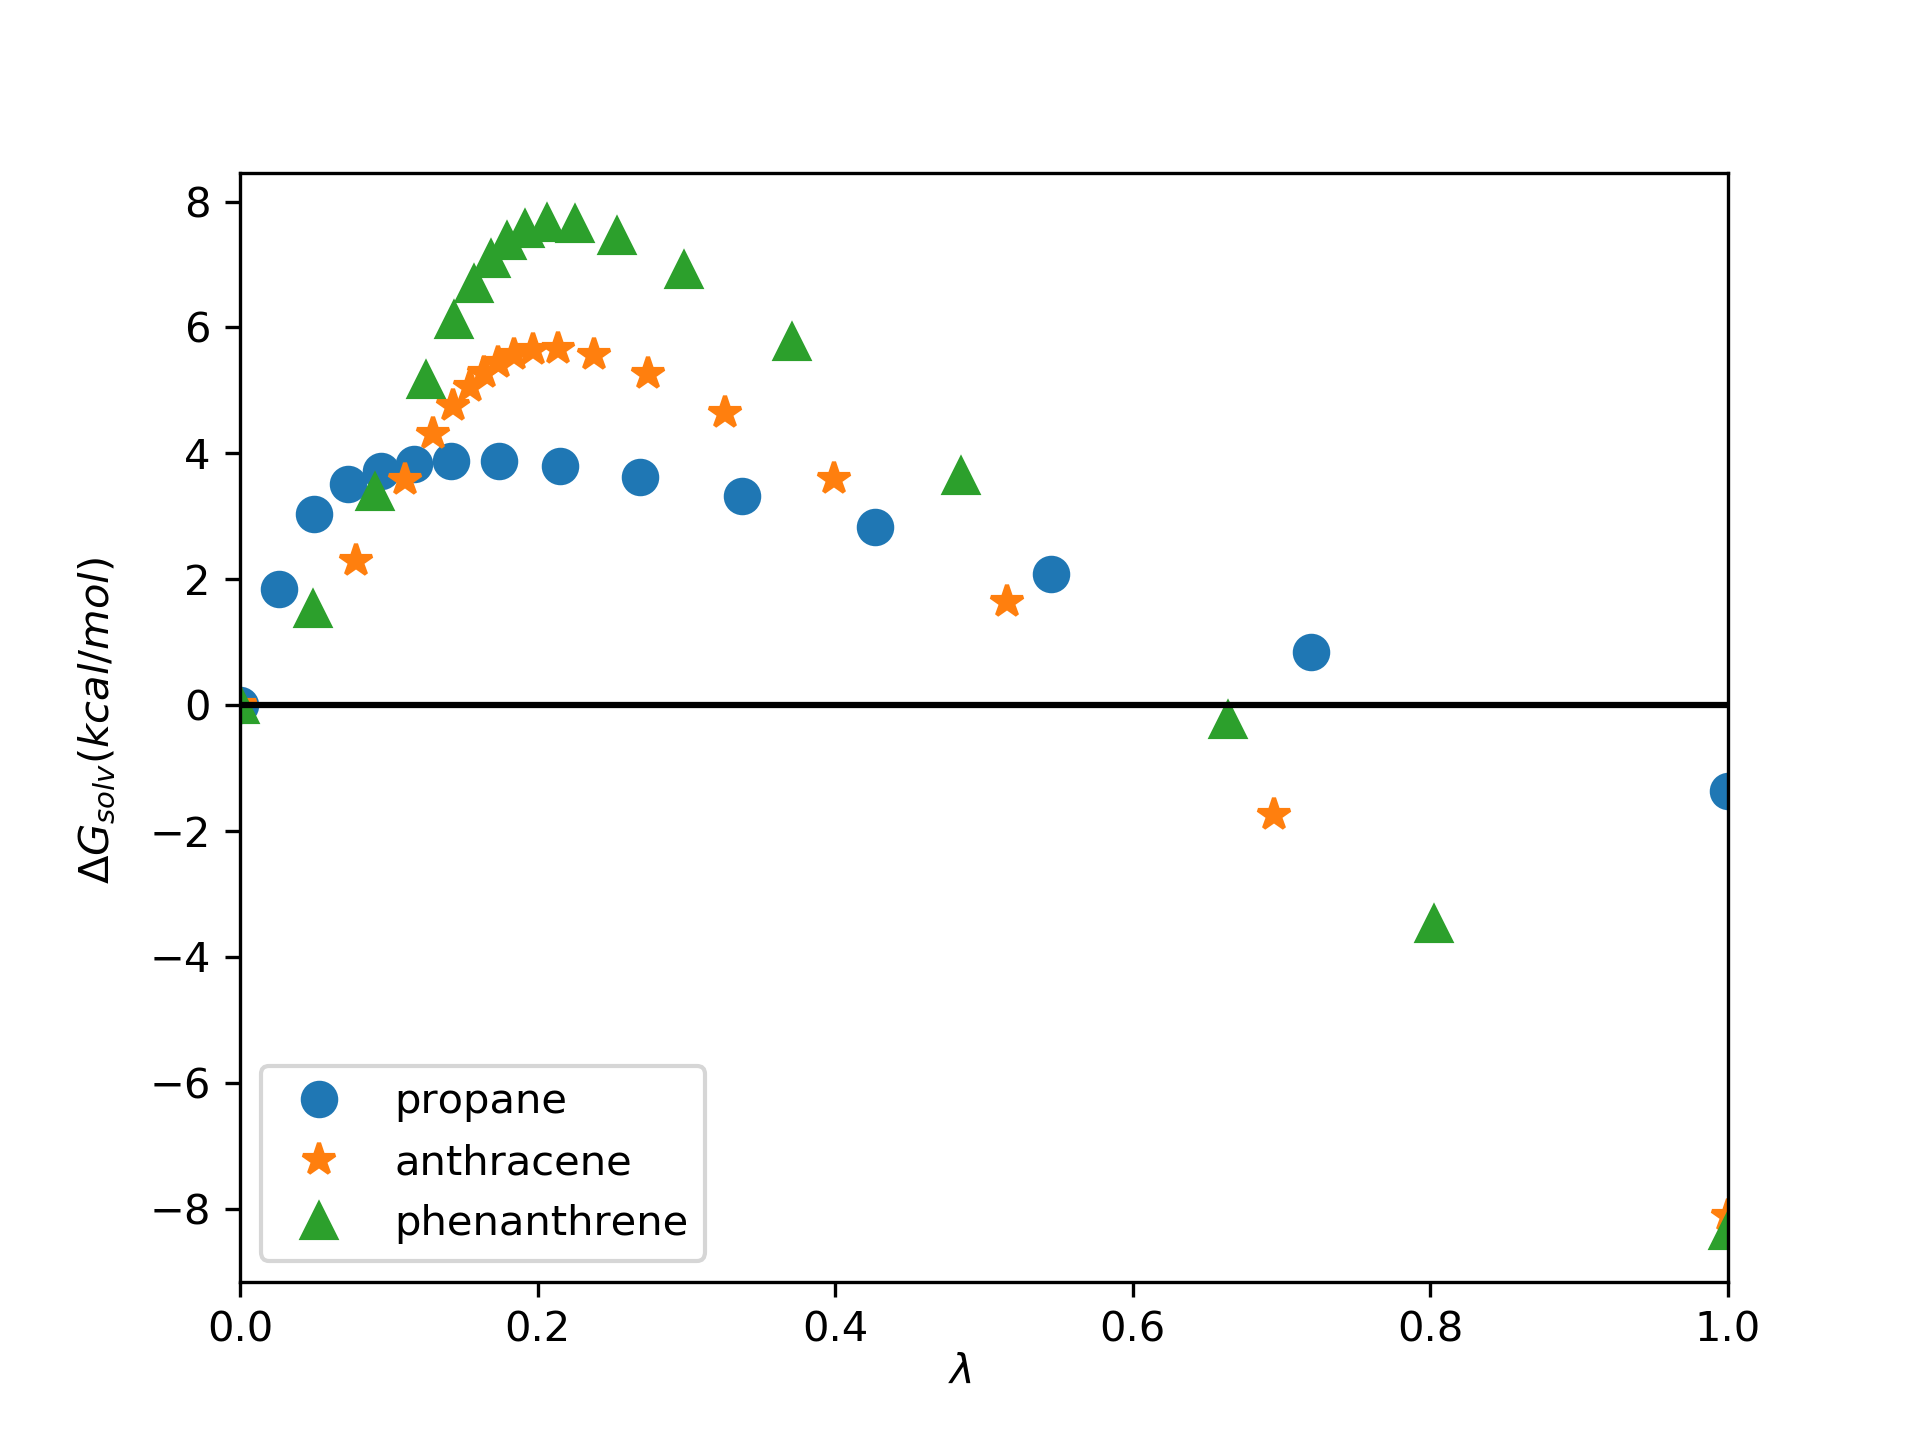
\includegraphics[width=0.8\textwidth]{Figures/oct}
	\caption{Representation of solvation free energies of different solutes in 1-octanol correspondent to each alchemical state.}
	\label{fig:oct}
\end{figure}

\begin{figure}[H]
	\centering
	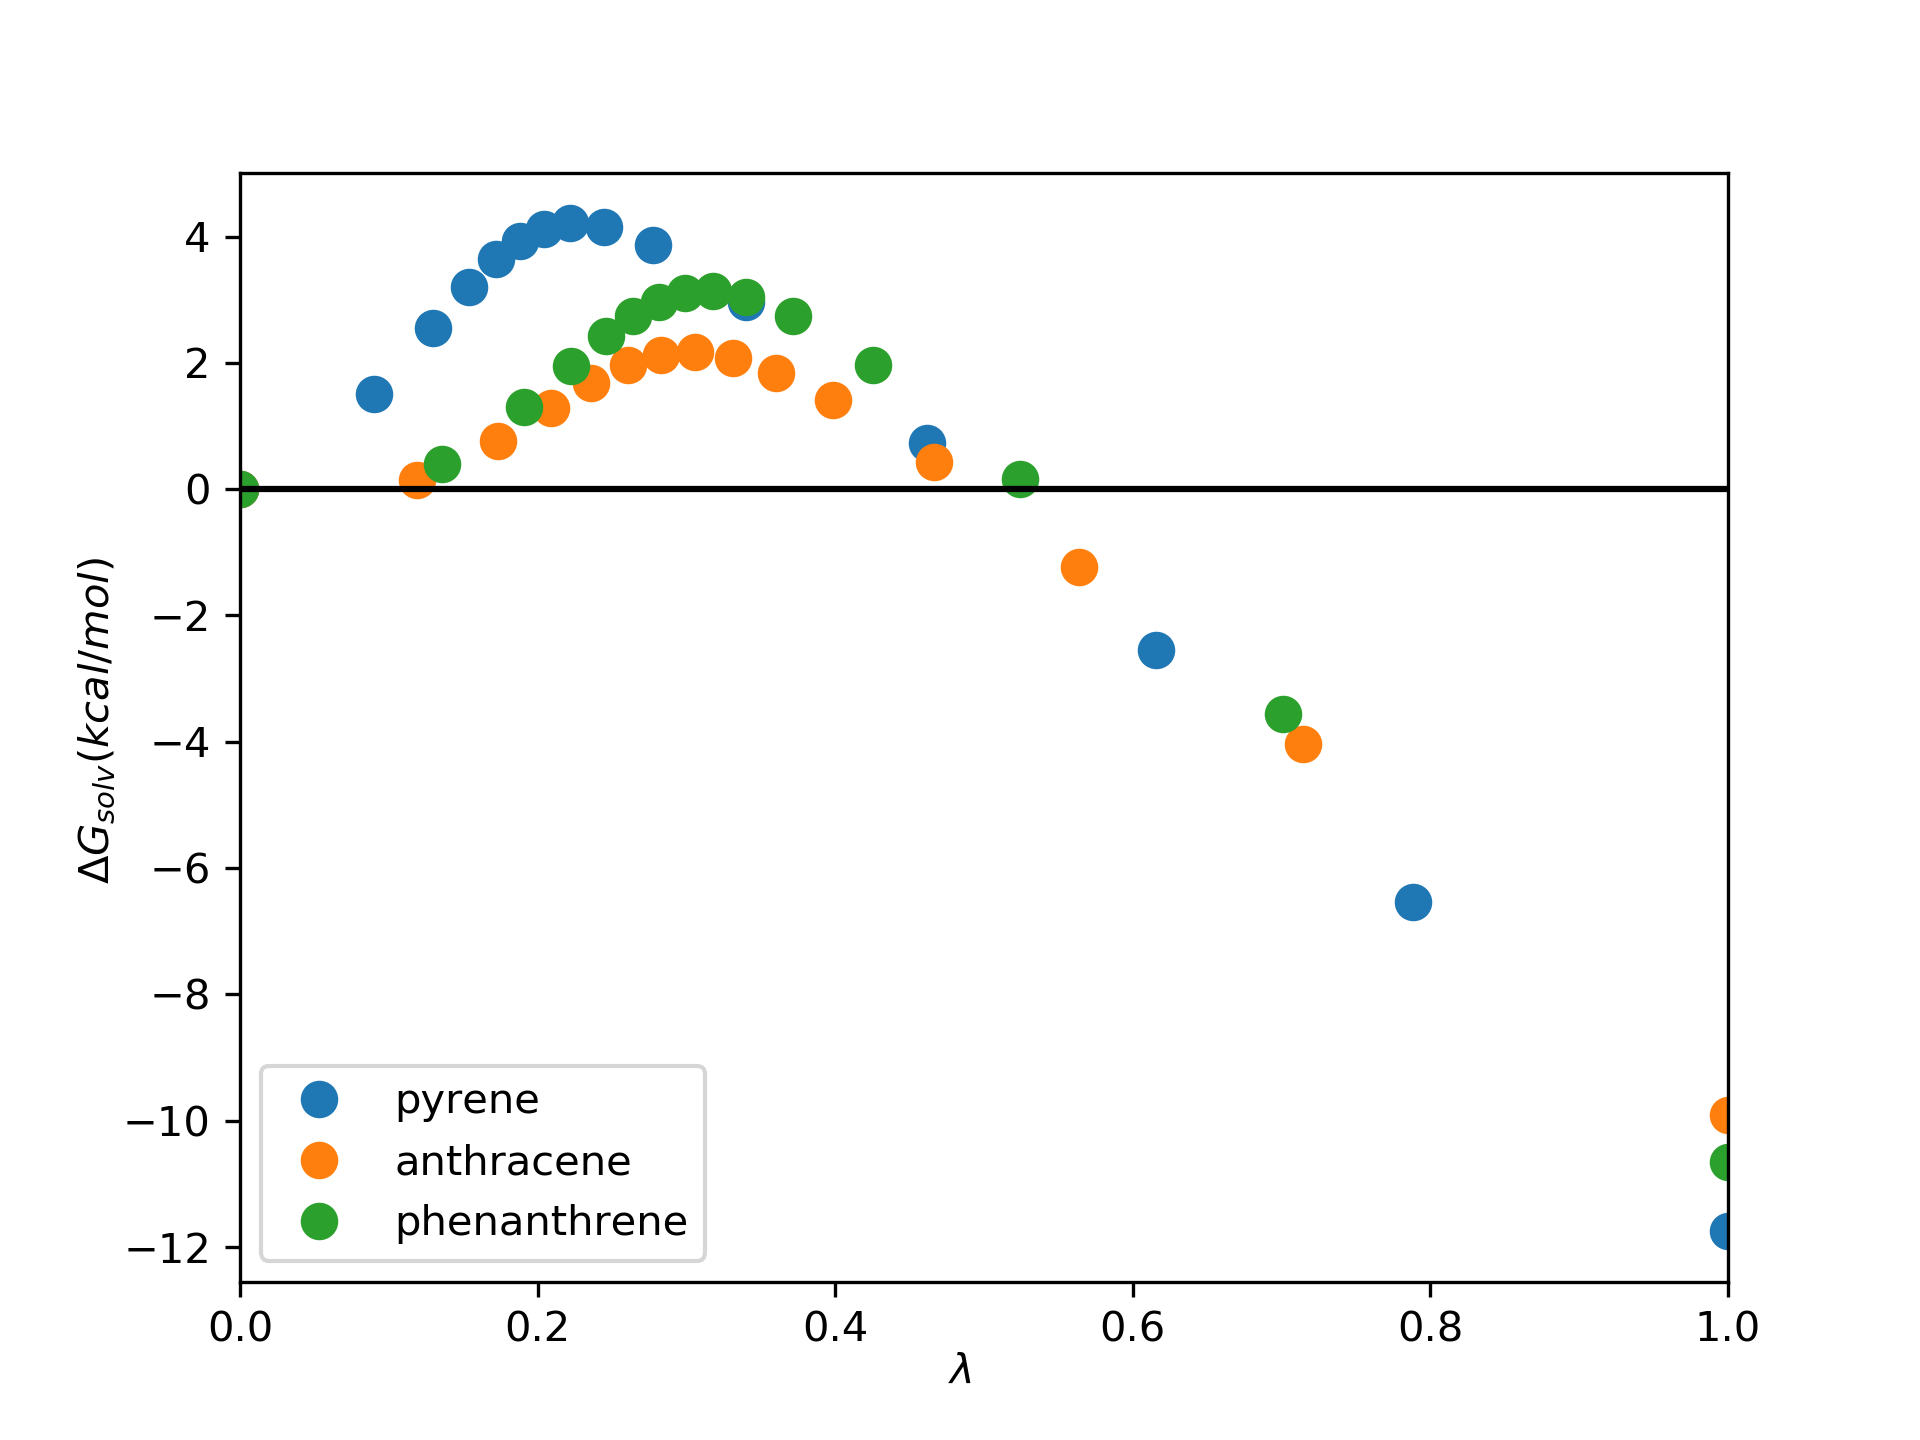
\includegraphics[width=0.8\linewidth]{Figures/tol}
	\caption{Representation of solvation free energies of different solutes in toluene correspondent to each alchemical state. }
	\label{fig:tol}
\end{figure}

The results also indicate a reasonable capability of the force field for predicting the solvation free energies of polyaromatic solutes in aromatic solvents. The influence of the molecular geometry on the solvation free energy curves was the same as the one observed for other solvents, as can be seen in Figure \ref{fig:tol}.  We also calculated the $\Delta G_{solv}$ for phenanthrene in pure toluene and in toluene+$CO_{2}$ mixtures. To the best of our knowledge, there are no available experimental data for these solvation free energies, but the previous results for phenanthrene in other solvents showed that the force field is adequate to describe the solvation phenomenon of phenanthrene in a pure aromatic solvent. Hence, we decided to carry out a qualitative study of the influence of $CO_{2}$ in the solvation free energies of phenanthrene in toluene in order to evaluate the description of this system with the SAFT-$\gamma$ Mie force field. The results for these sets are exposed in Table \ref{tbl:solvco2}.  

\FloatBarrier
\begin{table}[H]
	\centering
	\caption{Calculated values for the solvation free energies (kcal/mol) of phenanthrene in toluene+$CO_{2}$.}
	\label{tbl:solvco2}
	\begin{tabular}{cc}
		\hline
		\hline
		$w_{CO_{2}}$ & $\Delta G_{solv}^{Mie}$ \\
		\hline\hline
		0.0    & -10.65 $\pm$ 0.02   \\
		0.087  & -10.73 $\pm$ 0.02   \\
		0.119  & -10.78 $\pm$ 0.02   \\
		0.169  & -10.71 $\pm$ 0.02   \\
		0.289  & -10.69 $\pm$ 0.02   \\
		\hline
		\hline
	\end{tabular}
\end{table}
\FloatBarrier

The increase of the mass fraction of $CO_{2}$ in toluene caused a small effect on the solvation free energies in the range of weight fractions (0.087-0.289) studied in this dissertation. First, the $\Delta G_{solv}$ decreased with the increase of $w_{CO_{2}}$ up to 0.119. After this, the effect was reversed, and carbon dioxide became an anti-solvent. \citeonline{SOROUSH2014405} reported that asphaltene precipitation occurs when carbon dioxide mass fractions became higher than 0.10 in the system asphaltene+toluene+carbon dioxide, which is in agreement with the anti-solvent effect of carbon dioxide observed in the values calculated here. In the Figure \ref{fig:Figure_1}, we present the free energy profiles of the solvation free energies in the toluene + $CO_{2}$ mixtures. Although we noticed the anti-solvent effect, the differences observed are pretty small. These minor differences may indicate that the effect of $CO_{2}$ is negligible in the solvation of phenanthrene in toluene when using the SAFT-$\gamma$ Mie force field to model the molecules. Nevertheless, more studies need to be done to make a safe assertion about it. It is also worth remarking that this is a qualitative study due to the lack of experimental data. Overall, the methodology proposed by the SAFT-$\gamma$ Mie force field was satisfactory in predicting the solvation free energies of the pairs solvent-solute studied here. For the pair 1-octanol+anthracene, the performance was not as good as it was for the other pairs. This result highlights the importance of choosing a correct geometry for this coarse-grained force field.    

\begin{figure}[H]
	\centering
	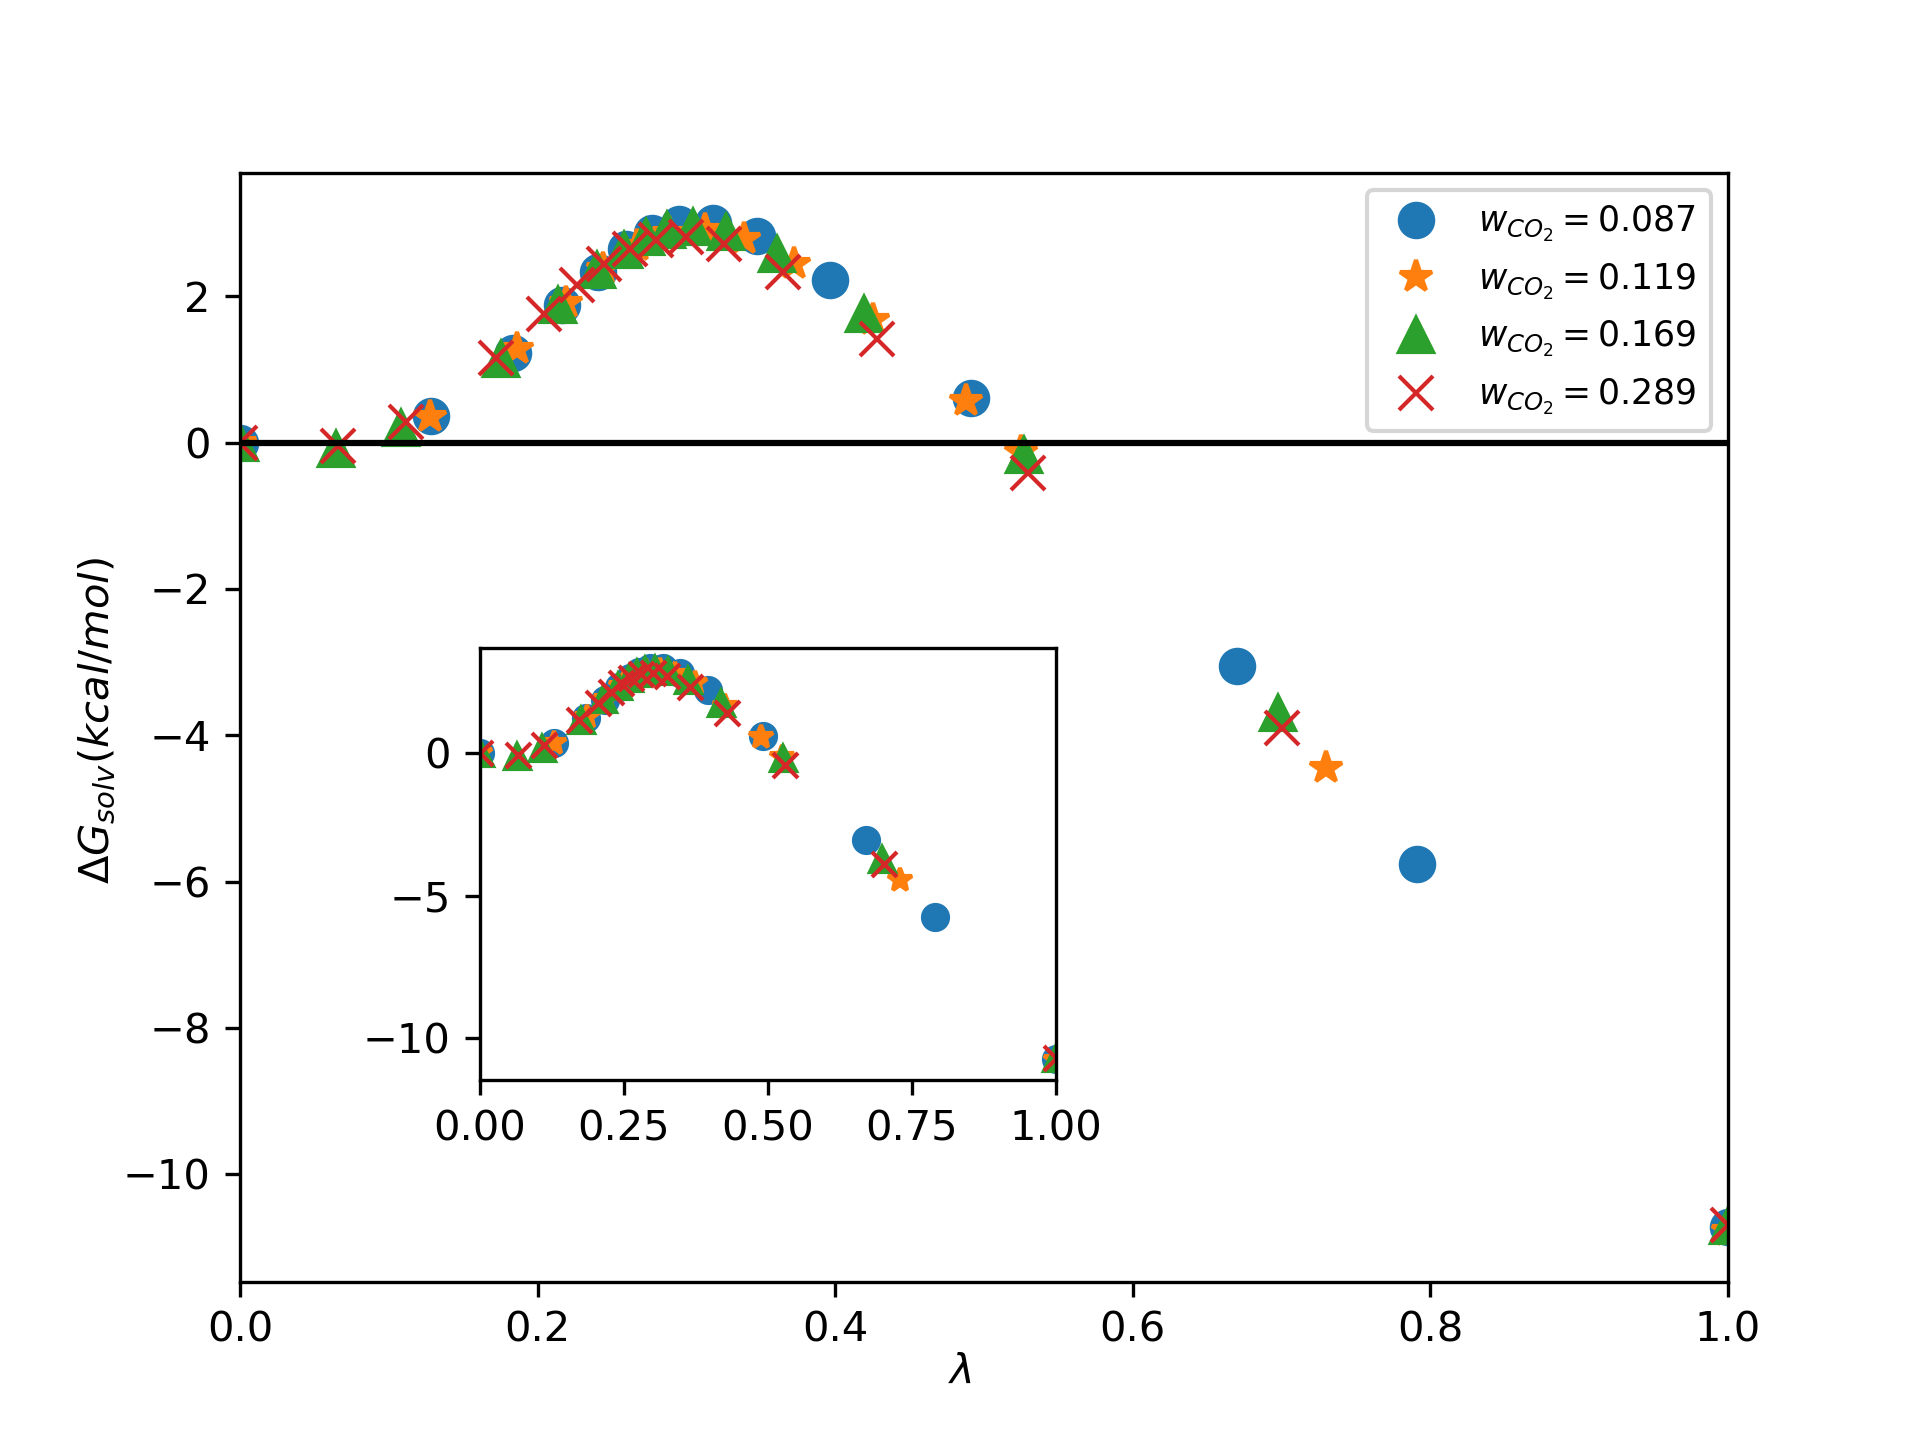
\includegraphics[width=0.8\linewidth]{Figures/tolco2}
	\caption{Representation of solvation free energy profiles obtained with MD simulations of phenanthrene in toluene+$CO_{2}$.}
	\label{fig:Figure_1}
\end{figure}


\section{Hydration free energies}

Water is a solvent extensively used in experimental and computational studies. Because of this importance and the fact that water has unique properties, such as density maximum at 277 K and increased diffusivity upon compression, developing an accurate computational model for water is an ongoing quest \cite{hadley2012}. Hence, we also calculated the solvation free energies in water (hydration free energies) with the SAFT-$\gamma$ Mie force field. With these calculations, we intend to verify if this coarse-grained model would represent the water molecule correctly and would be a good alternative to decrease the computational cost of solvation studies with asphaltene models. The simulations with water as a solvent were carried out using widely studied solutes (propane, benzene) and polyaromatic solutes (toluene, phenanthrene) with a set of fifteen intermediate states.  We obtained these sets of $\lambda$ and $\eta$ with the same methodology used to acquire the sets for the solvation free energies with non-aqueous solvents, and they are exposed in Table \ref{tbl:lambdawater}. At first in our simulations, the binary interaction parameters of all aqueous mixtures were set to zero, but preliminary results for hydration free energies, displayed in Table \ref{tbl:solv3},  exhibited a high deviation from experimental data \cite{P29900000291, doi:10.1021/ct050097l}.

\FloatBarrier
\begin{table*}[h]
	\centering
	\caption{Optimized values of $\lambda $ and $\eta $ for the water+solute pairs. }
	\label{tbl:lambdawater}
	\begin{tabular}{llllllll}
		\hline\hline
		\multicolumn{2}{c}{propane}& \multicolumn{2}{c}{benzene}& \multicolumn{2}{c}{toluene}& \multicolumn{2}{c}{phenanthrene}\\
		\hline\hline
		$\lambda$ & $\eta$ & $\lambda$ & $\eta$  & $\lambda$ & $\eta$  & $\lambda$ & $\eta$ \\ 
		\hline\hline
		0.000    &    0.000    &    0.000    &    0.000    &    0.000    &    0.000    &    0.000    &    0.000    \\
		0.107    &    2.673    &    0.193    &    -0.295    &    0.177    &    0.182    &    0.142    &    -2.462    \\
		0.157    &    4.703    &    0.279    &    1.468    &    0.262    &    2.432    &    0.256    &    0.597    \\
		0.186    &    6.047    &    0.324    &    2.931    &    0.307    &    4.244    &    0.319    &    4.504    \\
		0.210    &    7.148    &    0.357    &    4.168    &    0.336    &    5.552    &    0.358    &    7.762    \\
		0.230    &    8.017    &    0.381    &    5.091    &    0.360    &    6.696    &    0.384    &    10.104    \\
		0.250    &    8.883    &    0.405    &    5.891    &    0.380    &    7.558    &    0.407    &    12.185    \\
		0.272    &    9.291    &    0.427    &    6.443    &    0.400    &    8.233    &    0.427    &    13.607    \\
		0.294    &    9.700    &    0.449    &    6.770    &    0.422    &    8.678    &    0.446    &    14.490    \\
		0.328    &    9.900    &    0.476    &    6.900    &    0.443    &    8.859    &    0.469    &    14.834    \\
		0.381    &    9.930    &    0.506    &    6.805    &    0.473    &    8.810    &    0.494    &    14.667    \\
		0.484    &    9.463    &    0.555    &    6.392    &    0.514    &    8.452    &    0.533    &    13.832    \\
		0.623    &    8.195    &    0.653    &    5.109    &    0.606    &    7.148    &    0.620    &    11.069    \\
		0.781    &    6.378    &    0.810    &    2.421    &    0.755    &    4.273    &    0.806    &    3.279    \\
		1.000    &    3.333    &    1.000    &    -1.480    &    1.000    &    -1.547    &    1.000    &    -6.122    \\        
		\hline\hline
	\end{tabular}
\end{table*}

\begin{table*}[h]
	\centering
	\caption{Calculated values using $k_{ij}=0$ and experimental values for the hydration free energies (kcal/mol) of solutes in water.}
	\label{tbl:solv3}
	\begin{tabular}{cccc}
		\hline\hline
		Solute       & $\Delta G_{solv}^{exp}$ & $\Delta G_{solv}^{Mie}$ & Absolute Deviation \\ \hline\hline
		propane      & $\,$ 2.00 $\pm$ 0.20         & $\,$ 1.10 $\,$ $\pm$ 0.01         & 0.90               \\
		benzene      & -0.86 $\pm$ 0.20        & -4.45 $\, \,$ $\pm$ 0.03        & 3.59               \\
		toluene      & -0.83 $\pm$ 0.20        & -10.98 $\pm$ 0.30       & 10.15              \\
		phenanthrene & -3.88 $\pm$ 0.60        & -10.90 $\pm$ 0.04       & 7.02               \\ \hline\hline
	\end{tabular}
\end{table*}
\FloatBarrier

With these results, the need for binary interaction parameters became clear. First, we estimated $k_{ij}$ with the SAFT-VR Mie EoS and experimental vapor pressure data, but this strategy also provided results that had high absolute deviations from the experimental data. Therefore, we used the approach of estimating the $k_{ij}$ with the output from solvation free energy calculations with molecular dynamics, as described in the last paragraph of Section \ref{solvme}.  We initially found individual values for the interaction parameter of each pair, but, since the parameters for aromatic solutes were very similar (0.148, 0.162, 0.152), we averaged these values. By doing that,  we obtained a general parameter for the water+aromatic pairs, which is exposed in Table \ref{tbl:kij}. Also in this table, we display the binary interaction parameter for the pair water+propane. 

\begin{table*}[h]
	\centering
	\caption{Binary interaction parameters employed.}
	\label{tbl:kij}
	\begin{tabular}{cc}
		\hline
		\hline
		Pair & $k_{ij}$ \\
		\hline\hline
		water+propane      & 0.067  \\
		water+aromatic      & 0.154 \\  
		\hline
		\hline
	\end{tabular}
\end{table*}

The relatively large $k_{ij}$ value of the interaction between aromatic solutes and water can be related to the lack of an explicit association term in the equation of state used to obtain the parameters for water. Actually, the SAFT-VR Mie has an association term \cite{lafitte2013}, but it was not incorporated in the force field. The SAFT-$\gamma$ Mie model for water \cite{lobanova2016} has two different temperature-dependent sets of parameters. The parameters utilized in this work were those estimated with experimental interfacial tension data. Hence, we tested the only binary interaction parameter for water+toluene estimated with MD interfacial data available in the literature \cite{herdes2017}. Nevertheless, the result also had a high absolute deviation, and this parameter could not be transferred to the calculation of the solvation free energy of toluene in water. 

These issues faced by SAFT-$\gamma$ Mie model can also be related to the problems of modeling water with a coarse-grained force field. One of the main difficulties is the choice of which water molecules are going to be represented by which specific beads since water molecules move independently and are only bound by non-bonded interactions \cite{hadley2010,hadley2012}. The  SAFT-$\gamma$ Mie water considers that one water molecule corresponds to one bead. This strategy only saves a small amount of simulation time, but it can predict properties at physiological temperatures unlike other more aggressive models such as the MARTINI, which consider that one bead represents various water molecules. In light of all these problems related to modeling the water molecule, the SAFT-$\gamma$ Mie force field appears to be a good alternative when working close to room temperatures, but the necessity of additional parameters estimated with molecular simulation indicates severe flaws in the methodology. This estimation of the binary parameter increased significantly the simulation time required to calculate the hydration free energies, since we had to carry out three additional simulations for every pair water-solute and then more three additional simulations for the three water+polyaromatic solutes in order to test the averaged binary interaction parameter. If these simulations are necessary for every time a new mixture with water is going to be studied with the SAFT-$\gamma$ Mie force field, the use of this model can become impractical.  With this idea in mind, a useful investigation to be made is to check how much other pairs of water+aromatic solute can be modeled using the binary interaction parameter estimated here. Using these binary interaction parameters calculated with data from molecular dynamics, we then obtained the final hydration free energies presented in Table \ref{tbl:solv2}. 

\begin{table}[H]
	\centering
	\caption{Calculated and experimental hydration free energies  (kcal/mol) of solutes in water.}
	\label{tbl:solv2}
	\begin{tabular}{cccccc}
		\hline\hline
		Solute       & $\Delta G_{solv}^{GAFF}$ & $\Delta G_{solv}^{ELBA}$ & $\Delta G_{solv}^{exp}$ & $\Delta G_{solv}^{Mie}$ & Absolute  \\
		&                          &                          &                         &                         & Deviation \\ \hline\hline
		propane      & 2.50 $\, \pm$0.02           & 2.76 $\, \pm$ 0.02          & 2.00 $\, \pm$ 0.20         & 2.01 $ \, \pm$ 0.01         & 0.01      \\
		benzene      & -0.81$\pm$0.02           & -0.69 $\pm$ 0.01         & -0.86 $\pm$ 0.20        & -1.12 $\pm$ 0.01        & 0.26      \\
		toluene      & -0.79$\pm$0.03           & -0.76 $\pm$ 0.01         & -0.83 $\pm$ 0.20        & -0.84 $\pm$ 0.01        & 0.01      \\
		phenanthrene & -5.26$\pm$0.03           & N/A                        & -3.88 $\pm$ 0.60        & -3.47 $\pm$ 0.02        & 0.41      \\ \hline\hline
		%    RMSE    &                          &                          & 0.24                    &  \\
		%    \hline  &
	\end{tabular}
	
\end{table}

Hydration free energies calculated using the SAFT-$\gamma$ Mie force field with $k_{ij} \neq 0$ had low absolute deviations from the experimental data, as expected since the parameters were adjusted to fit these experimental data. In the table above, we also show the results obtained by \citeonline{doi:10.1021/acs.jctc.5b00963} with the ELBA force field and by \citeonline{PMID:24928188} with the GAFF force field for the solutes and with the TIP3P model for water. The GAFF (General Amber Force Field) force field is an all-atom model that consists of bonded and non-bonded parameters and is suitable for the study of a significant number of molecules. In turn, the TIP3P model considers that water is a rigid monomer represented by three interacting sites with non-bonded interactions and Coulombic interactions \cite{doi:10.1063/1.445869}. Both the GAFF and the TIP3P models use the Lennard-Jones potential to calculate the non-bonded interactions.

Comparing the three mentioned force fields, the root mean square error (RMSE) of all the pairs tested with the SAFT-$\gamma$ Mie model was  0.24, the RMSE for hydration free energies obtained with the GAFF force field was 0.73, and that for the ELBA coarse-grained force field was 0.44. The difference in absolute deviations between the GAFF and SAFT-$\gamma$ Mie force fields is significantly high for phenanthrene, hence the coarse-grained force field with a binary parameter is preferred if the application requires a high level of accuracy. The results also indicated that the SAFT-$\gamma$ Mie model with the binary interaction parameter performed better than the ELBA force field in modeling the solvation phenomenon of the pairs studied in this work, but performed worse with the binary parameter set to zero. This difference in performance occurred despite the fact that both the SAFT-$\gamma$ Mie and ELBA models have the same level of coarse-graining for the solvent (one bead represents one water molecule). Therefore, the choice between the two coarse-grained models is dependent on the availability and transferability of binary interaction parameters of the Mie Model. We also present, for the SAFT-$\gamma$ Mie force field, the hydration free energy profiles in Figure \ref{fig:water}. Bigger molecules had steeper free energy profiles, as it was for the solvation free energy study in other solvents. We also observe that the hydration free energy for the first non-zero $\lambda$ is negative for benzene and toluene when a positive value is expected since free energy is required to 'open space' in the solvent for the solute's insertion. This anomaly can be caused by the fact that the attractive term in the Mie potential compensates the need to open space. 

\begin{figure}[H]
	\centering
	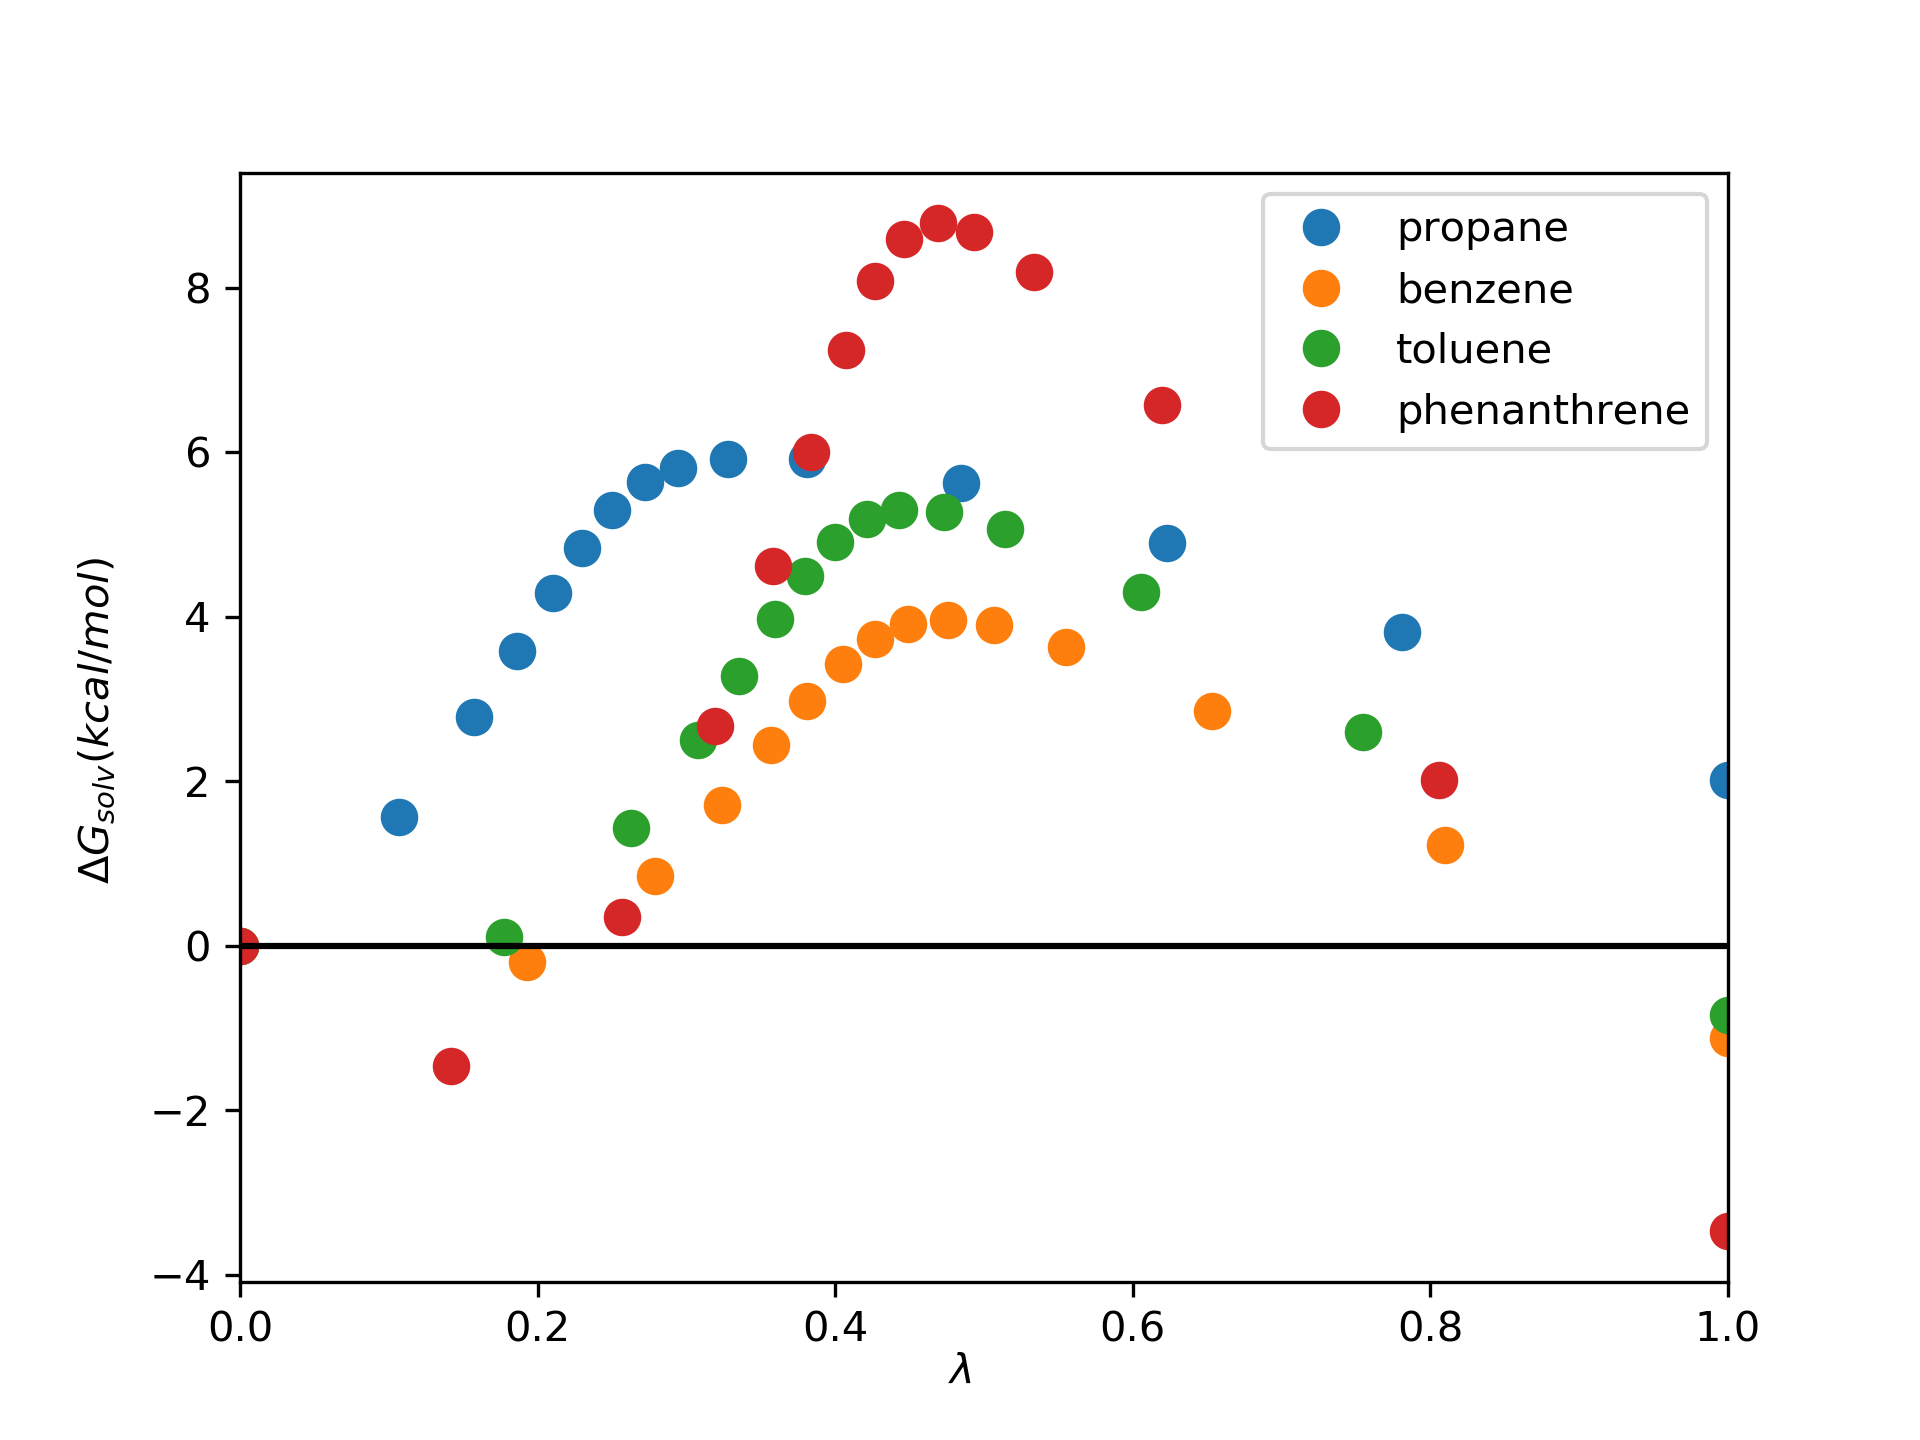
\includegraphics[width=0.8\textwidth]{Figures/water}
	\caption{Representation of hydration free energies of different solutes correspondent to each alchemical state.}
	\label{fig:water}
\end{figure}

The results found here for both the solvation free energies and hydration free energies fulfilled the intentions of this dissertation. We assessed the prediction capability of the SAFT-$\gamma$ Mie force field and provided satisfactory solvation free energy estimates of PAH's using a coarse-grained force field. In addition to that, we found flaws in the methodology used by the SAFT-$\gamma$ Mie force field to model the water molecule. Hence, these shortcomings of this model can now be addressed, and the force field can even be improved by using other mixing rules to avoid the use of a binary parameter or, even, using hydration free energy estimates in the parameterization of water. These results also encourage us to calculate solvation free energies of more complex molecules mimicking asphaltenes in non-aqueous solvents in future studies.  

\section{Partition Coefficients}

Using the solvation free energies estimated in the sections above, we also calculated partition coefficients by means of Eq. \eqref{eqn:partcoe}, for the pairs  water/1-octanol and water/hexane with the intention of testing the modeling capabilities of SAFT-$\gamma$ Mie force field again. The partition functions studied here have many experimental data available in the literature due to their environmental importance \cite{sangster}. Besides this, the calculations of these specific partition coefficients are relevant because   1-octanol is used to quantify hydrophobicity and can serve as a model for biological lipids and different soils \cite{RUELLE2000457}, and hexane is a model for an apolar, hydrophobic phase. Calculated values and experimental data are shown in Table \ref{tbl:part}. The experimental data of the partition coefficients were taken from   \citeonline{POOLE2000117,sangster} for the coefficient of water/1-octanol and from \citeonline{doi:10.1021/je970112e} for the coefficient of water/hexane. 

\begin{table}[H]
	\centering
	\caption{Partition Coefficient Calculated from MD simulations and from experimental data.}
	\label{tbl:part}
	\begin{tabular}{cccc}
		\hline\hline
		& {Molecular Dynamics} & {Experimental} & Absolute Deviation \\ \hline
		\multicolumn{4}{c}{log $P^{water/1-octanol}$}               \\ \hline
		propane      & 2.47                 & 2.40           & 0.07               \\
		phenanthrene & 3.57                 & 4.46           & 0.89               \\ \hline
		\multicolumn{4}{c}{log $P^{water/hexane}$}                 \\ \hline
		benzene      & 1.93                 & 2.06           & 0.13               \\
		phenanthrene & 4.17                 & 4.49           & 0.32               \\
		%                       \multicolumn{4}{c}{log $P^{tolune/hexane}$}                \\ \hline
		%        pyrene       & -0.67                & -0.97          & 0.30               \\
		%        phenanthrene & -0.47                & -              & -                  \\ 
		\hline\hline
	\end{tabular}
	
\end{table}

Overall absolute deviations were small for pairs with smaller solvation free energy deviations such as propane and benzene. The water/1-octanol partition coefficient of phenanthrene had higher deviation due to the higher deviation of the free energy of solvation of this compound in 1-octanol. Comparing with other force fields, \citeonline{garrido} reported average absolute deviations for the water/1-octanol partition coefficient of 0.4 with the GROMOS 53a6 force field \cite{JCC:JCC20090}, 0.3 for TraPPE, and 0.9 for OPLS-AA/TraPPE force fields. However, they attribute the low deviations of TraPPE to the cancellation of errors between the two solvation free energies. Additionally, \citeonline{doi:10.1021/acs.jctc.5b00963} found average absolute deviations of 0.86 for the water/hexane partition coefficients and of 0.75 for the water/1-octanol partition coefficients with the ELBA coarse-grained force field. At this dissertation, we performed a small study of partition coefficients with the SAFT-$\gamma$ Mie force field. Hence, a larger set would be necessary to do a complete evaluation of the performance of this force field in the prediction of partition coefficients.   
\chapter{Conclusions} % Main chapter title

\label{Chapter6} 

This dissertation consisted of the study of solvation free energy calculations of aromatic solutes in different solvents with the SAFT-$\gamma$ Mie coarse-grained force field. Solvation free energy studies are mostly done using water as a solvent and with all-atom force fields based on the Lennard-Jones potential. Therefore, with this study, we were able to provide data about the capability of a coarse-grained force field based on the Mie Potential in calculating solvation free energy differences. Additionally, the solvation free energy estimations carried out here can help improve the SAFT-$\gamma$  Mie force field since these calculations are helpful in identifying errors in the modeling process. The SAFT-$\gamma$ Mie uses the SAFT-VR Mie EoS in its parameterization, which results in a more straightforward method of obtaining parameters. Following this strategy, the phenanthrene parameters, which were not available in this force field database, were obtained using vapor-liquid equilibrium data and two different ring equations and geometries. However, only the parameters estimated with the ring equation proposed by \citeonline{muller2017} were utilized in the solvation free energy simulations since this equation did not require molecular simulation data in its parameterization.

To perform our expanded ensemble simulations, we optimized the coupling parameters and their respective simulation weights. The resulting potential energies from the expanded ensemble simulations were then served as input to estimate solvation free energy differences with the MBAR method. The results for solvation free energy differences with non-aqueous solvents had absolute deviations to the experimental
data of less than 2.0 kcal/mol, except for the pair 1-octanol+anthracene. We also observed the geometry effect on the free energy curves - larger molecules had steeper curves and more substantial absolute deviations. The influence of carbon dioxide on the solvation free energy of phenanthrene in toluene was found to be negligible according to the SAFT-$\gamma$ Mie force field. 

Hydration free energy differences calculations with the SAFT-$\gamma$ Mie model required the use of relatively large values of $k_{ij}$ to obtain satisfactory results. We chose to estimate the parameter with the output from molecular dynamics data since the strategy of using the SAFT-VR Mie EoS provided high absolute deviations to the experimental data. This necessity of one additional parameter probably happens due to the lack of a term to account for the hydrogen bond in the EoS that this force field is based and due to the problems associated with the coarse-graining of water molecules. The results with $k_{ij}$ estimated with MD output were satisfactory, the absolute deviations to the experimental data found were smaller than the ones for the GAFF and ELBA force field. We also used the solvation free energies to calculate partition coefficients in water/1-octanol and water/hexane. The absolute deviations to the experimental data obtained were similar to the ones found for all-atom force fields (GROMOS, TraPPE and OPLS-AA/TraPPE) and other coarse-grained force filed (ELBA).

Overall, the SAFT-$\gamma$ Mie force field proved to be an excellent model to represent the solvation phenomenon of non-aqueous solvents. It correctly described solvation free energy differences of solutes mimicking asphaltenes in hexane, toluene, 1-octanol. However, the calculation of hydration free energies required the use of a binary interaction parameter estimated with MD output, what increased the simulation time significantly. This fact evidenced flaws in the methodology used by the SAFT-$\gamma$ force field and made us question the feasibility of this model for hydration free energy calculations. Nevertheless, the SAFT-$\gamma$ Mie force field for water used here does not predict freezing at room temperature as other force fields, which is essential for our hydration free energy calculations. Hence, it would be relevant to test if the binary interaction parameter for our aromatic solutes estimated here can be used in hydration free energy calculations of other aromatic solutes. Also based on this dissertation, we have some ideas for future development. We intend to use the SAFT-$\gamma$ Mie force field to model bigger asphaltenes models and, consequently, increase the scale of the simulations we performed. Additionally, we want to develop new methodologies to calculate solubility using solvation free energies.


 
%ideias para revisão da bibliografia:
%tipos de modelo coarse grained
%metodologias de energia livre
%\chapter*[Introdução]{Introdução}
%\addcontentsline{toc}{chapter}{Introdução}
%% ----------------------------------------------------------
%
%Este documento e seu código-fonte são exemplos de referência de uso da classe
%\textsf{abntex2} e do pacote \textsf{abntex2cite}. O documento 
%exemplifica a elaboração de trabalho acadêmico (tese, dissertação e outros do
%gênero) produzido conforme a ABNT NBR 14724:2011 \emph{Informação e documentação
%- Trabalhos acadêmicos - Apresentação}.
%
%A expressão ``Modelo Canônico'' é utilizada para indicar que \abnTeX\ não é
%modelo específico de nenhuma universidade ou instituição, mas que implementa tão
%somente os requisitos das normas da ABNT. Uma lista completa das normas
%observadas pelo \abnTeX\ é apresentada em \citeonline{abntex2classe}.
%
%Sinta-se convidado a participar do projeto \abnTeX! Acesse o site do projeto em
%\url{http://www.abntex.net.br/}. Também fique livre para conhecer,
%estudar, alterar e redistribuir o trabalho do \abnTeX, desde que os arquivos
%modificados tenham seus nomes alterados e que os créditos sejam dados aos
%autores originais, nos termos da ``The \LaTeX\ Project Public
%License''\footnote{\url{http://www.latex-project.org/lppl.txt}}.
%
%Encorajamos que sejam realizadas customizações específicas deste exemplo para
%universidades e outras instituições --- como capas, folha de aprovação, etc.
%Porém, recomendamos que ao invés de se alterar diretamente os arquivos do
%\abnTeX, distribua-se arquivos com as respectivas customizações.
%Isso permite que futuras versões do \abnTeX~não se tornem automaticamente
%incompatíveis com as customizações promovidas. Consulte
%\citeonline{abntex2-wiki-como-customizar} par mais informações.
%
%Este documento deve ser utilizado como complemento dos manuais do \abnTeX\ 
%\cite{abntex2classe,abntex2cite,abntex2cite-alf} e da classe \textsf{memoir}
%\cite{memoir}. 
%
%Esperamos, sinceramente, que o \abnTeX\ aprimore a qualidade do trabalho que
%você produzirá, de modo que o principal esforço seja concentrado no principal:
%na contribuição científica.
%
%Equipe \abnTeX 
%
%Lauro César Araujo
%
%% ----------------------------------------------------------
%% PARTE
%% ----------------------------------------------------------
%\part{Preparação da pesquisa}
%% ----------------------------------------------------------
%
%% ---
%% Capitulo com exemplos de comandos inseridos de arquivo externo 
%% ---
%%% abtex2-modelo-include-comandos.tex, v-1.9.6 laurocesar
%% Copyright 2012-2016 by abnTeX2 group at http://www.abntex.net.br/ 
%%
%% This work may be distributed and/or modified under the
%% conditions of the LaTeX Project Public License, either version 1.3
%% of this license or (at your option) any later version.
%% The latest version of this license is in
%%   http://www.latex-project.org/lppl.txt
%% and version 1.3 or later is part of all distributions of LaTeX
%% version 2005/12/01 or later.
%%
%% This work has the LPPL maintenance status `maintained'.
%% 
%% The Current Maintainer of this work is the abnTeX2 team, led
%% by Lauro César Araujo. Further information are available on 
%% http://www.abntex.net.br/
%%
%% This work consists of the files abntex2-modelo-include-comandos.tex
%% and abntex2-modelo-img-marca.pdf
%%

% ---
% Este capítulo, utilizado por diferentes exemplos do abnTeX2, ilustra o uso de
% comandos do abnTeX2 e de LaTeX.
% ---
 
\chapter{Resultados de comandos}\label{cap_exemplos}

\chapterprecis{Isto é uma sinopse de capítulo. A ABNT não traz nenhuma
normatização a respeito desse tipo de resumo, que é mais comum em romances 
e livros técnicos.}\index{sinopse de capítulo}

% ---
\section{Codificação dos arquivos: UTF8}
% ---

A codificação de todos os arquivos do \abnTeX\ é \texttt{UTF8}. É necessário que
você utilize a mesma codificação nos documentos que escrever, inclusive nos
arquivos de base bibliográficas |.bib|.

% ---
\section{Citações diretas}
\label{sec-citacao}
% ---

\index{citações!diretas}Utilize o ambiente \texttt{citacao} para incluir
citações diretas com mais de três linhas:

\begin{citacao}
As citações diretas, no texto, com mais de três linhas, devem ser
destacadas com recuo de 4 cm da margem esquerda, com letra menor que a do texto
utilizado e sem as aspas. No caso de documentos datilografados, deve-se
observar apenas o recuo \cite[5.3]{NBR10520:2002}.
\end{citacao}

Use o ambiente assim:

\begin{verbatim}
\begin{citacao}
As citações diretas, no texto, com mais de três linhas [...] deve-se observar
apenas o recuo \cite[5.3]{NBR10520:2002}.
\end{citacao}
\end{verbatim}

O ambiente \texttt{citacao} pode receber como parâmetro opcional um nome de
idioma previamente carregado nas opções da classe (\autoref{sec-hifenizacao}). Nesse
caso, o texto da citação é automaticamente escrito em itálico e a hifenização é
ajustada para o idioma selecionado na opção do ambiente. Por exemplo:

\begin{verbatim}
\begin{citacao}[english]
Text in English language in italic with correct hyphenation.
\end{citacao}
\end{verbatim}

Tem como resultado:

\begin{citacao}[english]
Text in English language in italic with correct hyphenation.
\end{citacao}

\index{citações!simples}Citações simples, com até três linhas, devem ser
incluídas com aspas. Observe que em \LaTeX as aspas iniciais são diferentes das
finais: ``Amor é fogo que arde sem se ver''.

% ---
\section{Notas de rodapé}
% ---

As notas de rodapé são detalhadas pela NBR 14724:2011 na seção 5.2.1\footnote{As
notas devem ser digitadas ou datilografadas dentro das margens, ficando
separadas do texto por um espaço simples de entre as linhas e por filete de 5
cm, a partir da margem esquerda. Devem ser alinhadas, a partir da segunda linha
da mesma nota, abaixo da primeira letra da primeira palavra, de forma a destacar
o expoente, sem espaço entre elas e com fonte menor
\citeonline[5.2.1]{NBR14724:2011}.}\footnote{Caso uma série de notas sejam
criadas sequencialmente, o \abnTeX\ instrui o \LaTeX\ para que uma vírgula seja
colocada após cada número do expoente que indica a nota de rodapé no corpo do
texto.}\footnote{Verifique se os números do expoente possuem uma vírgula para
dividi-los no corpo do texto.}. 


% ---
\section{Tabelas}
% ---

\index{tabelas}A \autoref{tab-nivinv} é um exemplo de tabela construída em
\LaTeX.

\begin{table}[htb]
\ABNTEXfontereduzida
\caption[Níveis de investigação]{Níveis de investigação.}
\label{tab-nivinv}
\begin{tabular}{p{2.6cm}|p{6.0cm}|p{2.25cm}|p{3.40cm}}
  %\hline
   \textbf{Nível de Investigação} & \textbf{Insumos}  & \textbf{Sistemas de Investigação}  & \textbf{Produtos}  \\
    \hline
    Meta-nível & Filosofia\index{filosofia} da Ciência  & Epistemologia &
    Paradigma  \\
    \hline
    Nível do objeto & Paradigmas do metanível e evidências do nível inferior &
    Ciência  & Teorias e modelos \\
    \hline
    Nível inferior & Modelos e métodos do nível do objeto e problemas do nível inferior & Prática & Solução de problemas  \\
   % \hline
\end{tabular}
\legend{Fonte: \citeonline{van86}}
\end{table}

Já a \autoref{tabela-ibge} apresenta uma tabela criada conforme o padrão do
\citeonline{ibge1993} requerido pelas normas da ABNT para documentos técnicos e
acadêmicos.

\begin{table}[htb]
\IBGEtab{%
  \caption{Um Exemplo de tabela alinhada que pode ser longa
  ou curta, conforme padrão IBGE.}%
  \label{tabela-ibge}
}{%
  \begin{tabular}{ccc}
  \toprule
   Nome & Nascimento & Documento \\
  \midrule \midrule
   Maria da Silva & 11/11/1111 & 111.111.111-11 \\
  \midrule 
   João Souza & 11/11/2111 & 211.111.111-11 \\
  \midrule 
   Laura Vicuña & 05/04/1891 & 3111.111.111-11 \\
  \bottomrule
\end{tabular}%
}{%
  \fonte{Produzido pelos autores.}%
  \nota{Esta é uma nota, que diz que os dados são baseados na
  regressão linear.}%
  \nota[Anotações]{Uma anotação adicional, que pode ser seguida de várias
  outras.}%
  }
\end{table}


% ---
\section{Figuras}
% ---

\index{figuras}Figuras podem ser criadas diretamente em \LaTeX,
como o exemplo da \autoref{fig_circulo}.

\begin{figure}[htb]
	\caption{\label{fig_circulo}A delimitação do espaço}
	\begin{center}
	    \setlength{\unitlength}{5cm}
		\begin{picture}(1,1)
		\put(0,0){\line(0,1){1}}
		\put(0,0){\line(1,0){1}}
		\put(0,0){\line(1,1){1}}
		\put(0,0){\line(1,2){.5}}
		\put(0,0){\line(1,3){.3333}}
		\put(0,0){\line(1,4){.25}}
		\put(0,0){\line(1,5){.2}}
		\put(0,0){\line(1,6){.1667}}
		\put(0,0){\line(2,1){1}}
		\put(0,0){\line(2,3){.6667}}
		\put(0,0){\line(2,5){.4}}
		\put(0,0){\line(3,1){1}}
		\put(0,0){\line(3,2){1}}
		\put(0,0){\line(3,4){.75}}
		\put(0,0){\line(3,5){.6}}
		\put(0,0){\line(4,1){1}}
		\put(0,0){\line(4,3){1}}
		\put(0,0){\line(4,5){.8}}
		\put(0,0){\line(5,1){1}}
		\put(0,0){\line(5,2){1}}
		\put(0,0){\line(5,3){1}}
		\put(0,0){\line(5,4){1}}
		\put(0,0){\line(5,6){.8333}}
		\put(0,0){\line(6,1){1}}
		\put(0,0){\line(6,5){1}}
		\end{picture}
	\end{center}
	\legend{Fonte: os autores}
\end{figure}

Ou então figuras podem ser incorporadas de arquivos externos, como é o caso da
\autoref{fig_grafico}. Se a figura que ser incluída se tratar de um diagrama, um
gráfico ou uma ilustração que você mesmo produza, priorize o uso de imagens
vetoriais no formato PDF. Com isso, o tamanho do arquivo final do trabalho será
menor, e as imagens terão uma apresentação melhor, principalmente quando
impressas, uma vez que imagens vetorias são perfeitamente escaláveis para
qualquer dimensão. Nesse caso, se for utilizar o Microsoft Excel para produzir
gráficos, ou o Microsoft Word para produzir ilustrações, exporte-os como PDF e
os incorpore ao documento conforme o exemplo abaixo. No entanto, para manter a
coerência no uso de software livre (já que você está usando \LaTeX e \abnTeX),
teste a ferramenta \textsf{InkScape}\index{InkScape}
(\url{http://inkscape.org/}). Ela é uma excelente opção de código-livre para
produzir ilustrações vetoriais, similar ao CorelDraw\index{CorelDraw} ou ao Adobe
Illustrator\index{Adobe Illustrator}. De todo modo, caso não seja possível
utilizar arquivos de imagens como PDF, utilize qualquer outro formato, como
JPEG, GIF, BMP, etc. Nesse caso, você pode tentar aprimorar as imagens
incorporadas com o software livre \textsf{Gimp}\index{Gimp}
(\url{http://www.gimp.org/}). Ele é uma alternativa livre ao Adobe
Photoshop\index{Adobe Photoshop}.

\begin{figure}[htb]
	\caption{\label{fig_grafico}Gráfico produzido em Excel e salvo como PDF}
	\begin{center}
	    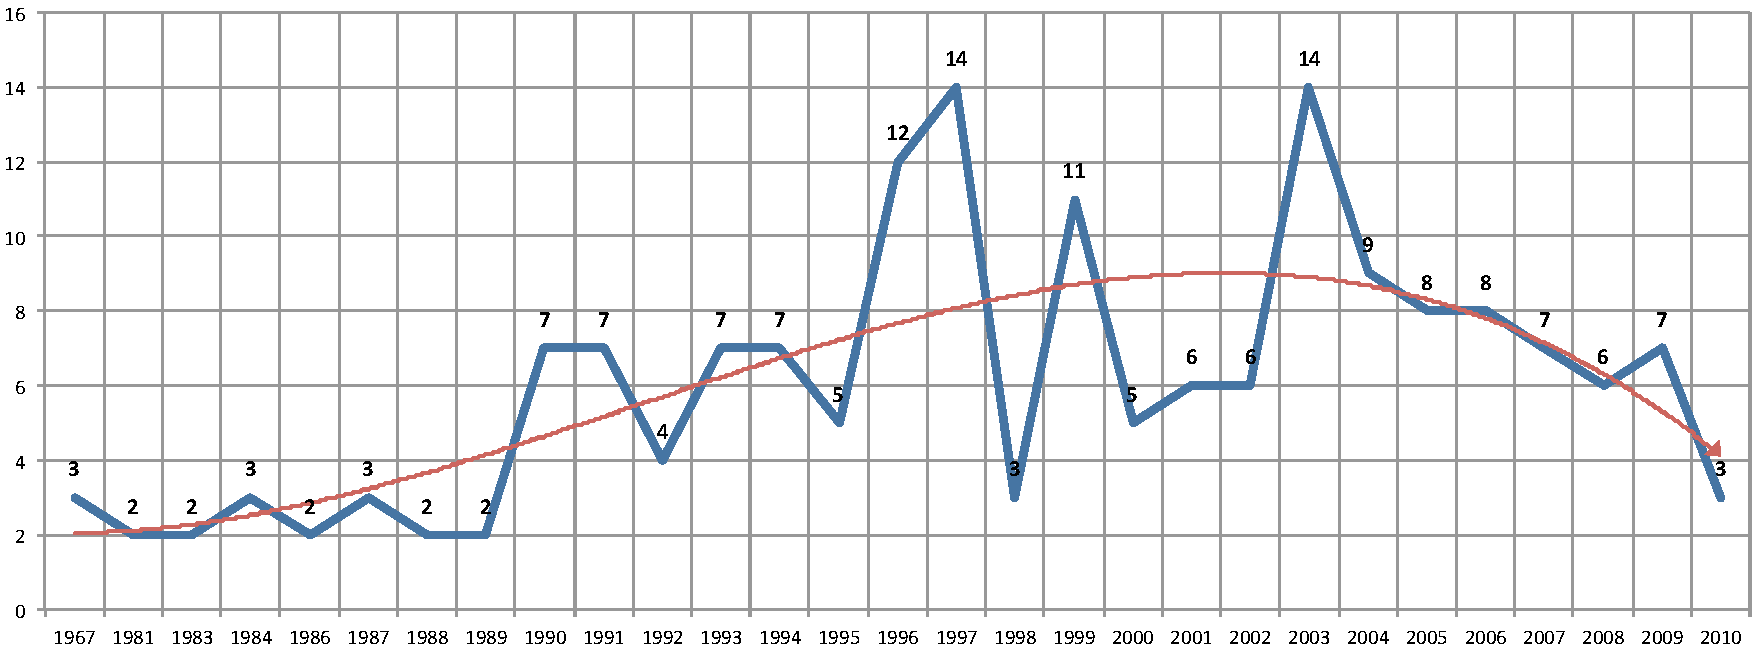
\includegraphics[scale=0.5]{abntex2-modelo-img-grafico.pdf}
	\end{center}
	\legend{Fonte: \citeonline[p. 24]{araujo2012}}
\end{figure}

% ---
\subsection{Figuras em \emph{minipages}}
% ---

\emph{Minipages} são usadas para inserir textos ou outros elementos em quadros
com tamanhos e posições controladas. Veja o exemplo da
\autoref{fig_minipage_imagem1} e da \autoref{fig_minipage_grafico2}.

\begin{figure}[htb]
 \label{teste}
 \centering
  \begin{minipage}{0.4\textwidth}
    \centering
    \caption{Imagem 1 da minipage} \label{fig_minipage_imagem1}
    
\includegraphics[scale=0.9]{abntex2-modelo-img-marca.pdf}
    \legend{Fonte: Produzido pelos autores}
  \end{minipage}
  \hfill
  \begin{minipage}{0.4\textwidth}
    \centering
    \caption{Grafico 2 da minipage} \label{fig_minipage_grafico2}
    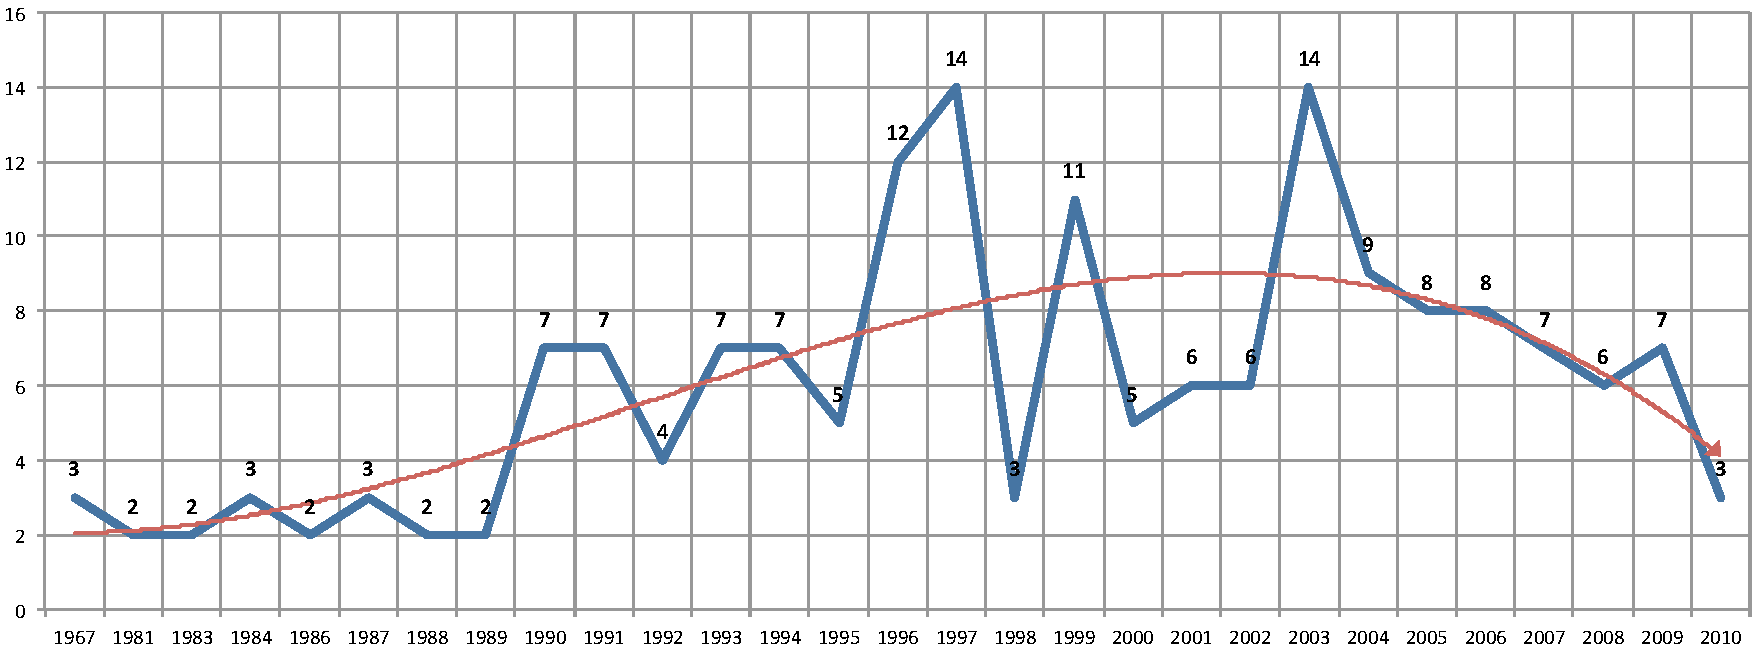
\includegraphics[scale=0.2]{abntex2-modelo-img-grafico.pdf}
    \legend{Fonte: \citeonline[p. 24]{araujo2012}}
  \end{minipage}
\end{figure}

Observe que, segundo a \citeonline[seções 4.2.1.10 e 5.8]{NBR14724:2011}, as
ilustrações devem sempre ter numeração contínua e única em todo o documento:

\begin{citacao}
Qualquer que seja o tipo de ilustração, sua identificação aparece na parte
superior, precedida da palavra designativa (desenho, esquema, fluxograma,
fotografia, gráfico, mapa, organograma, planta, quadro, retrato, figura,
imagem, entre outros), seguida de seu número de ordem de ocorrência no texto,
em algarismos arábicos, travessão e do respectivo título. Após a ilustração, na
parte inferior, indicar a fonte consultada (elemento obrigatório, mesmo que
seja produção do próprio autor), legenda, notas e outras informações
necessárias à sua compreensão (se houver). A ilustração deve ser citada no
texto e inserida o mais próximo possível do trecho a que se
refere. \cite[seções 5.8]{NBR14724:2011}
\end{citacao}

% ---
\section{Expressões matemáticas}
% ---

\index{expressões matemáticas}Use o ambiente \texttt{equation} para escrever
expressões matemáticas numeradas:

\begin{equation}
  \forall x \in X, \quad \exists \: y \leq \epsilon
\end{equation}

Escreva expressões matemáticas entre \$ e \$, como em $ \lim_{x \to \infty}
\exp(-x) = 0 $, para que fiquem na mesma linha.

Também é possível usar colchetes para indicar o início de uma expressão
matemática que não é numerada.

\[
\left|\sum_{i=1}^n a_ib_i\right|
\le
\left(\sum_{i=1}^n a_i^2\right)^{1/2}
\left(\sum_{i=1}^n b_i^2\right)^{1/2}
\]

Consulte mais informações sobre expressões matemáticas em
\url{https://github.com/abntex/abntex2/wiki/Referencias}.

% ---
\section{Enumerações: alíneas e subalíneas}
% ---

\index{alíneas}\index{subalíneas}\index{incisos}Quando for necessário enumerar
os diversos assuntos de uma seção que não possua título, esta deve ser
subdividida em alíneas \cite[4.2]{NBR6024:2012}:

\begin{alineas}

  \item os diversos assuntos que não possuam título próprio, dentro de uma mesma
  seção, devem ser subdivididos em alíneas; 
  
  \item o texto que antecede as alíneas termina em dois pontos;
  \item as alíneas devem ser indicadas alfabeticamente, em letra minúscula,
  seguida de parêntese. Utilizam-se letras dobradas, quando esgotadas as
  letras do alfabeto;

  \item as letras indicativas das alíneas devem apresentar recuo em relação à
  margem esquerda;

  \item o texto da alínea deve começar por letra minúscula e terminar em
  ponto-e-vírgula, exceto a última alínea que termina em ponto final;

  \item o texto da alínea deve terminar em dois pontos, se houver subalínea;

  \item a segunda e as seguintes linhas do texto da alínea começa sob a
  primeira letra do texto da própria alínea;
  
  \item subalíneas \cite[4.3]{NBR6024:2012} devem ser conforme as alíneas a
  seguir:

  \begin{alineas}
     \item as subalíneas devem começar por travessão seguido de espaço;

     \item as subalíneas devem apresentar recuo em relação à alínea;

     \item o texto da subalínea deve começar por letra minúscula e terminar em
     ponto-e-vírgula. A última subalínea deve terminar em ponto final, se não
     houver alínea subsequente;

     \item a segunda e as seguintes linhas do texto da subalínea começam sob a
     primeira letra do texto da própria subalínea.
  \end{alineas}
  
  \item no \abnTeX\ estão disponíveis os ambientes \texttt{incisos} e
  \texttt{subalineas}, que em suma são o mesmo que se criar outro nível de
  \texttt{alineas}, como nos exemplos à seguir:
  
  \begin{incisos}
    \item \textit{Um novo inciso em itálico};
  \end{incisos}
  
  \item Alínea em \textbf{negrito}:
  
  \begin{subalineas}
    \item \textit{Uma subalínea em itálico};
    \item \underline{\textit{Uma subalínea em itálico e sublinhado}}; 
  \end{subalineas}
  
  \item Última alínea com \emph{ênfase}.
  
\end{alineas}

% ---
\section{Espaçamento entre parágrafos e linhas}
% ---

\index{espaçamento!dos parágrafos}O tamanho do parágrafo, espaço entre a margem
e o início da frase do parágrafo, é definido por:

\begin{verbatim}
   \setlength{\parindent}{1.3cm}
\end{verbatim}

\index{espaçamento!do primeiro parágrafo}Por padrão, não há espaçamento no
primeiro parágrafo de cada início de divisão do documento
(\autoref{sec-divisoes}). Porém, você pode definir que o primeiro parágrafo
também seja indentado, como é o caso deste documento. Para isso, apenas inclua o
pacote \textsf{indentfirst} no preâmbulo do documento:

\begin{verbatim}
   \usepackage{indentfirst}      % Indenta o primeiro parágrafo de cada seção.
\end{verbatim}

\index{espaçamento!entre os parágrafos}O espaçamento entre um parágrafo e outro
pode ser controlado por meio do comando:

\begin{verbatim}
  \setlength{\parskip}{0.2cm}  % tente também \onelineskip
\end{verbatim}

\index{espaçamento!entre as linhas}O controle do espaçamento entre linhas é
definido por:

\begin{verbatim}
  \OnehalfSpacing       % espaçamento um e meio (padrão); 
  \DoubleSpacing        % espaçamento duplo
  \SingleSpacing        % espaçamento simples	
\end{verbatim}

Para isso, também estão disponíveis os ambientes:

\begin{verbatim}
  \begin{SingleSpace} ...\end{SingleSpace}
  \begin{Spacing}{hfactori} ... \end{Spacing}
  \begin{OnehalfSpace} ... \end{OnehalfSpace}
  \begin{OnehalfSpace*} ... \end{OnehalfSpace*}
  \begin{DoubleSpace} ... \end{DoubleSpace}
  \begin{DoubleSpace*} ... \end{DoubleSpace*} 
\end{verbatim}

Para mais informações, consulte \citeonline[p. 47-52 e 135]{memoir}.

% ---
\section{Inclusão de outros arquivos}\label{sec-include}
% ---

É uma boa prática dividir o seu documento em diversos arquivos, e não
apenas escrever tudo em um único. Esse recurso foi utilizado neste
documento. Para incluir diferentes arquivos em um arquivo principal,
de modo que cada arquivo incluído fique em uma página diferente, utilize o
comando:

\begin{verbatim}
   \include{documento-a-ser-incluido}      % sem a extensão .tex
\end{verbatim}

Para incluir documentos sem quebra de páginas, utilize:

\begin{verbatim}
   \input{documento-a-ser-incluido}      % sem a extensão .tex
\end{verbatim}

% ---
\section{Compilar o documento \LaTeX}
% ---

Geralmente os editores \LaTeX, como o
TeXlipse\footnote{\url{http://texlipse.sourceforge.net/}}, o
Texmaker\footnote{\url{http://www.xm1math.net/texmaker/}}, entre outros,
compilam os documentos automaticamente, de modo que você não precisa se
preocupar com isso.

No entanto, você pode compilar os documentos \LaTeX usando os seguintes
comandos, que devem ser digitados no \emph{Prompt de Comandos} do Windows ou no
\emph{Terminal} do Mac ou do Linux:

\begin{verbatim}
   pdflatex ARQUIVO_PRINCIPAL.tex
   bibtex ARQUIVO_PRINCIPAL.aux
   makeindex ARQUIVO_PRINCIPAL.idx 
   makeindex ARQUIVO_PRINCIPAL.nlo -s nomencl.ist -o ARQUIVO_PRINCIPAL.nls
   pdflatex ARQUIVO_PRINCIPAL.tex
   pdflatex ARQUIVO_PRINCIPAL.tex
\end{verbatim}

% ---
\section{Remissões internas}
% ---

Ao nomear a \autoref{tab-nivinv} e a \autoref{fig_circulo}, apresentamos um
exemplo de remissão interna, que também pode ser feita quando indicamos o
\autoref{cap_exemplos}, que tem o nome \emph{\nameref{cap_exemplos}}. O número
do capítulo indicado é \ref{cap_exemplos}, que se inicia à
\autopageref{cap_exemplos}\footnote{O número da página de uma remissão pode ser
obtida também assim:
\pageref{cap_exemplos}.}.
Veja a \autoref{sec-divisoes} para outros exemplos de remissões internas entre
seções, subseções e subsubseções.

O código usado para produzir o texto desta seção é:

\begin{verbatim}
Ao nomear a \autoref{tab-nivinv} e a \autoref{fig_circulo}, apresentamos um
exemplo de remissão interna, que também pode ser feita quando indicamos o
\autoref{cap_exemplos}, que tem o nome \emph{\nameref{cap_exemplos}}. O número
do capítulo indicado é \ref{cap_exemplos}, que se inicia à
\autopageref{cap_exemplos}\footnote{O número da página de uma remissão pode ser
obtida também assim:
\pageref{cap_exemplos}.}.
Veja a \autoref{sec-divisoes} para outros exemplos de remissões internas entre
seções, subseções e subsubseções.
\end{verbatim}

% ---
\section{Divisões do documento: seção}\label{sec-divisoes}
% ---

Esta seção testa o uso de divisões de documentos. Esta é a
\autoref{sec-divisoes}. Veja a \autoref{sec-divisoes-subsection}.

\subsection{Divisões do documento: subseção}\label{sec-divisoes-subsection}

Isto é uma subseção. Veja a \autoref{sec-divisoes-subsubsection}, que é uma
\texttt{subsubsection} do \LaTeX, mas é impressa chamada de ``subseção'' porque
no Português não temos a palavra ``subsubseção''.

\subsubsection{Divisões do documento: subsubseção}
\label{sec-divisoes-subsubsection}

Isto é uma subsubseção.

\subsubsection{Divisões do documento: subsubseção}

Isto é outra subsubseção.

\subsection{Divisões do documento: subseção}\label{sec-exemplo-subsec}

Isto é uma subseção.

\subsubsection{Divisões do documento: subsubseção}

Isto é mais uma subsubseção da \autoref{sec-exemplo-subsec}.


\subsubsubsection{Esta é uma subseção de quinto
nível}\label{sec-exemplo-subsubsubsection}

Esta é uma seção de quinto nível. Ela é produzida com o seguinte comando:

\begin{verbatim}
\subsubsubsection{Esta é uma subseção de quinto
nível}\label{sec-exemplo-subsubsubsection}
\end{verbatim}

\subsubsubsection{Esta é outra subseção de quinto nível}\label{sec-exemplo-subsubsubsection-outro}

Esta é outra seção de quinto nível.


\paragraph{Este é um parágrafo numerado}\label{sec-exemplo-paragrafo}

Este é um exemplo de parágrafo nomeado. Ele é produzida com o comando de
parágrafo:

\begin{verbatim}
\paragraph{Este é um parágrafo nomeado}\label{sec-exemplo-paragrafo}
\end{verbatim}

A numeração entre parágrafos numeradaos e subsubsubseções são contínuas.

\paragraph{Esta é outro parágrafo numerado}\label{sec-exemplo-paragrafo-outro}

Esta é outro parágrafo nomeado.

% ---
\section{Este é um exemplo de nome de seção longo. Ele deve estar
alinhado à esquerda e a segunda e demais linhas devem iniciar logo abaixo da
primeira palavra da primeira linha}
% ---

Isso atende à norma \citeonline[seções de 5.2.2 a 5.2.4]{NBR14724:2011} 
 e \citeonline[seções de 3.1 a 3.8]{NBR6024:2012}.

% ---
\section{Diferentes idiomas e hifenizações}
\label{sec-hifenizacao}
% ---

Para usar hifenizações de diferentes idiomas, inclua nas opções do documento o
nome dos idiomas que o seu texto contém. Por exemplo (para melhor
visualização, as opções foram quebras em diferentes linhas):

\begin{verbatim}
\documentclass[
	12pt,
	openright,
	twoside,
	a4paper,
	english,
	brazil
	]{abntex2}
\end{verbatim}

O idioma português-brasileiro (\texttt{brazil}) é incluído automaticamente pela
classe \textsf{abntex2}. Porém, mesmo assim a opção \texttt{brazil} deve ser
informada como a última opção da classe para que todos os pacotes reconheçam o
idioma. Vale ressaltar que a última opção de idioma é a utilizada por padrão no
documento. Desse modo, caso deseje escrever um texto em inglês que tenha
citações em português e em francês, você deveria usar o preâmbulo como abaixo:

\begin{verbatim}
\documentclass[
	12pt,
	openright,
	twoside,
	a4paper,
	brazil,
	english
	]{abntex2}
\end{verbatim}

A lista completa de idiomas suportados, bem como outras opções de hifenização,
estão disponíveis em \citeonline[p.~5-6]{babel}.

Exemplo de hifenização em inglês\footnote{Extraído de:
\url{http://en.wikibooks.org/wiki/LaTeX/Internationalization}}:

\begin{otherlanguage*}{english}
\textit{Text in English language. This environment switches all language-related
definitions, like the language specific names for figures, tables etc. to the other
language. The starred version of this environment typesets the main text
according to the rules of the other language, but keeps the language specific
string for ancillary things like figures, in the main language of the document.
The environment hyphenrules switches only the hyphenation patterns used; it can
also be used to disallow hyphenation by using the language name
`nohyphenation'.}
\end{otherlanguage*}

Exemplo de hifenização em francês\footnote{Extraído de:
\url{http://bigbrowser.blog.lemonde.fr/2013/02/17/tu-ne-tweeteras-point-le-vatican-interdit-aux-cardinaux-de-tweeter-pendant-le-conclave/}}:


Pequeno texto em espanhol\footnote{Extraído de:
\url{http://internacional.elpais.com/internacional/2013/02/17/actualidad/1361102009_913423.html}}:

O idioma geral do texto por ser alterado como no exemplo seguinte:

\begin{verbatim}
  \selectlanguage{english}
\end{verbatim}

Isso altera automaticamente a hifenização e todos os nomes constantes de
referências do documento para o idioma inglês. Consulte o manual da classe
\cite{abntex2classe} para obter orientações adicionais sobre internacionalização de
documentos produzidos com \abnTeX.

A \autoref{sec-citacao} descreve o ambiente \texttt{citacao} que pode receber
como parâmetro um idioma a ser usado na citação.

% ---
\section{Consulte o manual da classe \textsf{abntex2}}
% ---

Consulte o manual da classe \textsf{abntex2} \cite{abntex2classe} para uma
referência completa das macros e ambientes disponíveis. 

Além disso, o manual possui informações adicionais sobre as normas ABNT
observadas pelo \abnTeX\ e considerações sobre eventuais requisitos específicos
não atendidos, como o caso da \citeonline[seção 5.2.2]{NBR14724:2011}, que
especifica o espaçamento entre os capítulos e o início do texto, regra
propositalmente não atendida pelo presente modelo.

% ---
\section{Referências bibliográficas}
% ---

A formatação das referências bibliográficas conforme as regras da ABNT são um
dos principais objetivos do \abnTeX. Consulte os manuais
\citeonline{abntex2cite} e \citeonline{abntex2cite-alf} para obter informações
sobre como utilizar as referências bibliográficas.

%-
\subsection{Acentuação de referências bibliográficas}
%-

Normalmente não há problemas em usar caracteres acentuados em arquivos
bibliográficos (\texttt{*.bib}). Porém, como as regras da ABNT fazem uso quase
abusivo da conversão para letras maiúsculas, é preciso observar o modo como se
escreve os nomes dos autores. Na ~\autoref{tabela-acentos} você encontra alguns
exemplos das conversões mais importantes. Preste atenção especial para `ç' e `í'
que devem estar envoltos em chaves. A regra geral é sempre usar a acentuação
neste modo quando houver conversão para letras maiúsculas.

\begin{table}[htbp]
\caption{Tabela de conversão de acentuação.}
\label{tabela-acentos}

\begin{center}
\begin{tabular}{ll}\hline\hline
acento & \textsf{bibtex}\\
à á ã & \verb+\`a+ \verb+\'a+ \verb+\~a+\\
í & \verb+{\'\i}+\\
ç & \verb+{\c c}+\\
\hline\hline
\end{tabular}
\end{center}
\end{table}


% ---
\section{Precisa de ajuda?}
% ---

Consulte a FAQ com perguntas frequentes e comuns no portal do \abnTeX:
\url{https://github.com/abntex/abntex2/wiki/FAQ}.

Inscreva-se no grupo de usuários \LaTeX:
\url{http://groups.google.com/group/latex-br}, tire suas dúvidas e ajude
outros usuários.

Participe também do grupo de desenvolvedores do \abnTeX:
\url{http://groups.google.com/group/abntex2} e faça sua contribuição à
ferramenta.

% ---
\section{Você pode ajudar?}
% ---

Sua contribuição é muito importante! Você pode ajudar na divulgação, no
desenvolvimento e de várias outras formas. Veja como contribuir com o \abnTeX\
em \url{https://github.com/abntex/abntex2/wiki/Como-Contribuir}.

% ---
\section{Quer customizar os modelos do \abnTeX\ para sua instituição ou
universidade?}
% ---

Veja como customizar o \abnTeX\ em:
\url{https://github.com/abntex/abntex2/wiki/ComoCustomizar}.


%% ---
%
%% ----------------------------------------------------------
%% PARTE
%% ----------------------------------------------------------
%\part{Referenciais teóricos}
%% ----------------------------------------------------------
%
%% ---
%% Capitulo de revisão de literatura
%% ---
%\chapter{Lorem ipsum dolor sit amet}
%% ---
%
%% ---
%\section{Aliquam vestibulum fringilla lorem}
%% ---
%
%\lipsum[1]
%
%\lipsum[2-3]
%
%% ----------------------------------------------------------
%% PARTE
%% ----------------------------------------------------------
%\part{Resultados}
%% ----------------------------------------------------------
%
%% ---
%% primeiro capitulo de Resultados
%% ---
%\chapter{Lectus lobortis condimentum}
%% ---
%
%% ---
%\section{Vestibulum ante ipsum primis in faucibus orci luctus et ultrices
%posuere cubilia Curae}
%% ---
%
%\lipsum[21-22]
%
%% ---
%% segundo capitulo de Resultados
%% ---
%\chapter{Nam sed tellus sit amet lectus urna ullamcorper tristique interdum
%elementum}
%% ---
%
%% ---
%\section{Pellentesque sit amet pede ac sem eleifend consectetuer}
%% ---
%
%\lipsum[24]
%
%% ----------------------------------------------------------
%% Finaliza a parte no bookmark do PDF
%% para que se inicie o bookmark na raiz
%% e adiciona espaço de parte no Sumário
%% ----------------------------------------------------------
%\phantompart
%
%% ---
%% Conclusão
%% ---
%\chapter{Conclusão}
%% ---
%
%\lipsum[31-33]

% ----------------------------------------------------------
% ELEMENTOS PÓS-TEXTUAIS
% ----------------------------------------------------------
\postextual
% ----------------------------------------------------------

% ----------------------------------------------------------
% Referências bibliográficas
% ----------------------------------------------------------
\bibliography{thesis}

% ----------------------------------------------------------
% Glossário
% ----------------------------------------------------------
%
% Consulte o manual da classe abntex2 para orientações sobre o glossário.
%
%\glossary

% ----------------------------------------------------------
% Apêndices
% ----------------------------------------------------------

% ---
% Inicia os apêndices
% ---
\begin{apendicesenv}

% Imprime uma página indicando o início dos apêndices
\partapendices

% ----------------------------------------------------------
\chapter{Optimized values of $\lambda$ and $\eta$}
% ----------------------------------------------------------
\begin{table*}[h]
	\centering
	\caption{Optimized values of $\lambda$ and $\eta$ for the solutes in hexane}
	\begin{tabular}{llllll}
		\hline
        \multicolumn{2}{c}{benzene}& \multicolumn{2}{c}{pyrene}& \multicolumn{2}{c}{phenanthrene}\\
		\hline
		$\lambda$ & $\eta$ & $\lambda$ & $\eta$  & $\lambda$ & $\eta$   \\ 
		\hline
0.000	&	0.000	&	0.000	&	0.000	&	0.000	&	0.000	\\
0.065	&	0.708	&	0.076	&	4.234	&	0.090	&	1.981	\\
0.112	&	1.385	&	0.107	&	5.620	&	0.132	&	3.461	\\
0.150	&	1.892	&	0.132	&	6.499	&	0.161	&	4.494	\\
0.188	&	2.399	&	0.152	&	6.690	&	0.185	&	5.185	\\
0.226	&	2.519	&	0.170	&	6.643	&	0.205	&	5.552	\\
0.264	&	2.457	&	0.189	&	6.461	&	0.224	&	5.725	\\
0.304	&	2.367	&	0.213	&	6.091	&	0.244	&	5.722	\\
0.356	&	1.921	&	0.242	&	5.566	&	0.268	&	5.523	\\
0.411	&	1.411	&	0.280	&	4.729	&	0.305	&	4.975	\\
0.492	&	0.524	&	0.355	&	2.853	&	0.372	&	3.576	\\
0.588	&	-0.663	&	0.483	&	-0.778	&	0.500	&	0.297	\\
0.690	&	-2.016	&	0.678	&	-6.947	&	0.560	&	-1.390	\\
0.824	&	-3.922	&	0.788	&	-10.631	&	0.722	&	-6.309	\\
1.000	&	-6.583	&	1.000	&	-18.141	&	1.000	&	-15.448	\\

		\hline
	\end{tabular}
\end{table*}

\begin{table*}[h]
	\centering
	\caption{Optimized values of $\lambda$ and $\eta$ for the solutes in 1-octanol}
	\begin{tabular}{llllll}
		\hline
		\multicolumn{2}{c}{propane}& \multicolumn{2}{c}{anthracene}& \multicolumn{2}{c}{phenanthrene}\\
		\hline
		$\lambda$ & $\eta$ & $\lambda$ & $\eta$  & $\lambda$ & $\eta$   \\ 
		\hline
0.000	&	0.000	&	0.000	&	0.000	&	0.000	&	0.000	\\
0.027	&	3.126	&	0.078	&	3.932	&	0.049	&	2.578	\\
0.050	&	5.109	&	0.111	&	6.178	&	0.091	&	5.663	\\
0.073	&	6.093	&	0.130	&	7.426	&	0.125	&	8.575	\\
0.095	&	6.570	&	0.143	&	8.201	&	0.144	&	10.069	\\
0.117	&	6.826	&	0.154	&	8.717	&	0.157	&	10.978	\\
0.142	&	6.956	&	0.164	&	9.085	&	0.169	&	11.599	\\
0.174	&	6.969	&	0.174	&	9.357	&	0.180	&	12.040	\\
0.215	&	6.847	&	0.184	&	9.556	&	0.192	&	12.340	\\
0.269	&	6.554	&	0.197	&	9.676	&	0.206	&	12.499	\\
0.337	&	6.050	&	0.214	&	9.681	&	0.225	&	12.478	\\
0.427	&	5.228	&	0.238	&	9.490	&	0.253	&	12.161	\\
0.545	&	3.955	&	0.274	&	8.958	&	0.298	&	11.280	\\
0.720	&	1.843	&	0.326	&	7.906	&	0.371	&	9.406	\\
1.000	&	-1.903	&	0.399	&	6.088	&	0.484	&	5.891	\\
&		&	0.515	&	2.777	&	0.664	&	-0.516	\\
&		&	0.695	&	-2.960	&	0.802	&	-5.908	\\
&		&	1.000	&	-13.768	&	1.000	&	-14.073	\\

		
		\hline
	\end{tabular}
\end{table*}

\begin{table*}[h]
	\centering
	\caption{Optimized values of $\lambda$ and $\eta$ for the solutes in toluene}
	\begin{tabular}{llllll}
		\hline
		\multicolumn{2}{c}{pyrene}& \multicolumn{2}{c}{anthracene}& \multicolumn{2}{c}{phenanthrene}\\
		\hline
		$\lambda$ & $\eta$ & $\lambda$ & $\eta$  & $\lambda$ & $\eta$   \\ 
		\hline
0.000	&	0.000	&	0.000	&	0.000	&	0.000	&	0.000	\\
0.090	&	2.563	&	0.119	&	0.218	&	0.136	&	0.726	\\
0.130	&	4.338	&	0.174	&	1.210	&	0.191	&	2.307	\\
0.154	&	5.439	&	0.209	&	2.052	&	0.223	&	3.430	\\
0.172	&	6.181	&	0.236	&	2.664	&	0.246	&	4.233	\\
0.188	&	6.670	&	0.261	&	3.122	&	0.264	&	4.780	\\
0.204	&	6.986	&	0.283	&	3.378	&	0.281	&	5.149	\\
0.222	&	7.121	&	0.306	&	3.449	&	0.299	&	5.354	\\
0.244	&	7.025	&	0.332	&	3.311	&	0.318	&	5.389	\\
0.278	&	6.520	&	0.360	&	2.936	&	0.340	&	5.222	\\
0.340	&	5.010	&	0.399	&	2.209	&	0.372	&	4.717	\\
0.462	&	1.247	&	0.466	&	0.567	&	0.425	&	3.440	\\
0.616	&	-4.283	&	0.564	&	-2.211	&	0.524	&	0.444	\\
0.788	&	-11.032	&	0.715	&	-6.983	&	0.701	&	-5.814	\\
1.000	&	-19.814	&	1.000	&	-16.923	&	1.000	&	-17.803	\\

		\hline
	\end{tabular}
\end{table*}

\begin{table*}[h]
	\centering
	\caption{Optimized values of $\lambda$ and $\eta$ for the phenanthrene in different mass fractions of $CO_{2}$ in toluene }
	\begin{tabular}{llllllll}
		\hline
		\multicolumn{2}{c}{0.087}& \multicolumn{2}{c}{0.119}& \multicolumn{2}{c}{0.169}& \multicolumn{2}{c}{0.289}\\
		\hline
		$\lambda$ & $\eta$ & $\lambda$ & $\eta$  & $\lambda$ & $\eta$  & $\lambda$ & $\eta$ \\ 
		\hline
0.000	&	0.000	&	0.000	&	0.000	&	0.000	&	0.000	&	0.000	&	0.000	\\
0.128	&	0.604	&	0.128	&	0.732	&	0.064	&	0.883	&	0.066	&	0.806	\\
0.184	&	2.067	&	0.186	&	2.223	&	0.108	&	0.764	&	0.111	&	0.760	\\
0.217	&	3.164	&	0.219	&	3.319	&	0.175	&	1.969	&	0.172	&	1.983	\\
0.240	&	3.940	&	0.244	&	4.098	&	0.214	&	3.156	&	0.204	&	2.967	\\
0.260	&	4.472	&	0.267	&	4.704	&	0.240	&	3.974	&	0.227	&	3.627	\\
0.277	&	4.823	&	0.289	&	5.031	&	0.258	&	4.457	&	0.245	&	4.082	\\
0.295	&	5.035	&	0.313	&	5.084	&	0.273	&	4.750	&	0.262	&	4.395	\\
0.318	&	5.059	&	0.339	&	4.950	&	0.287	&	4.921	&	0.279	&	4.583	\\
0.347	&	4.762	&	0.373	&	4.371	&	0.305	&	4.962	&	0.299	&	4.621	\\
0.397	&	3.753	&	0.425	&	3.055	&	0.326	&	4.885	&	0.325	&	4.423	\\
0.491	&	1.031	&	0.488	&	1.196	&	0.361	&	4.401	&	0.365	&	3.739	\\
0.670	&	-5.148	&	0.525	&	-0.027	&	0.419	&	2.990	&	0.428	&	2.198	\\
0.791	&	-9.713	&	0.730	&	-7.185	&	0.527	&	-0.299	&	0.530	&	-0.842	\\
1.000	&	-18.098	&	1.000	&	-17.769	&	0.697	&	-6.180	&	0.701	&	-6.763	\\
&		&		&		&	1.000	&	-17.998	&	1.000	&	-18.163	\\
		\hline
	\end{tabular}
\end{table*}

\begin{table*}[h]
	\centering
	\caption{Optimized values of $\lambda$ and $\eta$ for the solute in water }
	\begin{tabular}{llllllll}
		\hline
		\multicolumn{2}{c}{propane}& \multicolumn{2}{c}{benzene}& \multicolumn{2}{c}{toluene}& \multicolumn{2}{c}{phenanthrene}\\
		\hline
		$\lambda$ & $\eta$ & $\lambda$ & $\eta$  & $\lambda$ & $\eta$  & $\lambda$ & $\eta$ \\ 
		\hline
0.000	&	0.000	&	0.000	&	0.000	&	0.000	&	0.000	&	0.000	&	0.000	\\
0.107	&	2.673	&	0.193	&	-0.295	&	0.177	&	0.182	&	0.142	&	-2.462	\\
0.157	&	4.703	&	0.279	&	1.468	&	0.262	&	2.432	&	0.256	&	0.597	\\
0.186	&	6.047	&	0.324	&	2.931	&	0.307	&	4.244	&	0.319	&	4.504	\\
0.210	&	7.148	&	0.357	&	4.168	&	0.336	&	5.552	&	0.358	&	7.762	\\
0.230	&	8.017	&	0.381	&	5.091	&	0.360	&	6.696	&	0.384	&	10.104	\\
0.250	&	8.883	&	0.405	&	5.891	&	0.380	&	7.558	&	0.407	&	12.185	\\
0.272	&	9.291	&	0.427	&	6.443	&	0.400	&	8.233	&	0.427	&	13.607	\\
0.294	&	9.700	&	0.449	&	6.770	&	0.422	&	8.678	&	0.446	&	14.490	\\
0.328	&	9.900	&	0.476	&	6.900	&	0.443	&	8.859	&	0.469	&	14.834	\\
0.381	&	9.930	&	0.506	&	6.805	&	0.473	&	8.810	&	0.494	&	14.667	\\
0.484	&	9.463	&	0.555	&	6.392	&	0.514	&	8.452	&	0.533	&	13.832	\\
0.623	&	8.195	&	0.653	&	5.109	&	0.606	&	7.148	&	0.620	&	11.069	\\
0.781	&	6.378	&	0.810	&	2.421	&	0.755	&	4.273	&	0.806	&	3.279	\\
1.000	&	3.333	&	1.000	&	-1.480	&	1.000	&	-1.547	&	1.000	&	-6.122	\\


		\hline
	\end{tabular}
\end{table*}
% ----------------------------------------------------------
\chapter{Overlapping Matrices}
% ----------------------------------------------------------

\begin{figure}[H]
	\centering
	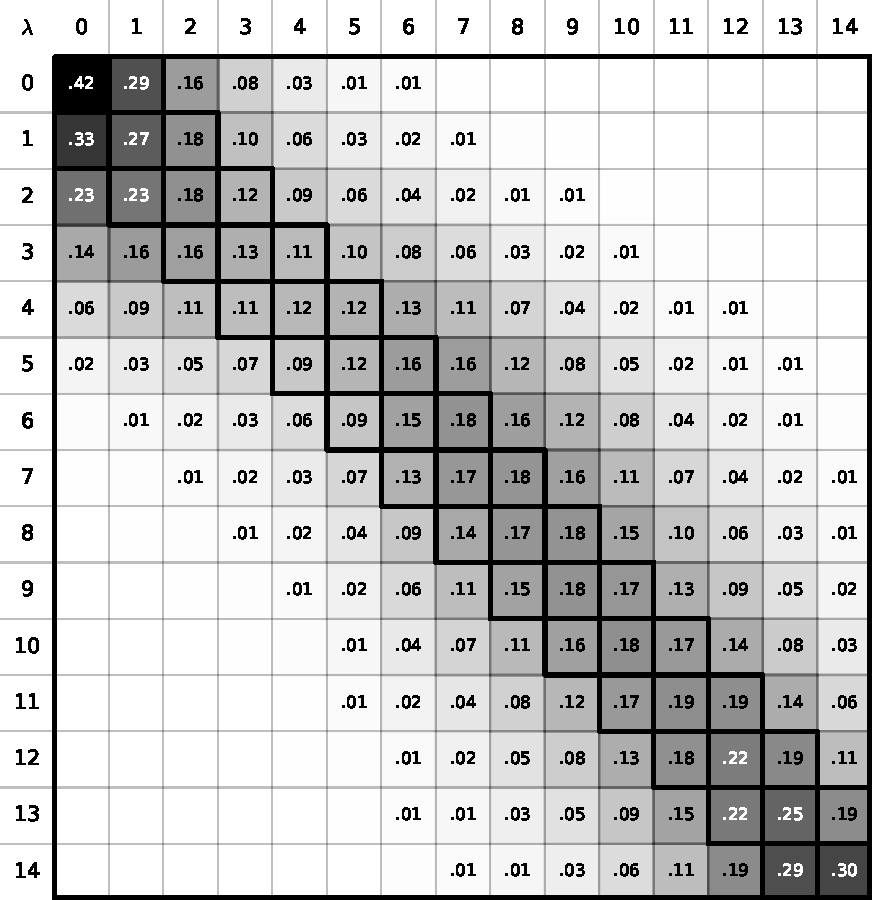
\includegraphics[width=0.9\textwidth]{Figures/ohex_benz}
	\caption{Overlapping matrix for hexane+benzene.}
\end{figure}

\begin{figure}[H]
	\centering
	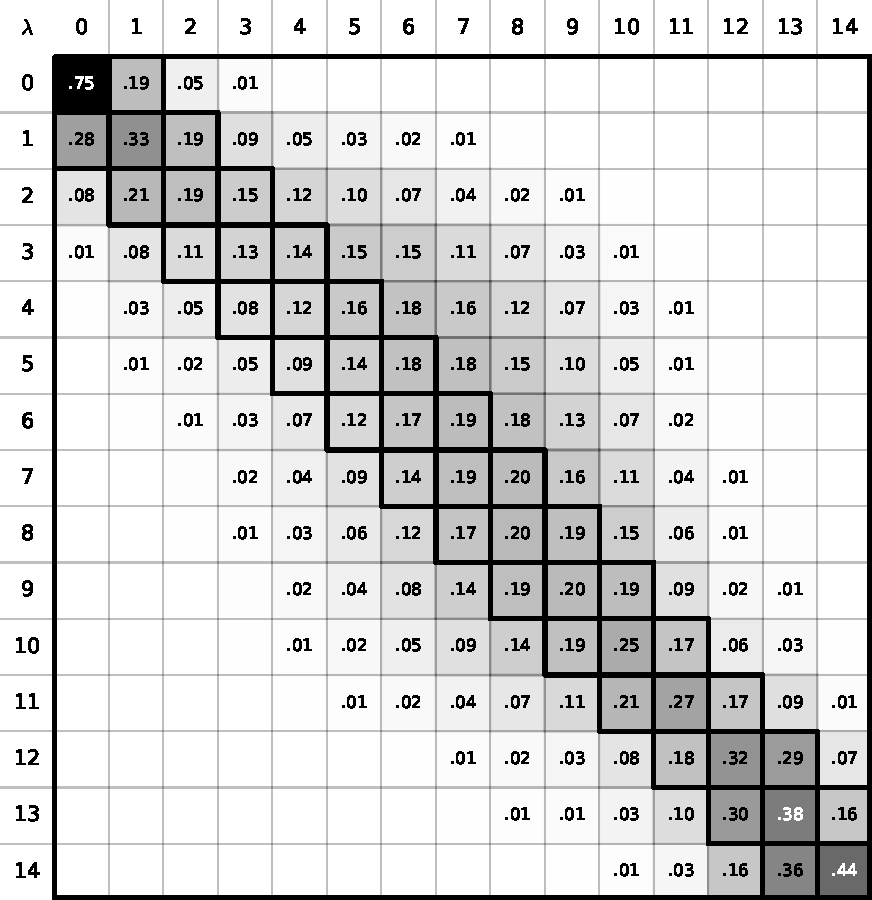
\includegraphics[width=0.9\textwidth]{Figures/ohex_pyr}
	\caption{Overlapping matrix for hexane+pyrene.}
\end{figure}

\begin{figure}[H]
	\centering
	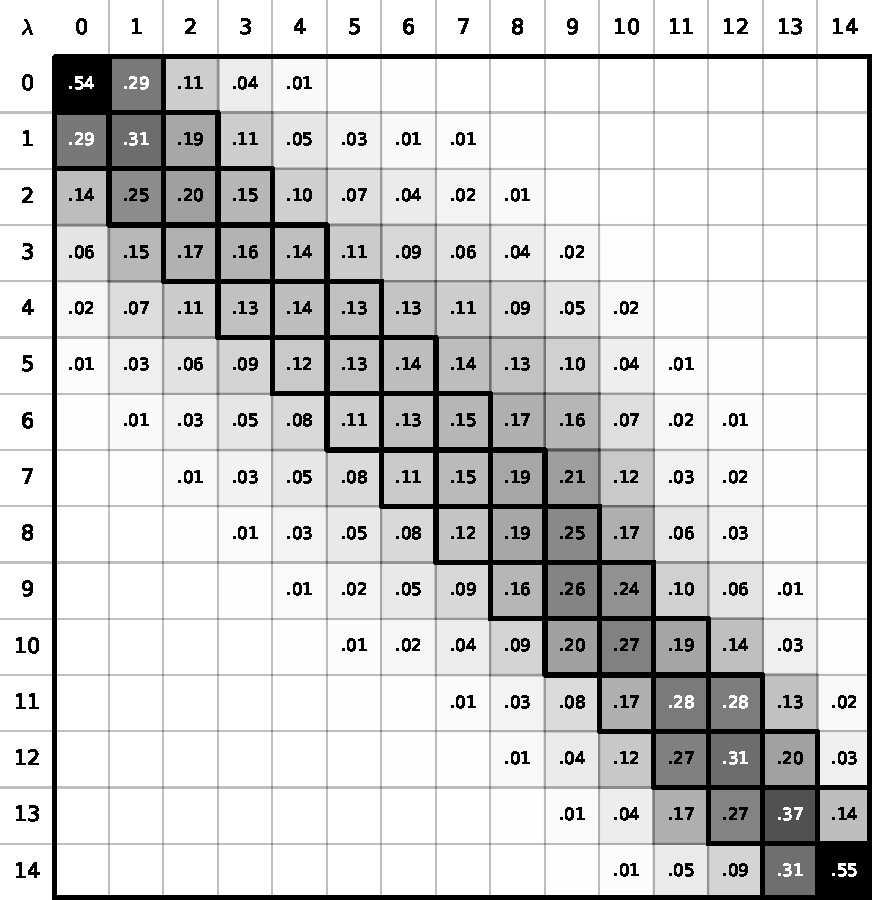
\includegraphics[width=0.9\textwidth]{Figures/ohex_phen}
	\caption{Overlapping matrix for hexane+phenanthrene.}
\end{figure}

\begin{figure}[H]
	\centering
	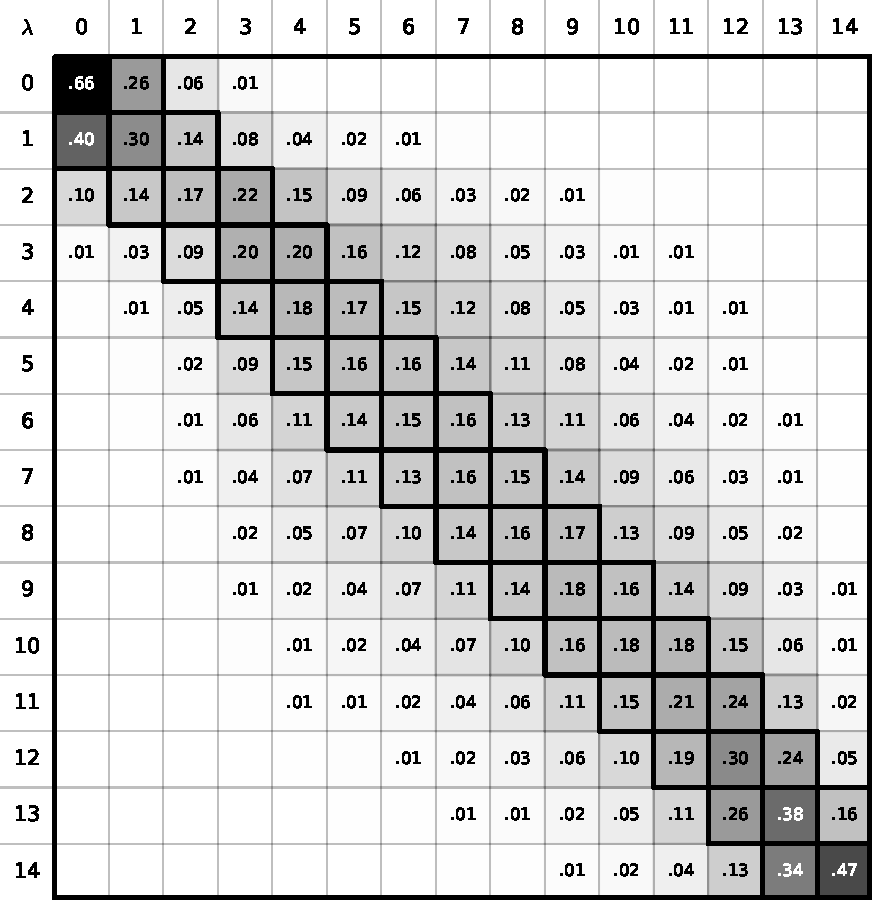
\includegraphics[width=0.9\textwidth]{Figures/ooct_prop}
	\caption{Overlapping matrix for 1-octanol+propane.}
\end{figure}

\begin{figure}[H]
	\centering
	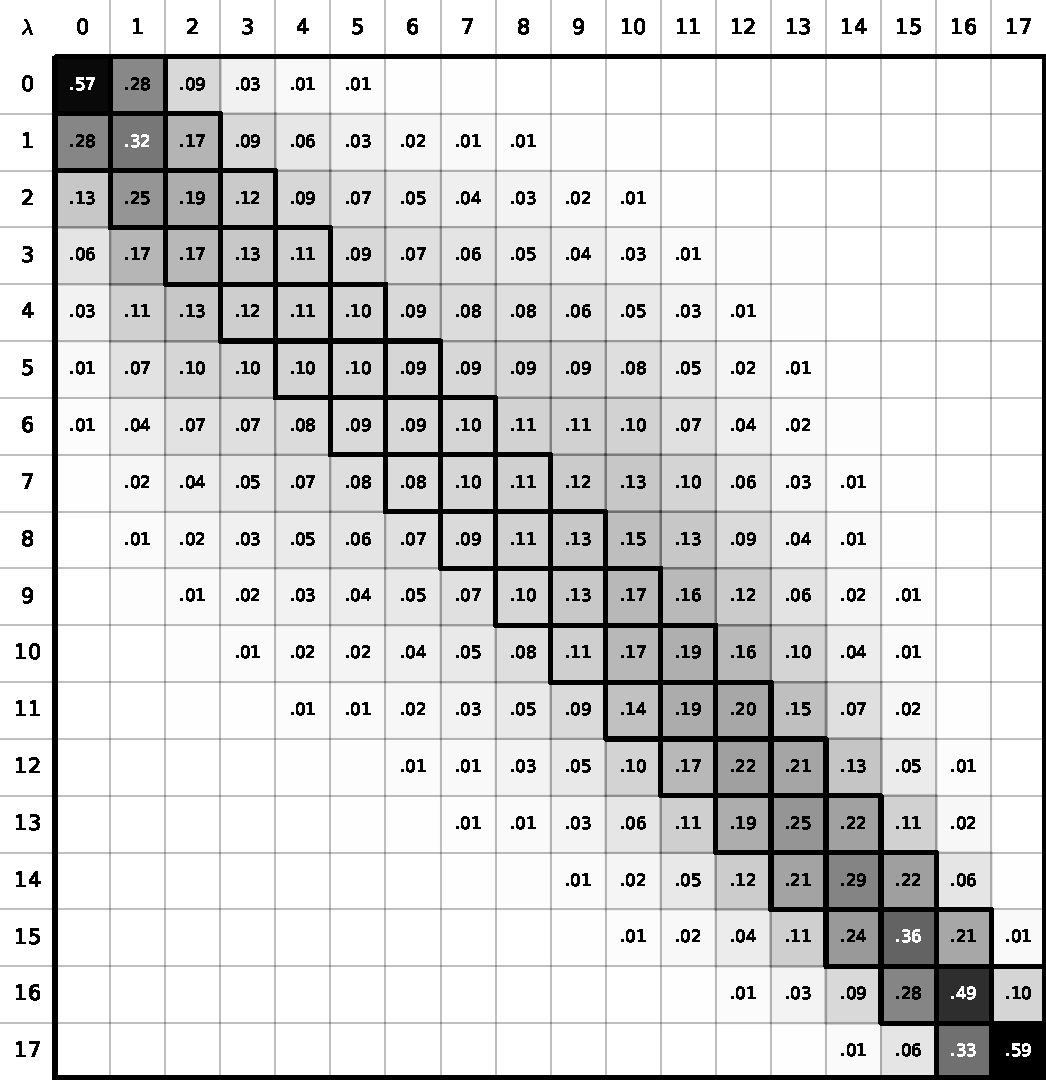
\includegraphics[width=0.9\textwidth]{Figures/ooct_ant}
	\caption{Overlapping matrix for 1-octanol+anthracene.}
\end{figure}

\begin{figure}[H]
	\centering
	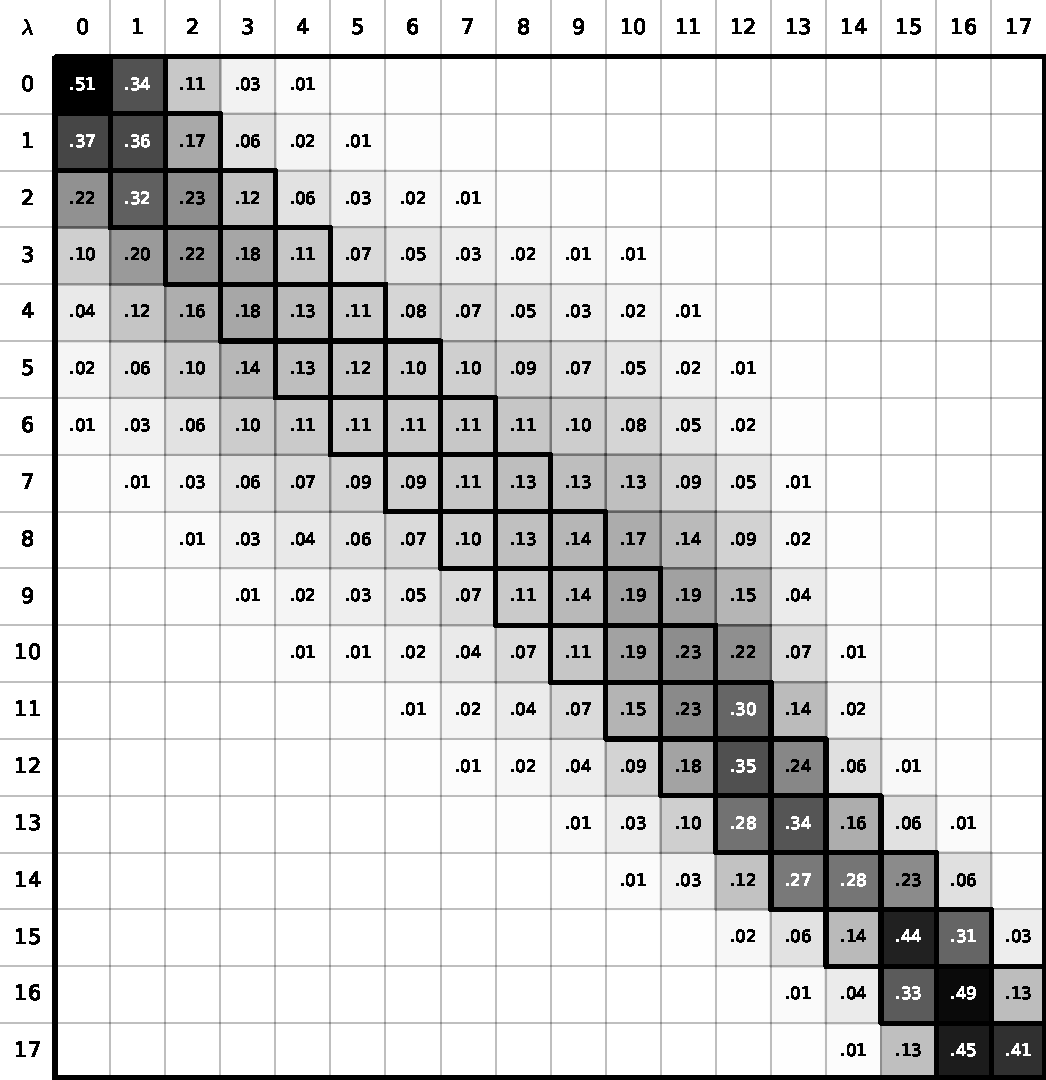
\includegraphics[width=0.9\textwidth]{Figures/ooct_phen}
	\caption{Overlapping matrix for 1-octanol+phenanthrene.}
\end{figure}

\begin{figure}[H]
	\centering
	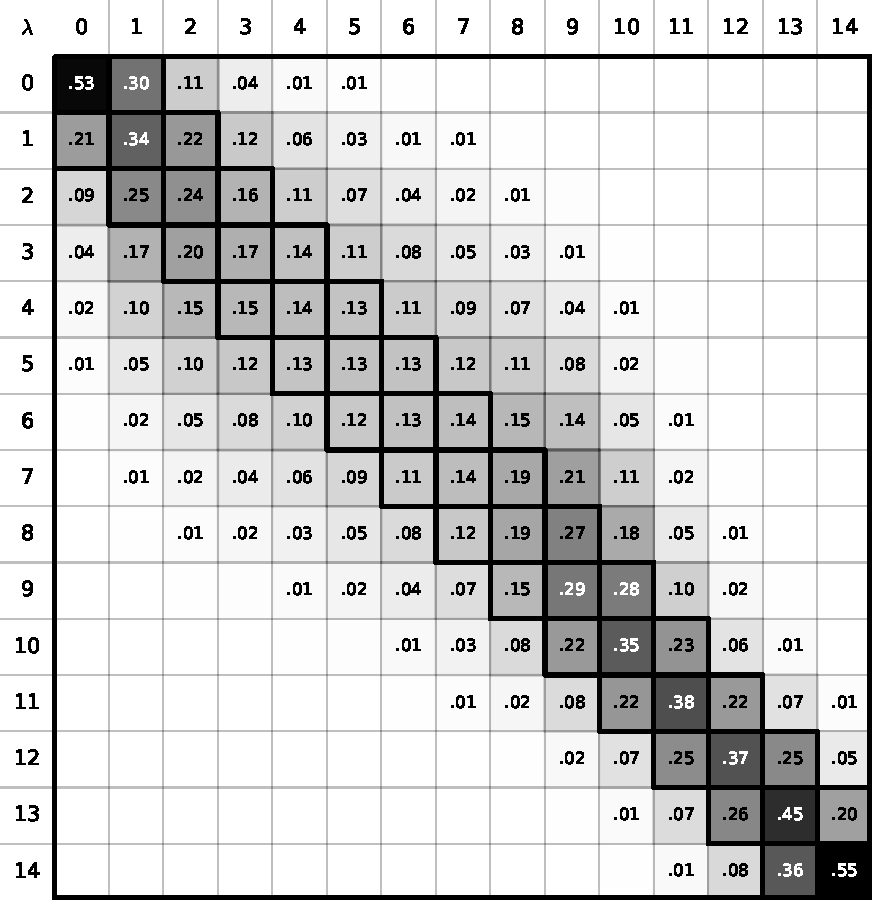
\includegraphics[width=0.9\textwidth]{Figures/otol_pyr}
	\caption{Overlapping matrix for toluene+pyrene.}
\end{figure}

\begin{figure}[H]
	\centering
	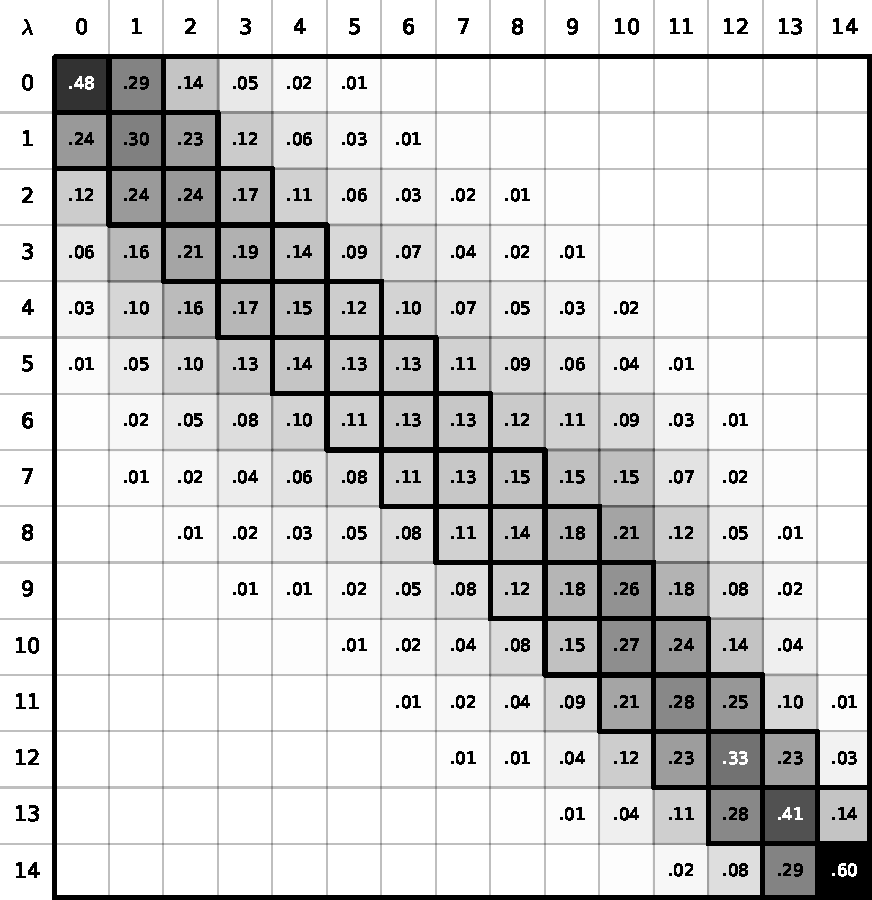
\includegraphics[width=0.9\textwidth]{Figures/otol_antr}
	\caption{Overlapping matrix for toluene+anthracene.}
\end{figure}

\begin{figure}[H]
	\centering
	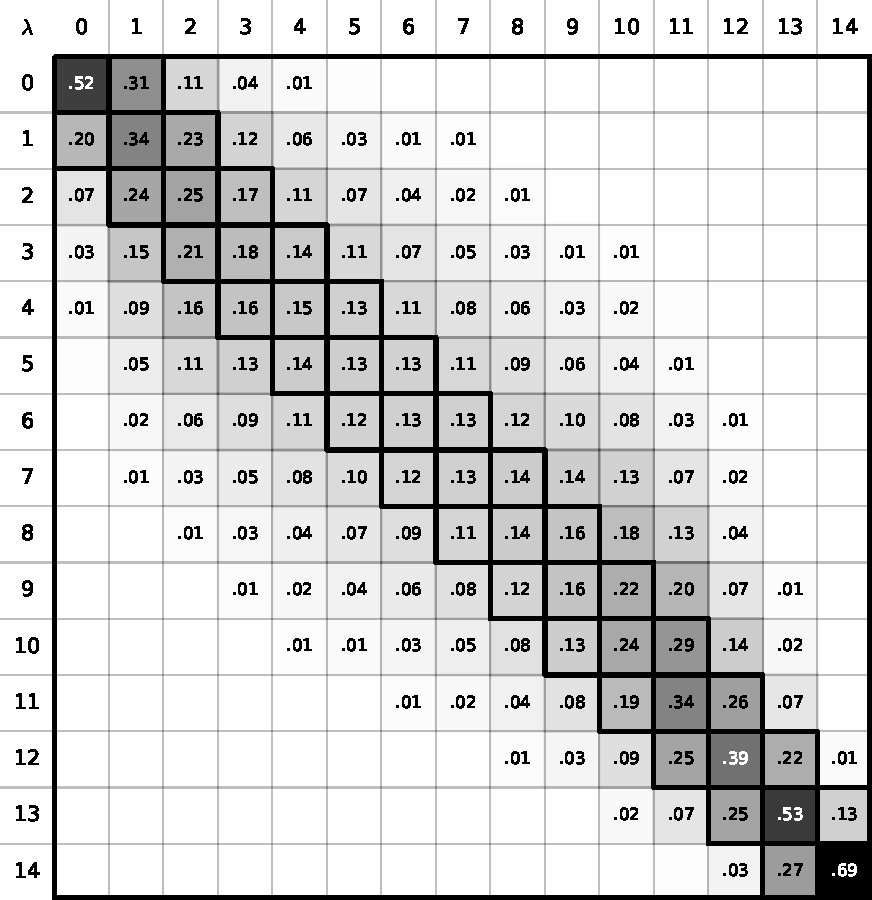
\includegraphics[width=0.9\textwidth]{Figures/otol_phen}
	\caption{Overlapping matrix for toluene+phenanthrene.}
\end{figure}

\begin{figure}[H]
	\centering
	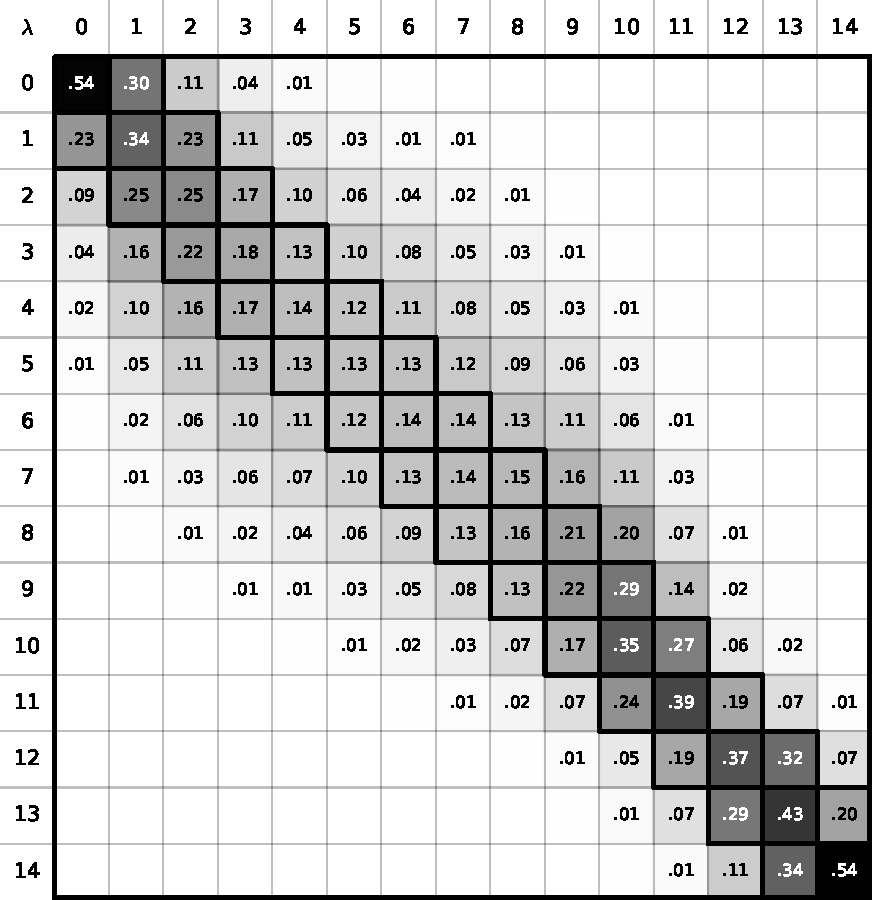
\includegraphics[width=0.9\textwidth]{Figures/otolco2_1}
	\caption{Overlapping matrix for toluene+$CO_{2}$(0.087)+phenanthrene.}
\end{figure}
\begin{figure}[H]
	\centering
	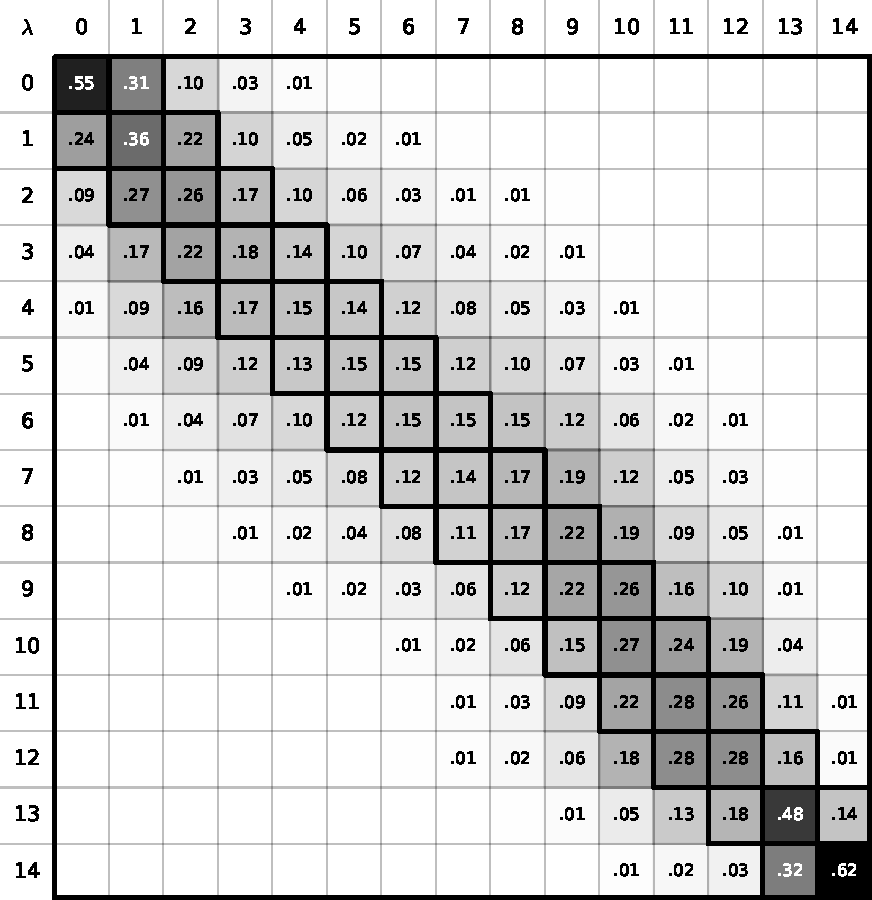
\includegraphics[width=0.9\textwidth]{Figures/otolco2_2}
	\caption{Overlapping matrix for toluene+$CO_{2}$(0.119)+phenanthrene.}
\end{figure}

\begin{figure}[H]
	\centering
	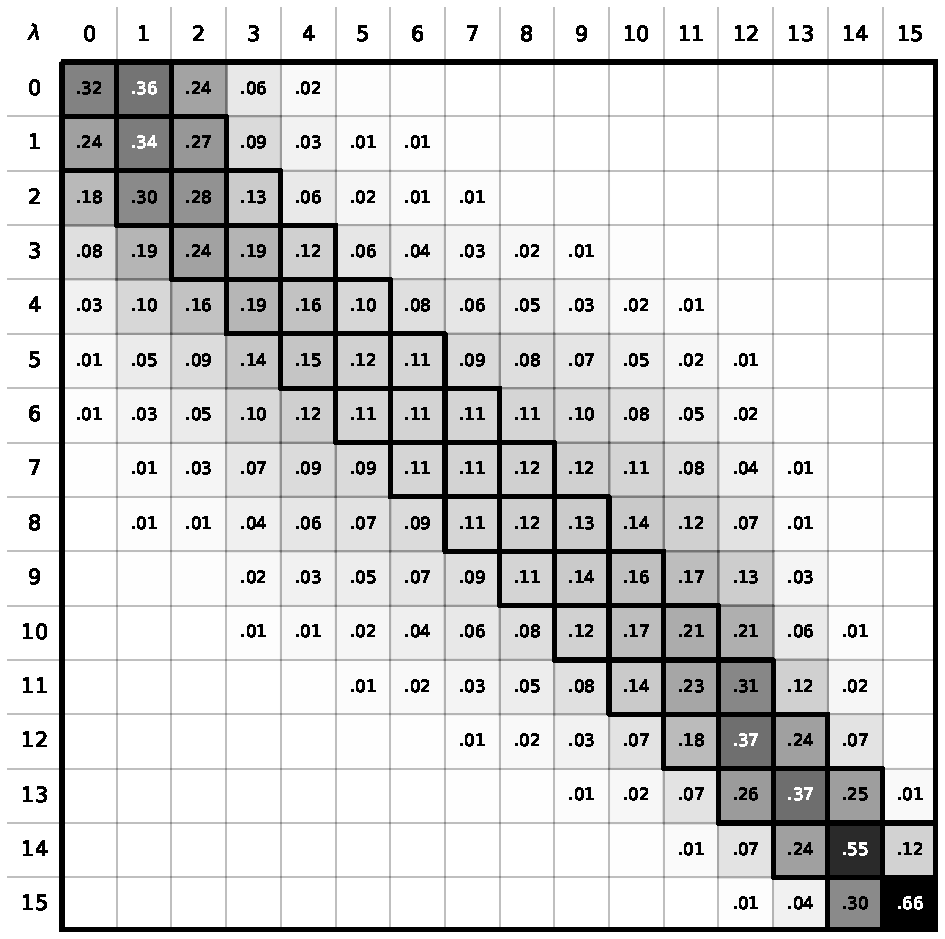
\includegraphics[width=0.9\textwidth]{Figures/otolco2_3}
	\caption{Overlapping matrix for toluene+$CO_{2}$(0.169)+phenanthrene.}
\end{figure}

\begin{figure}[H]
	\centering
	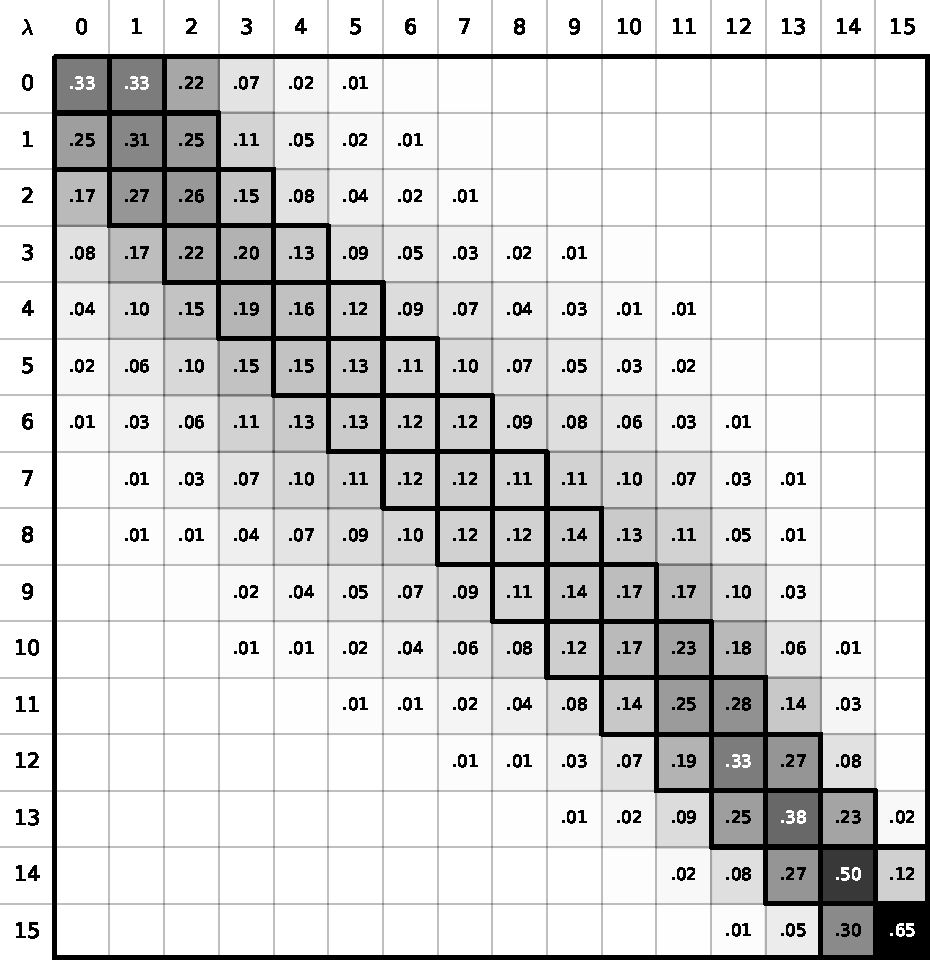
\includegraphics[width=0.9\textwidth]{Figures/otolco2_4}
	\caption{Overlapping matrix for toluene+$CO_{2}$(0.289)+phenanthrene.}
\end{figure}

\begin{figure}[H]
	\centering
	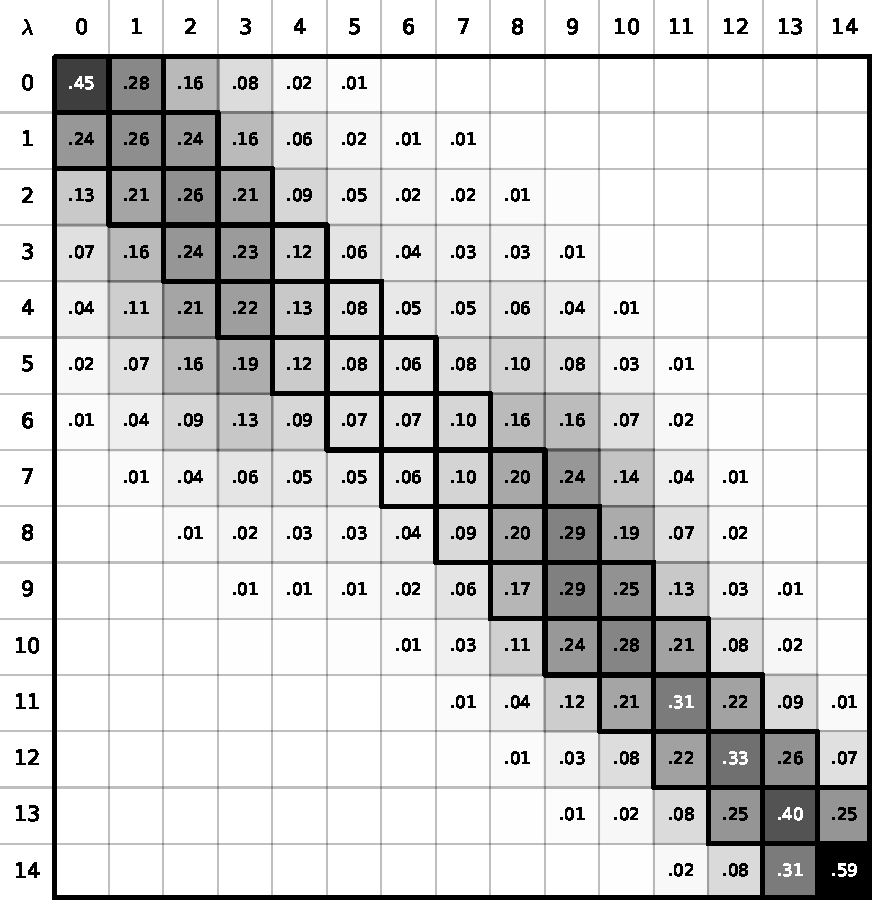
\includegraphics[width=0.9\textwidth]{Figures/owat_prop}
	\caption{Overlapping matrix for water+propane.}
\end{figure}

\begin{figure}[H]
	\centering
	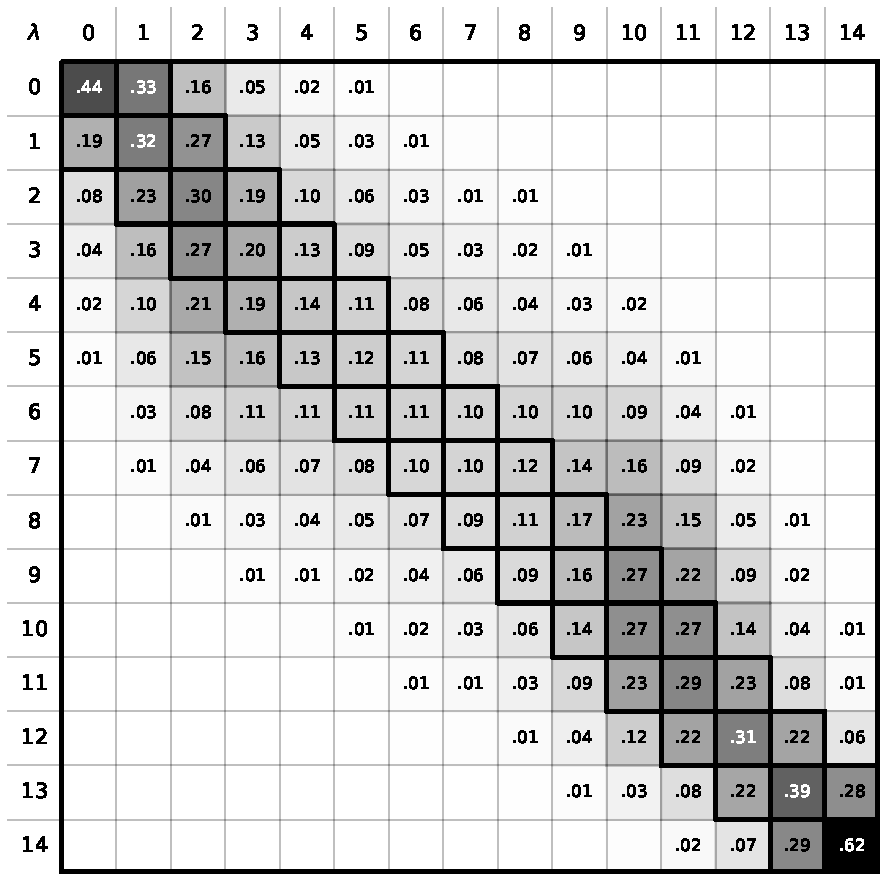
\includegraphics[width=0.9\textwidth]{Figures/owat_benz}
	\caption{Overlapping matrix for water+benzene.}
\end{figure}

\begin{figure}[H]
	\centering
	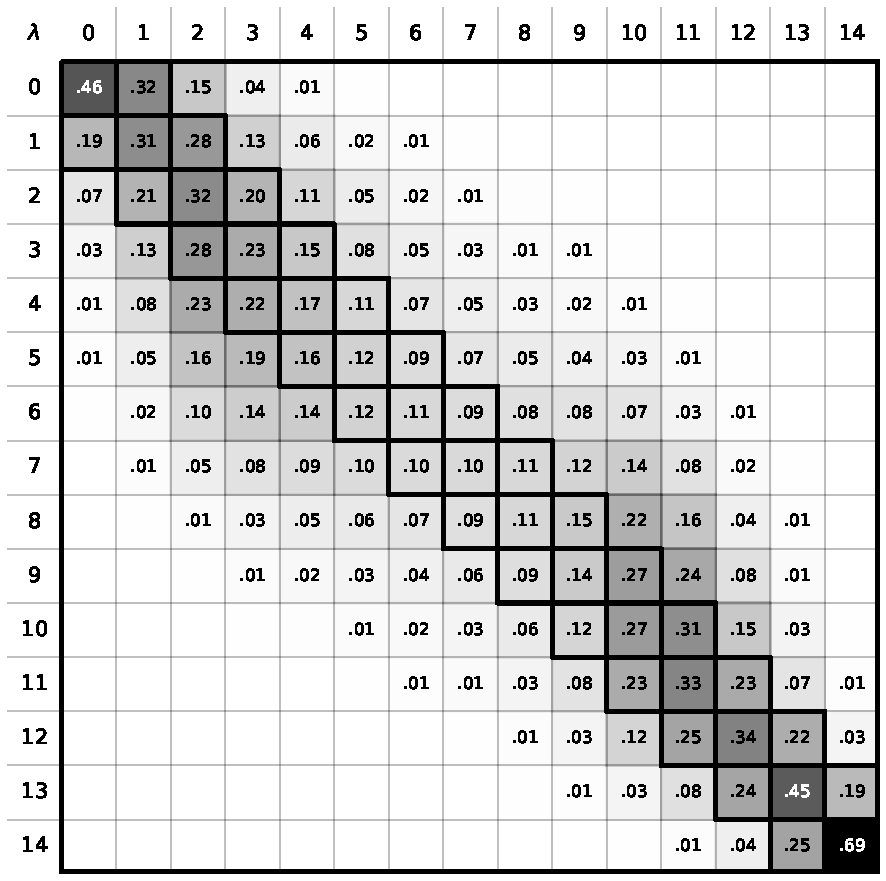
\includegraphics[width=0.9\textwidth]{Figures/owat_tol}
	\caption{Overlapping matrix for water+toluene.}
\end{figure}

\begin{figure}[H]
	\centering
	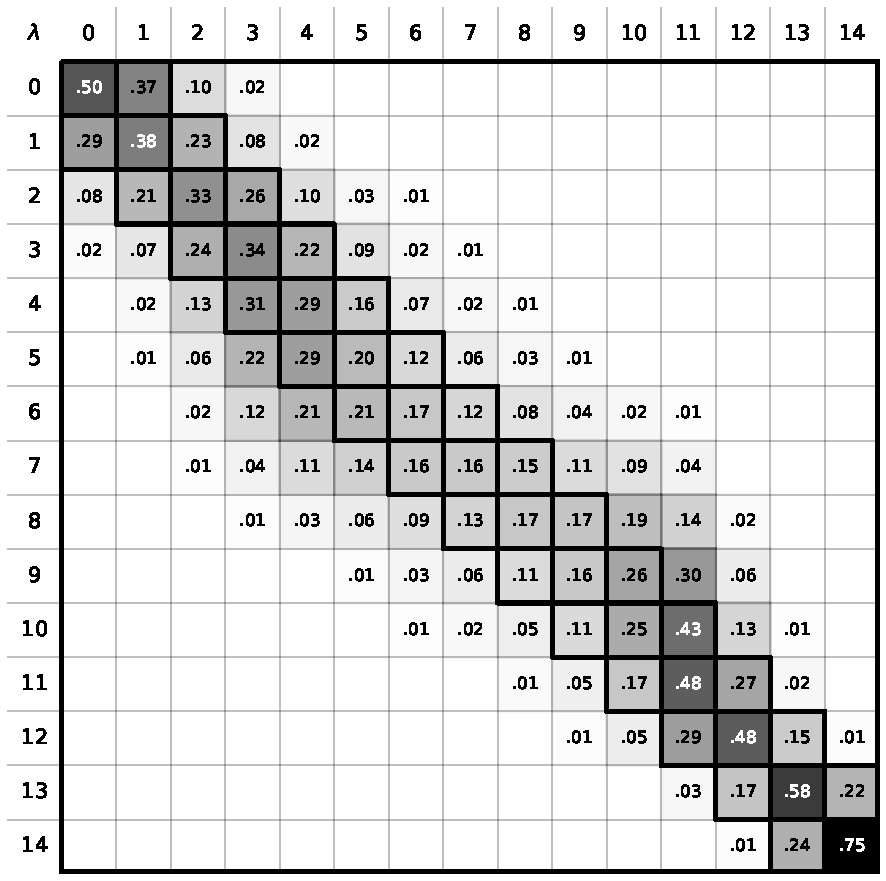
\includegraphics[width=0.9\textwidth]{Figures/owat_phen}
	\caption{Overlapping matrix for water+phenanthrene.}
\end{figure}

\end{apendicesenv}
% ---


% ----------------------------------------------------------
% Anexos
% ----------------------------------------------------------

% ---
% Inicia os anexos
%% ---
%\begin{anexosenv}
%
%% Imprime uma página indicando o início dos anexos
%\partanexos
%
%% ---
%\chapter{Morbi ultrices rutrum lorem.}
%% ---
%
%% ---
%\chapter{Fusce facilisis lacinia dui}
%% ---
%
%\end{anexosenv}

%---------------------------------------------------------------------
% INDICE REMISSIVO
%---------------------------------------------------------------------
\phantompart
\printindex
%---------------------------------------------------------------------

\end{document}
